% LexAgent - IEEE conference paper.
% Build:  paper/build.ps1   (regenerates generated/results.tex from the saved result files, then compiles)
% Every reported number is a macro from generated/results.tex; none is typed by hand.
\documentclass[conference]{IEEEtran}
\IEEEoverridecommandlockouts

\usepackage{cite}
\usepackage{amsmath}
% Tectonic compiles with XeTeX: Times-compatible text and math fonts are loaded by file name.
\usepackage{fontspec}
\usepackage{unicode-math}
\setmainfont{texgyretermes}[Extension=.otf, UprightFont=*-regular, BoldFont=*-bold, ItalicFont=*-italic, BoldItalicFont=*-bolditalic, Ligatures=TeX]
\setsansfont{texgyreheros}[Extension=.otf, UprightFont=*-regular, BoldFont=*-bold, ItalicFont=*-italic, BoldItalicFont=*-bolditalic, Scale=0.92]
\setmonofont{texgyrecursor}[Extension=.otf, UprightFont=*-regular, BoldFont=*-bold, ItalicFont=*-italic, BoldItalicFont=*-bolditalic, Scale=0.92]
\setmathfont{texgyretermes-math.otf}
\usepackage{graphicx}
\usepackage{xcolor}
\usepackage{booktabs}
\usepackage{array}
\usepackage{multirow}
\usepackage{tikz}
\usepackage{pgfplots}
\usepackage{pgfplotstable}
\usepackage{balance}
\usepackage[hidelinks]{hyperref}
\usetikzlibrary{arrows.meta,positioning,shapes.geometric,shapes.misc,calc,fit,backgrounds}
\usepgfplotslibrary{groupplots}
\pgfplotsset{compat=1.17}

% Colour system shared by every figure.
\definecolor{cData}{HTML}{0F9D94}    % sources
\definecolor{cPipe}{HTML}{0B7285}    % pipeline stages
\definecolor{cStore}{HTML}{3B5BDB}   % indexes
\definecolor{cRetr}{HTML}{2A78D6}    % retrieval / LexAgent series
\definecolor{cAgent}{HTML}{7048E8}   % debate lane
\definecolor{cPros}{HTML}{EB6834}    % prosecutor / baseline series
\definecolor{cDef}{HTML}{D6336C}     % defense
\definecolor{cJudge}{HTML}{5B4BC4}   % judge
\definecolor{cVerify}{HTML}{1E9E55}  % citation checker
\definecolor{cCtrl}{HTML}{E0A100}    % controller
\definecolor{cRefl}{HTML}{1098AD}    % reflection
\definecolor{cMemory}{HTML}{9C36B5}  % memory
\definecolor{cUser}{HTML}{495057}    % input / output
\definecolor{cFab}{HTML}{D7263D}     % fabricated
\definecolor{cNeutral}{HTML}{868E96} % unverifiable / neutral

% Generated by paper/make_results.py from the saved result files. Do not edit by hand.
\newcommand{\ResAblAFourASS}{0.913}
\newcommand{\ResAblAFourConf}{0.39}
\newcommand{\ResAblAFourCrashed}{0}
\newcommand{\ResAblAFourHR}{1.22}
\newcommand{\ResAblAFourMinutes}{51}
\newcommand{\ResAblAFourN}{96}
\newcommand{\ResAblAOneASS}{0.909}
\newcommand{\ResAblAOneConf}{0.43}
\newcommand{\ResAblAOneCrashed}{0}
\newcommand{\ResAblAOneHR}{0.00}
\newcommand{\ResAblAOneMinutes}{43}
\newcommand{\ResAblAOneN}{96}
\newcommand{\ResAblASSMax}{0.921}
\newcommand{\ResAblASSMin}{0.909}
\newcommand{\ResAblAThreeASS}{0.921}
\newcommand{\ResAblAThreeConf}{0.57}
\newcommand{\ResAblAThreeCrashed}{0}
\newcommand{\ResAblAThreeHR}{0.00}
\newcommand{\ResAblAThreeMinutes}{177}
\newcommand{\ResAblAThreeN}{96}
\newcommand{\ResAblATwoASS}{0.912}
\newcommand{\ResAblATwoConf}{0.48}
\newcommand{\ResAblATwoCrashed}{0}
\newcommand{\ResAblATwoHR}{0.17}
\newcommand{\ResAblATwoMinutes}{105}
\newcommand{\ResAblATwoN}{96}
\newcommand{\ResAblFullASS}{0.914}
\newcommand{\ResAblFullConf}{0.39}
\newcommand{\ResAblFullCrashed}{0}
\newcommand{\ResAblFullHR}{0.26}
\newcommand{\ResAblFullMinutes}{120}
\newcommand{\ResAblFullN}{96}
\newcommand{\ResAblHRMax}{1.22}
\newcommand{\ResAblHRMin}{0.00}
\newcommand{\ResAblationCases}{96}
\newcommand{\ResAblationComplete}{1}
\newcommand{\ResAudAPIdentity}{1}
\newcommand{\ResAudAThreeDebates}{96}
\newcommand{\ResAudAThreeSupportLost}{28}
\newcommand{\ResAudAThreeSupportedAny}{94}
\newcommand{\ResAudCacheAblAFour}{29}
\newcommand{\ResAudCacheAblAOne}{34}
\newcommand{\ResAudCacheAblAThree}{0}
\newcommand{\ResAudCacheAblATwo}{37}
\newcommand{\ResAudCacheAblFull}{30}
\newcommand{\ResAudCacheAblFullReproduced}{30}
\newcommand{\ResAudCacheAblMax}{37}
\newcommand{\ResAudCacheAblMin}{29}
\newcommand{\ResAudCacheBench}{34}
\newcommand{\ResAudCacheSameTarget}{0}
\newcommand{\ResAudCacheSignatureComplete}{1}
\newcommand{\ResAudCollisionPairs}{151}
\newcommand{\ResAudCollisionPairsTotal}{4{,}560}
\newcommand{\ResAudCollisionQuestions}{48}
\newcommand{\ResAudDebated}{62}
\newcommand{\ResAudDebatedARHigh}{+41.9}
\newcommand{\ResAudDebatedARLow}{+17.7}
\newcommand{\ResAudDebatedARP}{$p<0.001$}
\newcommand{\ResAudDebatedAtMaxRounds}{62}
\newcommand{\ResAudDebatedBaseAR}{51.6}
\newcommand{\ResAudDebatedBelowMaxRounds}{0}
\newcommand{\ResAudDebatedConf}{0.57}
\newcommand{\ResAudDebatedLexAR}{80.6}
\newcommand{\ResAudImpliedConfAThree}{0.57}
\newcommand{\ResAudImpliedConfFull}{0.56}
\newcommand{\ResAudNoCollisionThreshold}{0.9625}
\newcommand{\ResAudSimFloor}{0.876}
\newcommand{\ResAudSimQuestion}{0.931}
\newcommand{\ResBaseAP}{47.2}
\newcommand{\ResBaseAR}{59.4}
\newcommand{\ResBaseASS}{0.940}
\newcommand{\ResBaseASSpct}{94.0}
\newcommand{\ResBaseCites}{118}
\newcommand{\ResBaseCitesPerAnswer}{1.23}
\newcommand{\ResBaseFlagged}{3}
\newcommand{\ResBaseFlaggedCases}{2}
\newcommand{\ResBaseHR}{2.08}
\newcommand{\ResBaseNoCiteAnswers}{13}
\newcommand{\ResBaseNoCitePct}{13.5}
\newcommand{\ResCmpBaseEightBaseFourCitesAllDiff}{+0.39}
\newcommand{\ResCmpBaseEightBaseFourCitesAllHigh}{+0.59}
\newcommand{\ResCmpBaseEightBaseFourCitesAllLow}{+0.20}
\newcommand{\ResCmpBaseEightBaseFourCitesAllMark}{$^{\ast}$}
\newcommand{\ResCmpBaseEightBaseFourCitesAllP}{$p<0.001$}
\newcommand{\ResCmpBaseEightBaseFourCitesAllWord}{significant}
\newcommand{\ResCmpBaseEightBaseFourCitesAnswerDiff}{+0.39}
\newcommand{\ResCmpBaseEightBaseFourCitesAnswerHigh}{+0.59}
\newcommand{\ResCmpBaseEightBaseFourCitesAnswerLow}{+0.20}
\newcommand{\ResCmpBaseEightBaseFourCitesAnswerMark}{$^{\ast}$}
\newcommand{\ResCmpBaseEightBaseFourCitesAnswerP}{$p<0.001$}
\newcommand{\ResCmpBaseEightBaseFourCitesAnswerWord}{significant}
\newcommand{\ResCmpBaseEightBaseFourNoAuthorityDiff}{+1.7}
\newcommand{\ResCmpBaseEightBaseFourNoAuthorityHigh}{+5.2}
\newcommand{\ResCmpBaseEightBaseFourNoAuthorityLow}{$-$1.4}
\newcommand{\ResCmpBaseEightBaseFourNoAuthorityMark}{}
\newcommand{\ResCmpBaseEightBaseFourNoAuthorityP}{$p=0.438$}
\newcommand{\ResCmpBaseEightBaseFourNoAuthorityWord}{not significant}
\newcommand{\ResCmpBaseEightBaseFourSimDiff}{+0.013}
\newcommand{\ResCmpBaseEightBaseFourSimHigh}{+0.022}
\newcommand{\ResCmpBaseEightBaseFourSimLow}{+0.005}
\newcommand{\ResCmpBaseEightBaseFourSimMark}{$^{\ast}$}
\newcommand{\ResCmpBaseEightBaseFourSimP}{$p=0.003$}
\newcommand{\ResCmpBaseEightBaseFourSimWord}{significant}
\newcommand{\ResCmpBaseEightBaseFourTargetAnswerDiff}{+6.2}
\newcommand{\ResCmpBaseEightBaseFourTargetAnswerHigh}{+13.5}
\newcommand{\ResCmpBaseEightBaseFourTargetAnswerLow}{$-$1.4}
\newcommand{\ResCmpBaseEightBaseFourTargetAnswerMark}{}
\newcommand{\ResCmpBaseEightBaseFourTargetAnswerP}{$p=0.133$}
\newcommand{\ResCmpBaseEightBaseFourTargetAnswerWord}{not significant}
\newcommand{\ResCmpBaseEightBaseFourTargetAnyDiff}{+6.2}
\newcommand{\ResCmpBaseEightBaseFourTargetAnyHigh}{+13.5}
\newcommand{\ResCmpBaseEightBaseFourTargetAnyLow}{$-$1.4}
\newcommand{\ResCmpBaseEightBaseFourTargetAnyMark}{}
\newcommand{\ResCmpBaseEightBaseFourTargetAnyP}{$p=0.133$}
\newcommand{\ResCmpBaseEightBaseFourTargetAnyWord}{not significant}
\newcommand{\ResCmpBaseEightRBaseEightCitesAllDiff}{+0.7}
\newcommand{\ResCmpBaseEightRBaseEightCitesAllHigh}{+1.0}
\newcommand{\ResCmpBaseEightRBaseEightCitesAllLow}{+0.4}
\newcommand{\ResCmpBaseEightRBaseEightCitesAllMark}{$^{\ast}$}
\newcommand{\ResCmpBaseEightRBaseEightCitesAllP}{$p<0.001$}
\newcommand{\ResCmpBaseEightRBaseEightCitesAllWord}{significant}
\newcommand{\ResCmpBaseEightRBaseEightCitesAnswerDiff}{+0.7}
\newcommand{\ResCmpBaseEightRBaseEightCitesAnswerHigh}{+1.0}
\newcommand{\ResCmpBaseEightRBaseEightCitesAnswerLow}{+0.4}
\newcommand{\ResCmpBaseEightRBaseEightCitesAnswerMark}{$^{\ast}$}
\newcommand{\ResCmpBaseEightRBaseEightCitesAnswerP}{$p<0.001$}
\newcommand{\ResCmpBaseEightRBaseEightCitesAnswerWord}{significant}
\newcommand{\ResCmpBaseEightRBaseEightNoAuthorityDiff}{+6.6}
\newcommand{\ResCmpBaseEightRBaseEightNoAuthorityHigh}{+12.8}
\newcommand{\ResCmpBaseEightRBaseEightNoAuthorityLow}{+0.4}
\newcommand{\ResCmpBaseEightRBaseEightNoAuthorityMark}{}
\newcommand{\ResCmpBaseEightRBaseEightNoAuthorityP}{$p=0.050$}
\newcommand{\ResCmpBaseEightRBaseEightNoAuthorityWord}{not significant}
\newcommand{\ResCmpBaseEightRBaseEightSimDiff}{+0.004}
\newcommand{\ResCmpBaseEightRBaseEightSimHigh}{+0.014}
\newcommand{\ResCmpBaseEightRBaseEightSimLow}{$-$0.006}
\newcommand{\ResCmpBaseEightRBaseEightSimMark}{}
\newcommand{\ResCmpBaseEightRBaseEightSimP}{$p=0.424$}
\newcommand{\ResCmpBaseEightRBaseEightSimWord}{not significant}
\newcommand{\ResCmpBaseEightRBaseEightTargetAnswerDiff}{+3.1}
\newcommand{\ResCmpBaseEightRBaseEightTargetAnswerHigh}{+11.8}
\newcommand{\ResCmpBaseEightRBaseEightTargetAnswerLow}{$-$5.2}
\newcommand{\ResCmpBaseEightRBaseEightTargetAnswerMark}{}
\newcommand{\ResCmpBaseEightRBaseEightTargetAnswerP}{$p=0.528$}
\newcommand{\ResCmpBaseEightRBaseEightTargetAnswerWord}{not significant}
\newcommand{\ResCmpBaseEightRBaseEightTargetAnyDiff}{+3.1}
\newcommand{\ResCmpBaseEightRBaseEightTargetAnyHigh}{+11.8}
\newcommand{\ResCmpBaseEightRBaseEightTargetAnyLow}{$-$5.2}
\newcommand{\ResCmpBaseEightRBaseEightTargetAnyMark}{}
\newcommand{\ResCmpBaseEightRBaseEightTargetAnyP}{$p=0.528$}
\newcommand{\ResCmpBaseEightRBaseEightTargetAnyWord}{not significant}
\newcommand{\ResCmpBaseEightRBaseFourRCitesAllDiff}{+0.7}
\newcommand{\ResCmpBaseEightRBaseFourRCitesAllHigh}{+1.0}
\newcommand{\ResCmpBaseEightRBaseFourRCitesAllLow}{+0.5}
\newcommand{\ResCmpBaseEightRBaseFourRCitesAllMark}{$^{\ast}$}
\newcommand{\ResCmpBaseEightRBaseFourRCitesAllP}{$p<0.001$}
\newcommand{\ResCmpBaseEightRBaseFourRCitesAllWord}{significant}
\newcommand{\ResCmpBaseEightRBaseFourRCitesAnswerDiff}{+0.7}
\newcommand{\ResCmpBaseEightRBaseFourRCitesAnswerHigh}{+1.0}
\newcommand{\ResCmpBaseEightRBaseFourRCitesAnswerLow}{+0.5}
\newcommand{\ResCmpBaseEightRBaseFourRCitesAnswerMark}{$^{\ast}$}
\newcommand{\ResCmpBaseEightRBaseFourRCitesAnswerP}{$p<0.001$}
\newcommand{\ResCmpBaseEightRBaseFourRCitesAnswerWord}{significant}
\newcommand{\ResCmpBaseEightRBaseFourRNoAuthorityDiff}{+9.0}
\newcommand{\ResCmpBaseEightRBaseFourRNoAuthorityHigh}{+14.9}
\newcommand{\ResCmpBaseEightRBaseFourRNoAuthorityLow}{+3.5}
\newcommand{\ResCmpBaseEightRBaseFourRNoAuthorityMark}{$^{\ast}$}
\newcommand{\ResCmpBaseEightRBaseFourRNoAuthorityP}{$p=0.003$}
\newcommand{\ResCmpBaseEightRBaseFourRNoAuthorityWord}{significant}
\newcommand{\ResCmpBaseEightRBaseFourRSimDiff}{+0.003}
\newcommand{\ResCmpBaseEightRBaseFourRSimHigh}{+0.011}
\newcommand{\ResCmpBaseEightRBaseFourRSimLow}{$-$0.005}
\newcommand{\ResCmpBaseEightRBaseFourRSimMark}{}
\newcommand{\ResCmpBaseEightRBaseFourRSimP}{$p=0.480$}
\newcommand{\ResCmpBaseEightRBaseFourRSimWord}{not significant}
\newcommand{\ResCmpBaseEightRBaseFourRTargetAnswerDiff}{$-$4.5}
\newcommand{\ResCmpBaseEightRBaseFourRTargetAnswerHigh}{+3.5}
\newcommand{\ResCmpBaseEightRBaseFourRTargetAnswerLow}{$-$13.2}
\newcommand{\ResCmpBaseEightRBaseFourRTargetAnswerMark}{}
\newcommand{\ResCmpBaseEightRBaseFourRTargetAnswerP}{$p=0.331$}
\newcommand{\ResCmpBaseEightRBaseFourRTargetAnswerWord}{not significant}
\newcommand{\ResCmpBaseEightRBaseFourRTargetAnyDiff}{$-$4.5}
\newcommand{\ResCmpBaseEightRBaseFourRTargetAnyHigh}{+3.5}
\newcommand{\ResCmpBaseEightRBaseFourRTargetAnyLow}{$-$13.2}
\newcommand{\ResCmpBaseEightRBaseFourRTargetAnyMark}{}
\newcommand{\ResCmpBaseEightRBaseFourRTargetAnyP}{$p=0.331$}
\newcommand{\ResCmpBaseEightRBaseFourRTargetAnyWord}{not significant}
\newcommand{\ResCmpBaseFourRBaseFourCitesAllDiff}{+0.4}
\newcommand{\ResCmpBaseFourRBaseFourCitesAllHigh}{+0.6}
\newcommand{\ResCmpBaseFourRBaseFourCitesAllLow}{+0.2}
\newcommand{\ResCmpBaseFourRBaseFourCitesAllMark}{$^{\ast}$}
\newcommand{\ResCmpBaseFourRBaseFourCitesAllP}{$p<0.001$}
\newcommand{\ResCmpBaseFourRBaseFourCitesAllWord}{significant}
\newcommand{\ResCmpBaseFourRBaseFourCitesAnswerDiff}{+0.4}
\newcommand{\ResCmpBaseFourRBaseFourCitesAnswerHigh}{+0.6}
\newcommand{\ResCmpBaseFourRBaseFourCitesAnswerLow}{+0.2}
\newcommand{\ResCmpBaseFourRBaseFourCitesAnswerMark}{$^{\ast}$}
\newcommand{\ResCmpBaseFourRBaseFourCitesAnswerP}{$p<0.001$}
\newcommand{\ResCmpBaseFourRBaseFourCitesAnswerWord}{significant}
\newcommand{\ResCmpBaseFourRBaseFourNoAuthorityDiff}{$-$0.7}
\newcommand{\ResCmpBaseFourRBaseFourNoAuthorityHigh}{+2.4}
\newcommand{\ResCmpBaseFourRBaseFourNoAuthorityLow}{$-$3.8}
\newcommand{\ResCmpBaseFourRBaseFourNoAuthorityMark}{}
\newcommand{\ResCmpBaseFourRBaseFourNoAuthorityP}{$p=1.000$}
\newcommand{\ResCmpBaseFourRBaseFourNoAuthorityWord}{not significant}
\newcommand{\ResCmpBaseFourRBaseFourSimDiff}{+0.014}
\newcommand{\ResCmpBaseFourRBaseFourSimHigh}{+0.022}
\newcommand{\ResCmpBaseFourRBaseFourSimLow}{+0.007}
\newcommand{\ResCmpBaseFourRBaseFourSimMark}{$^{\ast}$}
\newcommand{\ResCmpBaseFourRBaseFourSimP}{$p<0.001$}
\newcommand{\ResCmpBaseFourRBaseFourSimWord}{significant}
\newcommand{\ResCmpBaseFourRBaseFourTargetAnswerDiff}{+13.9}
\newcommand{\ResCmpBaseFourRBaseFourTargetAnswerHigh}{+22.6}
\newcommand{\ResCmpBaseFourRBaseFourTargetAnswerLow}{+5.2}
\newcommand{\ResCmpBaseFourRBaseFourTargetAnswerMark}{$^{\ast}$}
\newcommand{\ResCmpBaseFourRBaseFourTargetAnswerP}{$p=0.003$}
\newcommand{\ResCmpBaseFourRBaseFourTargetAnswerWord}{significant}
\newcommand{\ResCmpBaseFourRBaseFourTargetAnyDiff}{+13.9}
\newcommand{\ResCmpBaseFourRBaseFourTargetAnyHigh}{+22.6}
\newcommand{\ResCmpBaseFourRBaseFourTargetAnyLow}{+5.2}
\newcommand{\ResCmpBaseFourRBaseFourTargetAnyMark}{$^{\ast}$}
\newcommand{\ResCmpBaseFourRBaseFourTargetAnyP}{$p=0.003$}
\newcommand{\ResCmpBaseFourRBaseFourTargetAnyWord}{significant}
\newcommand{\ResCmpFinalBaseEightRCitesAllDiff}{+0.2}
\newcommand{\ResCmpFinalBaseEightRCitesAllHigh}{+0.5}
\newcommand{\ResCmpFinalBaseEightRCitesAllLow}{$-$0.1}
\newcommand{\ResCmpFinalBaseEightRCitesAllMark}{}
\newcommand{\ResCmpFinalBaseEightRCitesAllP}{$p=0.157$}
\newcommand{\ResCmpFinalBaseEightRCitesAllWord}{not significant}
\newcommand{\ResCmpFinalBaseEightRCitesAnswerDiff}{$-$1.4}
\newcommand{\ResCmpFinalBaseEightRCitesAnswerHigh}{$-$1.1}
\newcommand{\ResCmpFinalBaseEightRCitesAnswerLow}{$-$1.7}
\newcommand{\ResCmpFinalBaseEightRCitesAnswerMark}{$^{\ast}$}
\newcommand{\ResCmpFinalBaseEightRCitesAnswerP}{$p<0.001$}
\newcommand{\ResCmpFinalBaseEightRCitesAnswerWord}{significant}
\newcommand{\ResCmpFinalBaseEightRNoAuthorityDiff}{+1.4}
\newcommand{\ResCmpFinalBaseEightRNoAuthorityHigh}{+8.0}
\newcommand{\ResCmpFinalBaseEightRNoAuthorityLow}{$-$5.6}
\newcommand{\ResCmpFinalBaseEightRNoAuthorityMark}{}
\newcommand{\ResCmpFinalBaseEightRNoAuthorityP}{$p=0.757$}
\newcommand{\ResCmpFinalBaseEightRNoAuthorityWord}{not significant}
\newcommand{\ResCmpFinalBaseEightRSimDiff}{$-$0.061}
\newcommand{\ResCmpFinalBaseEightRSimHigh}{$-$0.041}
\newcommand{\ResCmpFinalBaseEightRSimLow}{$-$0.082}
\newcommand{\ResCmpFinalBaseEightRSimMark}{$^{\ast}$}
\newcommand{\ResCmpFinalBaseEightRSimP}{$p<0.001$}
\newcommand{\ResCmpFinalBaseEightRSimWord}{significant}
\newcommand{\ResCmpFinalBaseEightRTargetAnswerDiff}{$-$14.6}
\newcommand{\ResCmpFinalBaseEightRTargetAnswerHigh}{$-$5.9}
\newcommand{\ResCmpFinalBaseEightRTargetAnswerLow}{$-$23.3}
\newcommand{\ResCmpFinalBaseEightRTargetAnswerMark}{$^{\ast}$}
\newcommand{\ResCmpFinalBaseEightRTargetAnswerP}{$p=0.002$}
\newcommand{\ResCmpFinalBaseEightRTargetAnswerWord}{significant}
\newcommand{\ResCmpFinalBaseEightRTargetAnyDiff}{+5.9}
\newcommand{\ResCmpFinalBaseEightRTargetAnyHigh}{+14.2}
\newcommand{\ResCmpFinalBaseEightRTargetAnyLow}{$-$2.1}
\newcommand{\ResCmpFinalBaseEightRTargetAnyMark}{}
\newcommand{\ResCmpFinalBaseEightRTargetAnyP}{$p=0.181$}
\newcommand{\ResCmpFinalBaseEightRTargetAnyWord}{not significant}
\newcommand{\ResCmpFinalBaseFourCitesAllDiff}{+1.3}
\newcommand{\ResCmpFinalBaseFourCitesAllHigh}{+1.5}
\newcommand{\ResCmpFinalBaseFourCitesAllLow}{+1.1}
\newcommand{\ResCmpFinalBaseFourCitesAllMark}{$^{\ast}$}
\newcommand{\ResCmpFinalBaseFourCitesAllP}{$p<0.001$}
\newcommand{\ResCmpFinalBaseFourCitesAllWord}{significant}
\newcommand{\ResCmpFinalBaseFourCitesAnswerDiff}{$-$0.3}
\newcommand{\ResCmpFinalBaseFourCitesAnswerHigh}{$-$0.1}
\newcommand{\ResCmpFinalBaseFourCitesAnswerLow}{$-$0.4}
\newcommand{\ResCmpFinalBaseFourCitesAnswerMark}{$^{\ast}$}
\newcommand{\ResCmpFinalBaseFourCitesAnswerP}{$p<0.001$}
\newcommand{\ResCmpFinalBaseFourCitesAnswerWord}{significant}
\newcommand{\ResCmpFinalBaseFourNoAuthorityDiff}{+9.7}
\newcommand{\ResCmpFinalBaseFourNoAuthorityHigh}{+14.6}
\newcommand{\ResCmpFinalBaseFourNoAuthorityLow}{+5.2}
\newcommand{\ResCmpFinalBaseFourNoAuthorityMark}{$^{\ast}$}
\newcommand{\ResCmpFinalBaseFourNoAuthorityP}{$p<0.001$}
\newcommand{\ResCmpFinalBaseFourNoAuthorityWord}{significant}
\newcommand{\ResCmpFinalBaseFourRCitesAllDiff}{+0.9}
\newcommand{\ResCmpFinalBaseFourRCitesAllHigh}{+1.1}
\newcommand{\ResCmpFinalBaseFourRCitesAllLow}{+0.7}
\newcommand{\ResCmpFinalBaseFourRCitesAllMark}{$^{\ast}$}
\newcommand{\ResCmpFinalBaseFourRCitesAllP}{$p<0.001$}
\newcommand{\ResCmpFinalBaseFourRCitesAllWord}{significant}
\newcommand{\ResCmpFinalBaseFourRCitesAnswerDiff}{$-$0.7}
\newcommand{\ResCmpFinalBaseFourRCitesAnswerHigh}{$-$0.5}
\newcommand{\ResCmpFinalBaseFourRCitesAnswerLow}{$-$0.8}
\newcommand{\ResCmpFinalBaseFourRCitesAnswerMark}{$^{\ast}$}
\newcommand{\ResCmpFinalBaseFourRCitesAnswerP}{$p<0.001$}
\newcommand{\ResCmpFinalBaseFourRCitesAnswerWord}{significant}
\newcommand{\ResCmpFinalBaseFourRNoAuthorityDiff}{+10.4}
\newcommand{\ResCmpFinalBaseFourRNoAuthorityHigh}{+14.9}
\newcommand{\ResCmpFinalBaseFourRNoAuthorityLow}{+6.2}
\newcommand{\ResCmpFinalBaseFourRNoAuthorityMark}{$^{\ast}$}
\newcommand{\ResCmpFinalBaseFourRNoAuthorityP}{$p<0.001$}
\newcommand{\ResCmpFinalBaseFourRNoAuthorityWord}{significant}
\newcommand{\ResCmpFinalBaseFourRSimDiff}{$-$0.058}
\newcommand{\ResCmpFinalBaseFourRSimHigh}{$-$0.036}
\newcommand{\ResCmpFinalBaseFourRSimLow}{$-$0.080}
\newcommand{\ResCmpFinalBaseFourRSimMark}{$^{\ast}$}
\newcommand{\ResCmpFinalBaseFourRSimP}{$p<0.001$}
\newcommand{\ResCmpFinalBaseFourRSimWord}{significant}
\newcommand{\ResCmpFinalBaseFourRTargetAnswerDiff}{$-$19.1}
\newcommand{\ResCmpFinalBaseFourRTargetAnswerHigh}{$-$10.1}
\newcommand{\ResCmpFinalBaseFourRTargetAnswerLow}{$-$28.1}
\newcommand{\ResCmpFinalBaseFourRTargetAnswerMark}{$^{\ast}$}
\newcommand{\ResCmpFinalBaseFourRTargetAnswerP}{$p<0.001$}
\newcommand{\ResCmpFinalBaseFourRTargetAnswerWord}{significant}
\newcommand{\ResCmpFinalBaseFourRTargetAnyDiff}{+1.4}
\newcommand{\ResCmpFinalBaseFourRTargetAnyHigh}{+9.4}
\newcommand{\ResCmpFinalBaseFourRTargetAnyLow}{$-$6.6}
\newcommand{\ResCmpFinalBaseFourRTargetAnyMark}{}
\newcommand{\ResCmpFinalBaseFourRTargetAnyP}{$p=0.794$}
\newcommand{\ResCmpFinalBaseFourRTargetAnyWord}{not significant}
\newcommand{\ResCmpFinalBaseFourSimDiff}{$-$0.043}
\newcommand{\ResCmpFinalBaseFourSimHigh}{$-$0.022}
\newcommand{\ResCmpFinalBaseFourSimLow}{$-$0.065}
\newcommand{\ResCmpFinalBaseFourSimMark}{$^{\ast}$}
\newcommand{\ResCmpFinalBaseFourSimP}{$p<0.001$}
\newcommand{\ResCmpFinalBaseFourSimWord}{significant}
\newcommand{\ResCmpFinalBaseFourTargetAnswerDiff}{$-$5.2}
\newcommand{\ResCmpFinalBaseFourTargetAnswerHigh}{+5.6}
\newcommand{\ResCmpFinalBaseFourTargetAnswerLow}{$-$15.6}
\newcommand{\ResCmpFinalBaseFourTargetAnswerMark}{}
\newcommand{\ResCmpFinalBaseFourTargetAnswerP}{$p=0.367$}
\newcommand{\ResCmpFinalBaseFourTargetAnswerWord}{not significant}
\newcommand{\ResCmpFinalBaseFourTargetAnyDiff}{+15.3}
\newcommand{\ResCmpFinalBaseFourTargetAnyHigh}{+25.0}
\newcommand{\ResCmpFinalBaseFourTargetAnyLow}{+6.2}
\newcommand{\ResCmpFinalBaseFourTargetAnyMark}{$^{\ast}$}
\newcommand{\ResCmpFinalBaseFourTargetAnyP}{$p=0.002$}
\newcommand{\ResCmpFinalBaseFourTargetAnyWord}{significant}
\newcommand{\ResCmpFinalFullCitesAllDiff}{$-$2.1}
\newcommand{\ResCmpFinalFullCitesAllHigh}{$-$1.8}
\newcommand{\ResCmpFinalFullCitesAllLow}{$-$2.3}
\newcommand{\ResCmpFinalFullCitesAllMark}{$^{\ast}$}
\newcommand{\ResCmpFinalFullCitesAllP}{$p<0.001$}
\newcommand{\ResCmpFinalFullCitesAllWord}{significant}
\newcommand{\ResCmpFinalFullCitesAnswerDiff}{+0.1}
\newcommand{\ResCmpFinalFullCitesAnswerHigh}{+0.2}
\newcommand{\ResCmpFinalFullCitesAnswerLow}{0.0}
\newcommand{\ResCmpFinalFullCitesAnswerMark}{$^{\ast}$}
\newcommand{\ResCmpFinalFullCitesAnswerP}{$p=0.050$}
\newcommand{\ResCmpFinalFullCitesAnswerWord}{significant}
\newcommand{\ResCmpFinalFullNoAuthorityDiff}{$-$2.6}
\newcommand{\ResCmpFinalFullNoAuthorityHigh}{+4.0}
\newcommand{\ResCmpFinalFullNoAuthorityLow}{$-$9.4}
\newcommand{\ResCmpFinalFullNoAuthorityMark}{}
\newcommand{\ResCmpFinalFullNoAuthorityP}{$p=0.483$}
\newcommand{\ResCmpFinalFullNoAuthorityWord}{not significant}
\newcommand{\ResCmpFinalFullSimDiff}{+0.021}
\newcommand{\ResCmpFinalFullSimHigh}{+0.042}
\newcommand{\ResCmpFinalFullSimLow}{$-$0.001}
\newcommand{\ResCmpFinalFullSimMark}{}
\newcommand{\ResCmpFinalFullSimP}{$p=0.063$}
\newcommand{\ResCmpFinalFullSimWord}{not significant}
\newcommand{\ResCmpFinalFullTargetAnswerDiff}{$-$0.5}
\newcommand{\ResCmpFinalFullTargetAnswerHigh}{+9.4}
\newcommand{\ResCmpFinalFullTargetAnswerLow}{$-$10.2}
\newcommand{\ResCmpFinalFullTargetAnswerMark}{}
\newcommand{\ResCmpFinalFullTargetAnswerP}{$p=0.946$}
\newcommand{\ResCmpFinalFullTargetAnswerWord}{not significant}
\newcommand{\ResCmpFinalFullTargetAnyDiff}{$-$0.9}
\newcommand{\ResCmpFinalFullTargetAnyHigh}{+6.4}
\newcommand{\ResCmpFinalFullTargetAnyLow}{$-$8.2}
\newcommand{\ResCmpFinalFullTargetAnyMark}{}
\newcommand{\ResCmpFinalFullTargetAnyP}{$p=0.859$}
\newcommand{\ResCmpFinalFullTargetAnyWord}{not significant}
\newcommand{\ResCmpFinalLedgerOnlyCitesAllDiff}{+0.1}
\newcommand{\ResCmpFinalLedgerOnlyCitesAllHigh}{+0.2}
\newcommand{\ResCmpFinalLedgerOnlyCitesAllLow}{$-$0.1}
\newcommand{\ResCmpFinalLedgerOnlyCitesAllMark}{}
\newcommand{\ResCmpFinalLedgerOnlyCitesAllP}{$p=0.533$}
\newcommand{\ResCmpFinalLedgerOnlyCitesAllWord}{not significant}
\newcommand{\ResCmpFinalLedgerOnlyCitesAnswerDiff}{+0.1}
\newcommand{\ResCmpFinalLedgerOnlyCitesAnswerHigh}{+0.3}
\newcommand{\ResCmpFinalLedgerOnlyCitesAnswerLow}{0.0}
\newcommand{\ResCmpFinalLedgerOnlyCitesAnswerMark}{}
\newcommand{\ResCmpFinalLedgerOnlyCitesAnswerP}{$p=0.105$}
\newcommand{\ResCmpFinalLedgerOnlyCitesAnswerWord}{not significant}
\newcommand{\ResCmpFinalLedgerOnlyNoAuthorityDiff}{$-$2.1}
\newcommand{\ResCmpFinalLedgerOnlyNoAuthorityHigh}{+5.9}
\newcommand{\ResCmpFinalLedgerOnlyNoAuthorityLow}{$-$10.4}
\newcommand{\ResCmpFinalLedgerOnlyNoAuthorityMark}{}
\newcommand{\ResCmpFinalLedgerOnlyNoAuthorityP}{$p=0.673$}
\newcommand{\ResCmpFinalLedgerOnlyNoAuthorityWord}{not significant}
\newcommand{\ResCmpFinalLedgerOnlySimDiff}{+0.012}
\newcommand{\ResCmpFinalLedgerOnlySimHigh}{+0.034}
\newcommand{\ResCmpFinalLedgerOnlySimLow}{$-$0.009}
\newcommand{\ResCmpFinalLedgerOnlySimMark}{}
\newcommand{\ResCmpFinalLedgerOnlySimP}{$p=0.265$}
\newcommand{\ResCmpFinalLedgerOnlySimWord}{not significant}
\newcommand{\ResCmpFinalLedgerOnlyTargetAnswerDiff}{+5.2}
\newcommand{\ResCmpFinalLedgerOnlyTargetAnswerHigh}{+15.3}
\newcommand{\ResCmpFinalLedgerOnlyTargetAnswerLow}{$-$4.9}
\newcommand{\ResCmpFinalLedgerOnlyTargetAnswerMark}{}
\newcommand{\ResCmpFinalLedgerOnlyTargetAnswerP}{$p=0.344$}
\newcommand{\ResCmpFinalLedgerOnlyTargetAnswerWord}{not significant}
\newcommand{\ResCmpFinalLedgerOnlyTargetAnyDiff}{+6.9}
\newcommand{\ResCmpFinalLedgerOnlyTargetAnyHigh}{+14.9}
\newcommand{\ResCmpFinalLedgerOnlyTargetAnyLow}{$-$0.7}
\newcommand{\ResCmpFinalLedgerOnlyTargetAnyMark}{}
\newcommand{\ResCmpFinalLedgerOnlyTargetAnyP}{$p=0.102$}
\newcommand{\ResCmpFinalLedgerOnlyTargetAnyWord}{not significant}
\newcommand{\ResCmpFinalRetrievalOnlyCitesAllDiff}{$-$2.1}
\newcommand{\ResCmpFinalRetrievalOnlyCitesAllHigh}{$-$1.8}
\newcommand{\ResCmpFinalRetrievalOnlyCitesAllLow}{$-$2.3}
\newcommand{\ResCmpFinalRetrievalOnlyCitesAllMark}{$^{\ast}$}
\newcommand{\ResCmpFinalRetrievalOnlyCitesAllP}{$p<0.001$}
\newcommand{\ResCmpFinalRetrievalOnlyCitesAllWord}{significant}
\newcommand{\ResCmpFinalRetrievalOnlyCitesAnswerDiff}{$-$0.1}
\newcommand{\ResCmpFinalRetrievalOnlyCitesAnswerHigh}{+0.1}
\newcommand{\ResCmpFinalRetrievalOnlyCitesAnswerLow}{$-$0.2}
\newcommand{\ResCmpFinalRetrievalOnlyCitesAnswerMark}{}
\newcommand{\ResCmpFinalRetrievalOnlyCitesAnswerP}{$p=0.511$}
\newcommand{\ResCmpFinalRetrievalOnlyCitesAnswerWord}{not significant}
\newcommand{\ResCmpFinalRetrievalOnlyNoAuthorityDiff}{+1.0}
\newcommand{\ResCmpFinalRetrievalOnlyNoAuthorityHigh}{+8.3}
\newcommand{\ResCmpFinalRetrievalOnlyNoAuthorityLow}{$-$6.9}
\newcommand{\ResCmpFinalRetrievalOnlyNoAuthorityMark}{}
\newcommand{\ResCmpFinalRetrievalOnlyNoAuthorityP}{$p=0.853$}
\newcommand{\ResCmpFinalRetrievalOnlyNoAuthorityWord}{not significant}
\newcommand{\ResCmpFinalRetrievalOnlySimDiff}{+0.023}
\newcommand{\ResCmpFinalRetrievalOnlySimHigh}{+0.050}
\newcommand{\ResCmpFinalRetrievalOnlySimLow}{$-$0.003}
\newcommand{\ResCmpFinalRetrievalOnlySimMark}{}
\newcommand{\ResCmpFinalRetrievalOnlySimP}{$p=0.095$}
\newcommand{\ResCmpFinalRetrievalOnlySimWord}{not significant}
\newcommand{\ResCmpFinalRetrievalOnlyTargetAnswerDiff}{$-$2.1}
\newcommand{\ResCmpFinalRetrievalOnlyTargetAnswerHigh}{+7.6}
\newcommand{\ResCmpFinalRetrievalOnlyTargetAnswerLow}{$-$11.5}
\newcommand{\ResCmpFinalRetrievalOnlyTargetAnswerMark}{}
\newcommand{\ResCmpFinalRetrievalOnlyTargetAnswerP}{$p=0.724$}
\newcommand{\ResCmpFinalRetrievalOnlyTargetAnswerWord}{not significant}
\newcommand{\ResCmpFinalRetrievalOnlyTargetAnyDiff}{$-$9.7}
\newcommand{\ResCmpFinalRetrievalOnlyTargetAnyHigh}{$-$4.5}
\newcommand{\ResCmpFinalRetrievalOnlyTargetAnyLow}{$-$15.3}
\newcommand{\ResCmpFinalRetrievalOnlyTargetAnyMark}{$^{\ast}$}
\newcommand{\ResCmpFinalRetrievalOnlyTargetAnyP}{$p<0.001$}
\newcommand{\ResCmpFinalRetrievalOnlyTargetAnyWord}{significant}
\newcommand{\ResCmpFullAFourCitesAllDiff}{+2.10}
\newcommand{\ResCmpFullAFourCitesAllHigh}{+2.31}
\newcommand{\ResCmpFullAFourCitesAllLow}{+1.89}
\newcommand{\ResCmpFullAFourCitesAllMark}{$^{\ast}$}
\newcommand{\ResCmpFullAFourCitesAllP}{$p<0.001$}
\newcommand{\ResCmpFullAFourCitesAllWord}{significant}
\newcommand{\ResCmpFullAFourCitesAnswerDiff}{+0.01}
\newcommand{\ResCmpFullAFourCitesAnswerHigh}{+0.12}
\newcommand{\ResCmpFullAFourCitesAnswerLow}{$-$0.11}
\newcommand{\ResCmpFullAFourCitesAnswerMark}{}
\newcommand{\ResCmpFullAFourCitesAnswerP}{$p=1.000$}
\newcommand{\ResCmpFullAFourCitesAnswerWord}{not significant}
\newcommand{\ResCmpFullAFourNoAuthorityDiff}{+2.6}
\newcommand{\ResCmpFullAFourNoAuthorityHigh}{+9.9}
\newcommand{\ResCmpFullAFourNoAuthorityLow}{$-$4.7}
\newcommand{\ResCmpFullAFourNoAuthorityMark}{}
\newcommand{\ResCmpFullAFourNoAuthorityP}{$p=0.577$}
\newcommand{\ResCmpFullAFourNoAuthorityWord}{not significant}
\newcommand{\ResCmpFullAFourSimDiff}{+0.012}
\newcommand{\ResCmpFullAFourSimHigh}{+0.035}
\newcommand{\ResCmpFullAFourSimLow}{$-$0.011}
\newcommand{\ResCmpFullAFourSimMark}{}
\newcommand{\ResCmpFullAFourSimP}{$p=0.298$}
\newcommand{\ResCmpFullAFourSimWord}{not significant}
\newcommand{\ResCmpFullAFourTargetAnswerDiff}{+0.5}
\newcommand{\ResCmpFullAFourTargetAnswerHigh}{+9.9}
\newcommand{\ResCmpFullAFourTargetAnswerLow}{$-$8.8}
\newcommand{\ResCmpFullAFourTargetAnswerMark}{}
\newcommand{\ResCmpFullAFourTargetAnswerP}{$p=1.000$}
\newcommand{\ResCmpFullAFourTargetAnswerWord}{not significant}
\newcommand{\ResCmpFullAFourTargetAnyDiff}{+6.8}
\newcommand{\ResCmpFullAFourTargetAnyHigh}{+12.0}
\newcommand{\ResCmpFullAFourTargetAnyLow}{+2.1}
\newcommand{\ResCmpFullAFourTargetAnyMark}{$^{\ast}$}
\newcommand{\ResCmpFullAFourTargetAnyP}{$p=0.012$}
\newcommand{\ResCmpFullAFourTargetAnyWord}{significant}
\newcommand{\ResCmpFullAOneCitesAllDiff}{+3.13}
\newcommand{\ResCmpFullAOneCitesAllHigh}{+3.38}
\newcommand{\ResCmpFullAOneCitesAllLow}{+2.86}
\newcommand{\ResCmpFullAOneCitesAllMark}{$^{\ast}$}
\newcommand{\ResCmpFullAOneCitesAllP}{$p<0.001$}
\newcommand{\ResCmpFullAOneCitesAllWord}{significant}
\newcommand{\ResCmpFullAOneCitesAnswerDiff}{$-$0.05}
\newcommand{\ResCmpFullAOneCitesAnswerHigh}{+0.07}
\newcommand{\ResCmpFullAOneCitesAnswerLow}{$-$0.17}
\newcommand{\ResCmpFullAOneCitesAnswerMark}{}
\newcommand{\ResCmpFullAOneCitesAnswerP}{$p=0.502$}
\newcommand{\ResCmpFullAOneCitesAnswerWord}{not significant}
\newcommand{\ResCmpFullAOneNoAuthorityDiff}{+4.7}
\newcommand{\ResCmpFullAOneNoAuthorityHigh}{+11.5}
\newcommand{\ResCmpFullAOneNoAuthorityLow}{$-$2.1}
\newcommand{\ResCmpFullAOneNoAuthorityMark}{}
\newcommand{\ResCmpFullAOneNoAuthorityP}{$p=0.223$}
\newcommand{\ResCmpFullAOneNoAuthorityWord}{not significant}
\newcommand{\ResCmpFullAOneSimDiff}{+0.011}
\newcommand{\ResCmpFullAOneSimHigh}{+0.035}
\newcommand{\ResCmpFullAOneSimLow}{$-$0.011}
\newcommand{\ResCmpFullAOneSimMark}{}
\newcommand{\ResCmpFullAOneSimP}{$p=0.341$}
\newcommand{\ResCmpFullAOneSimWord}{not significant}
\newcommand{\ResCmpFullAOneTargetAnswerDiff}{$-$7.8}
\newcommand{\ResCmpFullAOneTargetAnswerHigh}{$-$0.5}
\newcommand{\ResCmpFullAOneTargetAnswerLow}{$-$15.6}
\newcommand{\ResCmpFullAOneTargetAnswerMark}{}
\newcommand{\ResCmpFullAOneTargetAnswerP}{$p=0.060$}
\newcommand{\ResCmpFullAOneTargetAnswerWord}{not significant}
\newcommand{\ResCmpFullAOneTargetAnyDiff}{+3.6}
\newcommand{\ResCmpFullAOneTargetAnyHigh}{+8.8}
\newcommand{\ResCmpFullAOneTargetAnyLow}{$-$2.1}
\newcommand{\ResCmpFullAOneTargetAnyMark}{}
\newcommand{\ResCmpFullAOneTargetAnyP}{$p=0.271$}
\newcommand{\ResCmpFullAOneTargetAnyWord}{not significant}
\newcommand{\ResCmpFullAThreeCitesAllDiff}{$-$0.06}
\newcommand{\ResCmpFullAThreeCitesAllHigh}{+0.12}
\newcommand{\ResCmpFullAThreeCitesAllLow}{$-$0.24}
\newcommand{\ResCmpFullAThreeCitesAllMark}{}
\newcommand{\ResCmpFullAThreeCitesAllP}{$p=0.583$}
\newcommand{\ResCmpFullAThreeCitesAllWord}{not significant}
\newcommand{\ResCmpFullAThreeCitesAnswerDiff}{+0.06}
\newcommand{\ResCmpFullAThreeCitesAnswerHigh}{+0.17}
\newcommand{\ResCmpFullAThreeCitesAnswerLow}{$-$0.05}
\newcommand{\ResCmpFullAThreeCitesAnswerMark}{}
\newcommand{\ResCmpFullAThreeCitesAnswerP}{$p=0.362$}
\newcommand{\ResCmpFullAThreeCitesAnswerWord}{not significant}
\newcommand{\ResCmpFullAThreeNoAuthorityDiff}{$-$1.6}
\newcommand{\ResCmpFullAThreeNoAuthorityHigh}{+5.7}
\newcommand{\ResCmpFullAThreeNoAuthorityLow}{$-$8.8}
\newcommand{\ResCmpFullAThreeNoAuthorityMark}{}
\newcommand{\ResCmpFullAThreeNoAuthorityP}{$p=0.781$}
\newcommand{\ResCmpFullAThreeNoAuthorityWord}{not significant}
\newcommand{\ResCmpFullAThreeSimDiff}{+0.009}
\newcommand{\ResCmpFullAThreeSimHigh}{+0.030}
\newcommand{\ResCmpFullAThreeSimLow}{$-$0.011}
\newcommand{\ResCmpFullAThreeSimMark}{}
\newcommand{\ResCmpFullAThreeSimP}{$p=0.425$}
\newcommand{\ResCmpFullAThreeSimWord}{not significant}
\newcommand{\ResCmpFullAThreeTargetAnswerDiff}{$-$2.6}
\newcommand{\ResCmpFullAThreeTargetAnswerHigh}{+5.2}
\newcommand{\ResCmpFullAThreeTargetAnswerLow}{$-$10.4}
\newcommand{\ResCmpFullAThreeTargetAnswerMark}{}
\newcommand{\ResCmpFullAThreeTargetAnswerP}{$p=0.605$}
\newcommand{\ResCmpFullAThreeTargetAnswerWord}{not significant}
\newcommand{\ResCmpFullAThreeTargetAnyDiff}{$-$3.6}
\newcommand{\ResCmpFullAThreeTargetAnyHigh}{+1.0}
\newcommand{\ResCmpFullAThreeTargetAnyLow}{$-$8.8}
\newcommand{\ResCmpFullAThreeTargetAnyMark}{}
\newcommand{\ResCmpFullAThreeTargetAnyP}{$p=0.237$}
\newcommand{\ResCmpFullAThreeTargetAnyWord}{not significant}
\newcommand{\ResCmpFullATwoCitesAllDiff}{$-$0.13}
\newcommand{\ResCmpFullATwoCitesAllHigh}{+0.11}
\newcommand{\ResCmpFullATwoCitesAllLow}{$-$0.37}
\newcommand{\ResCmpFullATwoCitesAllMark}{}
\newcommand{\ResCmpFullATwoCitesAllP}{$p=0.319$}
\newcommand{\ResCmpFullATwoCitesAllWord}{not significant}
\newcommand{\ResCmpFullATwoCitesAnswerDiff}{$-$0.13}
\newcommand{\ResCmpFullATwoCitesAnswerHigh}{0.00}
\newcommand{\ResCmpFullATwoCitesAnswerLow}{$-$0.26}
\newcommand{\ResCmpFullATwoCitesAnswerMark}{}
\newcommand{\ResCmpFullATwoCitesAnswerP}{$p=0.057$}
\newcommand{\ResCmpFullATwoCitesAnswerWord}{not significant}
\newcommand{\ResCmpFullATwoNoAuthorityDiff}{+6.8}
\newcommand{\ResCmpFullATwoNoAuthorityHigh}{+13.5}
\newcommand{\ResCmpFullATwoNoAuthorityLow}{0.0}
\newcommand{\ResCmpFullATwoNoAuthorityMark}{}
\newcommand{\ResCmpFullATwoNoAuthorityP}{$p=0.081$}
\newcommand{\ResCmpFullATwoNoAuthorityWord}{not significant}
\newcommand{\ResCmpFullATwoSimDiff}{+0.002}
\newcommand{\ResCmpFullATwoSimHigh}{+0.028}
\newcommand{\ResCmpFullATwoSimLow}{$-$0.023}
\newcommand{\ResCmpFullATwoSimMark}{}
\newcommand{\ResCmpFullATwoSimP}{$p=0.860$}
\newcommand{\ResCmpFullATwoSimWord}{not significant}
\newcommand{\ResCmpFullATwoTargetAnswerDiff}{$-$2.6}
\newcommand{\ResCmpFullATwoTargetAnswerHigh}{+6.2}
\newcommand{\ResCmpFullATwoTargetAnswerLow}{$-$11.5}
\newcommand{\ResCmpFullATwoTargetAnswerMark}{}
\newcommand{\ResCmpFullATwoTargetAnswerP}{$p=0.652$}
\newcommand{\ResCmpFullATwoTargetAnswerWord}{not significant}
\newcommand{\ResCmpFullATwoTargetAnyDiff}{+2.6}
\newcommand{\ResCmpFullATwoTargetAnyHigh}{+6.2}
\newcommand{\ResCmpFullATwoTargetAnyLow}{$-$1.0}
\newcommand{\ResCmpFullATwoTargetAnyMark}{}
\newcommand{\ResCmpFullATwoTargetAnyP}{$p=0.277$}
\newcommand{\ResCmpFullATwoTargetAnyWord}{not significant}
\newcommand{\ResCmpFullBaseEightCitesAllDiff}{+2.96}
\newcommand{\ResCmpFullBaseEightCitesAllHigh}{+3.24}
\newcommand{\ResCmpFullBaseEightCitesAllLow}{+2.68}
\newcommand{\ResCmpFullBaseEightCitesAllMark}{$^{\ast}$}
\newcommand{\ResCmpFullBaseEightCitesAllP}{$p<0.001$}
\newcommand{\ResCmpFullBaseEightCitesAllWord}{significant}
\newcommand{\ResCmpFullBaseEightCitesAnswerDiff}{$-$0.80}
\newcommand{\ResCmpFullBaseEightCitesAnswerHigh}{$-$0.59}
\newcommand{\ResCmpFullBaseEightCitesAnswerLow}{$-$1.01}
\newcommand{\ResCmpFullBaseEightCitesAnswerMark}{$^{\ast}$}
\newcommand{\ResCmpFullBaseEightCitesAnswerP}{$p<0.001$}
\newcommand{\ResCmpFullBaseEightCitesAnswerWord}{significant}
\newcommand{\ResCmpFullBaseEightNoAuthorityDiff}{+10.6}
\newcommand{\ResCmpFullBaseEightNoAuthorityHigh}{+17.0}
\newcommand{\ResCmpFullBaseEightNoAuthorityLow}{+4.2}
\newcommand{\ResCmpFullBaseEightNoAuthorityMark}{$^{\ast}$}
\newcommand{\ResCmpFullBaseEightNoAuthorityP}{$p=0.002$}
\newcommand{\ResCmpFullBaseEightNoAuthorityWord}{significant}
\newcommand{\ResCmpFullBaseEightSimDiff}{$-$0.078}
\newcommand{\ResCmpFullBaseEightSimHigh}{$-$0.057}
\newcommand{\ResCmpFullBaseEightSimLow}{$-$0.098}
\newcommand{\ResCmpFullBaseEightSimMark}{$^{\ast}$}
\newcommand{\ResCmpFullBaseEightSimP}{$p<0.001$}
\newcommand{\ResCmpFullBaseEightSimWord}{significant}
\newcommand{\ResCmpFullBaseEightTargetAnswerDiff}{$-$10.9}
\newcommand{\ResCmpFullBaseEightTargetAnswerHigh}{$-$3.6}
\newcommand{\ResCmpFullBaseEightTargetAnswerLow}{$-$18.2}
\newcommand{\ResCmpFullBaseEightTargetAnswerMark}{$^{\ast}$}
\newcommand{\ResCmpFullBaseEightTargetAnswerP}{$p=0.004$}
\newcommand{\ResCmpFullBaseEightTargetAnswerWord}{significant}
\newcommand{\ResCmpFullBaseEightTargetAnyDiff}{+9.9}
\newcommand{\ResCmpFullBaseEightTargetAnyHigh}{+15.8}
\newcommand{\ResCmpFullBaseEightTargetAnyLow}{+4.3}
\newcommand{\ResCmpFullBaseEightTargetAnyMark}{$^{\ast}$}
\newcommand{\ResCmpFullBaseEightTargetAnyP}{$p=0.001$}
\newcommand{\ResCmpFullBaseEightTargetAnyWord}{significant}
\newcommand{\ResCmpFullBaseFourCitesAllDiff}{+3.35}
\newcommand{\ResCmpFullBaseFourCitesAllHigh}{+3.61}
\newcommand{\ResCmpFullBaseFourCitesAllLow}{+3.08}
\newcommand{\ResCmpFullBaseFourCitesAllMark}{$^{\ast}$}
\newcommand{\ResCmpFullBaseFourCitesAllP}{$p<0.001$}
\newcommand{\ResCmpFullBaseFourCitesAllWord}{significant}
\newcommand{\ResCmpFullBaseFourCitesAnswerDiff}{$-$0.41}
\newcommand{\ResCmpFullBaseFourCitesAnswerHigh}{$-$0.26}
\newcommand{\ResCmpFullBaseFourCitesAnswerLow}{$-$0.55}
\newcommand{\ResCmpFullBaseFourCitesAnswerMark}{$^{\ast}$}
\newcommand{\ResCmpFullBaseFourCitesAnswerP}{$p<0.001$}
\newcommand{\ResCmpFullBaseFourCitesAnswerWord}{significant}
\newcommand{\ResCmpFullBaseFourNoAuthorityDiff}{+12.3}
\newcommand{\ResCmpFullBaseFourNoAuthorityHigh}{+18.2}
\newcommand{\ResCmpFullBaseFourNoAuthorityLow}{+6.6}
\newcommand{\ResCmpFullBaseFourNoAuthorityMark}{$^{\ast}$}
\newcommand{\ResCmpFullBaseFourNoAuthorityP}{$p<0.001$}
\newcommand{\ResCmpFullBaseFourNoAuthorityWord}{significant}
\newcommand{\ResCmpFullBaseFourSimDiff}{$-$0.064}
\newcommand{\ResCmpFullBaseFourSimHigh}{$-$0.042}
\newcommand{\ResCmpFullBaseFourSimLow}{$-$0.087}
\newcommand{\ResCmpFullBaseFourSimMark}{$^{\ast}$}
\newcommand{\ResCmpFullBaseFourSimP}{$p<0.001$}
\newcommand{\ResCmpFullBaseFourSimWord}{significant}
\newcommand{\ResCmpFullBaseFourTargetAnswerDiff}{$-$4.7}
\newcommand{\ResCmpFullBaseFourTargetAnswerHigh}{+3.3}
\newcommand{\ResCmpFullBaseFourTargetAnswerLow}{$-$13.0}
\newcommand{\ResCmpFullBaseFourTargetAnswerMark}{}
\newcommand{\ResCmpFullBaseFourTargetAnswerP}{$p=0.290$}
\newcommand{\ResCmpFullBaseFourTargetAnswerWord}{not significant}
\newcommand{\ResCmpFullBaseFourTargetAnyDiff}{+16.2}
\newcommand{\ResCmpFullBaseFourTargetAnyHigh}{+24.0}
\newcommand{\ResCmpFullBaseFourTargetAnyLow}{+8.5}
\newcommand{\ResCmpFullBaseFourTargetAnyMark}{$^{\ast}$}
\newcommand{\ResCmpFullBaseFourTargetAnyP}{$p<0.001$}
\newcommand{\ResCmpFullBaseFourTargetAnyWord}{significant}
\newcommand{\ResCmpFullOldCitesAllDiff}{$-$0.20}
\newcommand{\ResCmpFullOldCitesAllHigh}{$-$0.04}
\newcommand{\ResCmpFullOldCitesAllLow}{$-$0.35}
\newcommand{\ResCmpFullOldCitesAllMark}{$^{\ast}$}
\newcommand{\ResCmpFullOldCitesAllP}{$p=0.016$}
\newcommand{\ResCmpFullOldCitesAllWord}{significant}
\newcommand{\ResCmpFullOldCitesAnswerDiff}{+0.41}
\newcommand{\ResCmpFullOldCitesAnswerHigh}{+0.52}
\newcommand{\ResCmpFullOldCitesAnswerLow}{+0.31}
\newcommand{\ResCmpFullOldCitesAnswerMark}{$^{\ast}$}
\newcommand{\ResCmpFullOldCitesAnswerP}{$p<0.001$}
\newcommand{\ResCmpFullOldCitesAnswerWord}{significant}
\newcommand{\ResCmpFullOldNoAuthorityDiff}{$-$29.0}
\newcommand{\ResCmpFullOldNoAuthorityHigh}{$-$21.2}
\newcommand{\ResCmpFullOldNoAuthorityLow}{$-$36.8}
\newcommand{\ResCmpFullOldNoAuthorityMark}{$^{\ast}$}
\newcommand{\ResCmpFullOldNoAuthorityP}{$p<0.001$}
\newcommand{\ResCmpFullOldNoAuthorityWord}{significant}
\newcommand{\ResCmpFullOldSimDiff}{+0.004}
\newcommand{\ResCmpFullOldSimHigh}{+0.019}
\newcommand{\ResCmpFullOldSimLow}{$-$0.011}
\newcommand{\ResCmpFullOldSimMark}{}
\newcommand{\ResCmpFullOldSimP}{$p=0.608$}
\newcommand{\ResCmpFullOldSimWord}{not significant}
\newcommand{\ResCmpFullOldTargetAnswerDiff}{+28.6}
\newcommand{\ResCmpFullOldTargetAnswerHigh}{+37.3}
\newcommand{\ResCmpFullOldTargetAnswerLow}{+20.0}
\newcommand{\ResCmpFullOldTargetAnswerMark}{$^{\ast}$}
\newcommand{\ResCmpFullOldTargetAnswerP}{$p<0.001$}
\newcommand{\ResCmpFullOldTargetAnswerWord}{significant}
\newcommand{\ResCmpFullOldTargetAnyDiff}{$-$0.9}
\newcommand{\ResCmpFullOldTargetAnyHigh}{+2.4}
\newcommand{\ResCmpFullOldTargetAnyLow}{$-$4.2}
\newcommand{\ResCmpFullOldTargetAnyMark}{}
\newcommand{\ResCmpFullOldTargetAnyP}{$p=0.687$}
\newcommand{\ResCmpFullOldTargetAnyWord}{not significant}
\newcommand{\ResCmpLedgerOnlyFullCitesAllDiff}{$-$2.1}
\newcommand{\ResCmpLedgerOnlyFullCitesAllHigh}{$-$1.9}
\newcommand{\ResCmpLedgerOnlyFullCitesAllLow}{$-$2.3}
\newcommand{\ResCmpLedgerOnlyFullCitesAllMark}{$^{\ast}$}
\newcommand{\ResCmpLedgerOnlyFullCitesAllP}{$p<0.001$}
\newcommand{\ResCmpLedgerOnlyFullCitesAllWord}{significant}
\newcommand{\ResCmpLedgerOnlyFullCitesAnswerDiff}{0.0}
\newcommand{\ResCmpLedgerOnlyFullCitesAnswerHigh}{+0.1}
\newcommand{\ResCmpLedgerOnlyFullCitesAnswerLow}{$-$0.1}
\newcommand{\ResCmpLedgerOnlyFullCitesAnswerMark}{}
\newcommand{\ResCmpLedgerOnlyFullCitesAnswerP}{$p=1.000$}
\newcommand{\ResCmpLedgerOnlyFullCitesAnswerWord}{not significant}
\newcommand{\ResCmpLedgerOnlyFullNoAuthorityDiff}{$-$0.5}
\newcommand{\ResCmpLedgerOnlyFullNoAuthorityHigh}{+6.8}
\newcommand{\ResCmpLedgerOnlyFullNoAuthorityLow}{$-$7.3}
\newcommand{\ResCmpLedgerOnlyFullNoAuthorityMark}{}
\newcommand{\ResCmpLedgerOnlyFullNoAuthorityP}{$p=1.000$}
\newcommand{\ResCmpLedgerOnlyFullNoAuthorityWord}{not significant}
\newcommand{\ResCmpLedgerOnlyFullSimDiff}{+0.009}
\newcommand{\ResCmpLedgerOnlyFullSimHigh}{+0.030}
\newcommand{\ResCmpLedgerOnlyFullSimLow}{$-$0.012}
\newcommand{\ResCmpLedgerOnlyFullSimMark}{}
\newcommand{\ResCmpLedgerOnlyFullSimP}{$p=0.425$}
\newcommand{\ResCmpLedgerOnlyFullSimWord}{not significant}
\newcommand{\ResCmpLedgerOnlyFullTargetAnswerDiff}{$-$5.7}
\newcommand{\ResCmpLedgerOnlyFullTargetAnswerHigh}{+3.1}
\newcommand{\ResCmpLedgerOnlyFullTargetAnswerLow}{$-$15.1}
\newcommand{\ResCmpLedgerOnlyFullTargetAnswerMark}{}
\newcommand{\ResCmpLedgerOnlyFullTargetAnswerP}{$p=0.274$}
\newcommand{\ResCmpLedgerOnlyFullTargetAnswerWord}{not significant}
\newcommand{\ResCmpLedgerOnlyFullTargetAnyDiff}{$-$7.8}
\newcommand{\ResCmpLedgerOnlyFullTargetAnyHigh}{$-$3.6}
\newcommand{\ResCmpLedgerOnlyFullTargetAnyLow}{$-$12.5}
\newcommand{\ResCmpLedgerOnlyFullTargetAnyMark}{$^{\ast}$}
\newcommand{\ResCmpLedgerOnlyFullTargetAnyP}{$p<0.001$}
\newcommand{\ResCmpLedgerOnlyFullTargetAnyWord}{significant}
\newcommand{\ResCmpOldBaseEightCitesAllDiff}{+3.16}
\newcommand{\ResCmpOldBaseEightCitesAllHigh}{+3.43}
\newcommand{\ResCmpOldBaseEightCitesAllLow}{+2.88}
\newcommand{\ResCmpOldBaseEightCitesAllMark}{$^{\ast}$}
\newcommand{\ResCmpOldBaseEightCitesAllP}{$p<0.001$}
\newcommand{\ResCmpOldBaseEightCitesAllWord}{significant}
\newcommand{\ResCmpOldBaseEightCitesAnswerDiff}{$-$1.21}
\newcommand{\ResCmpOldBaseEightCitesAnswerHigh}{$-$1.01}
\newcommand{\ResCmpOldBaseEightCitesAnswerLow}{$-$1.42}
\newcommand{\ResCmpOldBaseEightCitesAnswerMark}{$^{\ast}$}
\newcommand{\ResCmpOldBaseEightCitesAnswerP}{$p<0.001$}
\newcommand{\ResCmpOldBaseEightCitesAnswerWord}{significant}
\newcommand{\ResCmpOldBaseEightNoAuthorityDiff}{+39.6}
\newcommand{\ResCmpOldBaseEightNoAuthorityHigh}{+46.5}
\newcommand{\ResCmpOldBaseEightNoAuthorityLow}{+33.0}
\newcommand{\ResCmpOldBaseEightNoAuthorityMark}{$^{\ast}$}
\newcommand{\ResCmpOldBaseEightNoAuthorityP}{$p<0.001$}
\newcommand{\ResCmpOldBaseEightNoAuthorityWord}{significant}
\newcommand{\ResCmpOldBaseEightSimDiff}{$-$0.082}
\newcommand{\ResCmpOldBaseEightSimHigh}{$-$0.062}
\newcommand{\ResCmpOldBaseEightSimLow}{$-$0.102}
\newcommand{\ResCmpOldBaseEightSimMark}{$^{\ast}$}
\newcommand{\ResCmpOldBaseEightSimP}{$p<0.001$}
\newcommand{\ResCmpOldBaseEightSimWord}{significant}
\newcommand{\ResCmpOldBaseEightTargetAnswerDiff}{$-$39.6}
\newcommand{\ResCmpOldBaseEightTargetAnswerHigh}{$-$30.6}
\newcommand{\ResCmpOldBaseEightTargetAnswerLow}{$-$48.3}
\newcommand{\ResCmpOldBaseEightTargetAnswerMark}{$^{\ast}$}
\newcommand{\ResCmpOldBaseEightTargetAnswerP}{$p<0.001$}
\newcommand{\ResCmpOldBaseEightTargetAnswerWord}{significant}
\newcommand{\ResCmpOldBaseEightTargetAnyDiff}{+10.8}
\newcommand{\ResCmpOldBaseEightTargetAnyHigh}{+17.0}
\newcommand{\ResCmpOldBaseEightTargetAnyLow}{+4.9}
\newcommand{\ResCmpOldBaseEightTargetAnyMark}{$^{\ast}$}
\newcommand{\ResCmpOldBaseEightTargetAnyP}{$p=0.001$}
\newcommand{\ResCmpOldBaseEightTargetAnyWord}{significant}
\newcommand{\ResCmpOldBaseFourCitesAllDiff}{+3.55}
\newcommand{\ResCmpOldBaseFourCitesAllHigh}{+3.81}
\newcommand{\ResCmpOldBaseFourCitesAllLow}{+3.27}
\newcommand{\ResCmpOldBaseFourCitesAllMark}{$^{\ast}$}
\newcommand{\ResCmpOldBaseFourCitesAllP}{$p<0.001$}
\newcommand{\ResCmpOldBaseFourCitesAllWord}{significant}
\newcommand{\ResCmpOldBaseFourCitesAnswerDiff}{$-$0.82}
\newcommand{\ResCmpOldBaseFourCitesAnswerHigh}{$-$0.69}
\newcommand{\ResCmpOldBaseFourCitesAnswerLow}{$-$0.96}
\newcommand{\ResCmpOldBaseFourCitesAnswerMark}{$^{\ast}$}
\newcommand{\ResCmpOldBaseFourCitesAnswerP}{$p<0.001$}
\newcommand{\ResCmpOldBaseFourCitesAnswerWord}{significant}
\newcommand{\ResCmpOldBaseFourNoAuthorityDiff}{+41.3}
\newcommand{\ResCmpOldBaseFourNoAuthorityHigh}{+47.9}
\newcommand{\ResCmpOldBaseFourNoAuthorityLow}{+35.1}
\newcommand{\ResCmpOldBaseFourNoAuthorityMark}{$^{\ast}$}
\newcommand{\ResCmpOldBaseFourNoAuthorityP}{$p<0.001$}
\newcommand{\ResCmpOldBaseFourNoAuthorityWord}{significant}
\newcommand{\ResCmpOldBaseFourSimDiff}{$-$0.068}
\newcommand{\ResCmpOldBaseFourSimHigh}{$-$0.048}
\newcommand{\ResCmpOldBaseFourSimLow}{$-$0.089}
\newcommand{\ResCmpOldBaseFourSimMark}{$^{\ast}$}
\newcommand{\ResCmpOldBaseFourSimP}{$p<0.001$}
\newcommand{\ResCmpOldBaseFourSimWord}{significant}
\newcommand{\ResCmpOldBaseFourTargetAnswerDiff}{$-$33.3}
\newcommand{\ResCmpOldBaseFourTargetAnswerHigh}{$-$24.3}
\newcommand{\ResCmpOldBaseFourTargetAnswerLow}{$-$42.7}
\newcommand{\ResCmpOldBaseFourTargetAnswerMark}{$^{\ast}$}
\newcommand{\ResCmpOldBaseFourTargetAnswerP}{$p<0.001$}
\newcommand{\ResCmpOldBaseFourTargetAnswerWord}{significant}
\newcommand{\ResCmpOldBaseFourTargetAnyDiff}{+17.0}
\newcommand{\ResCmpOldBaseFourTargetAnyHigh}{+25.0}
\newcommand{\ResCmpOldBaseFourTargetAnyLow}{+9.0}
\newcommand{\ResCmpOldBaseFourTargetAnyMark}{$^{\ast}$}
\newcommand{\ResCmpOldBaseFourTargetAnyP}{$p<0.001$}
\newcommand{\ResCmpOldBaseFourTargetAnyWord}{significant}
\newcommand{\ResCmpRetrievalOnlyFullCitesAllDiff}{0.0}
\newcommand{\ResCmpRetrievalOnlyFullCitesAllHigh}{+0.3}
\newcommand{\ResCmpRetrievalOnlyFullCitesAllLow}{$-$0.3}
\newcommand{\ResCmpRetrievalOnlyFullCitesAllMark}{}
\newcommand{\ResCmpRetrievalOnlyFullCitesAllP}{$p=0.944$}
\newcommand{\ResCmpRetrievalOnlyFullCitesAllWord}{not significant}
\newcommand{\ResCmpRetrievalOnlyFullCitesAnswerDiff}{+0.2}
\newcommand{\ResCmpRetrievalOnlyFullCitesAnswerHigh}{+0.3}
\newcommand{\ResCmpRetrievalOnlyFullCitesAnswerLow}{0.0}
\newcommand{\ResCmpRetrievalOnlyFullCitesAnswerMark}{$^{\ast}$}
\newcommand{\ResCmpRetrievalOnlyFullCitesAnswerP}{$p=0.015$}
\newcommand{\ResCmpRetrievalOnlyFullCitesAnswerWord}{significant}
\newcommand{\ResCmpRetrievalOnlyFullNoAuthorityDiff}{$-$3.6}
\newcommand{\ResCmpRetrievalOnlyFullNoAuthorityHigh}{+4.7}
\newcommand{\ResCmpRetrievalOnlyFullNoAuthorityLow}{$-$12.0}
\newcommand{\ResCmpRetrievalOnlyFullNoAuthorityMark}{}
\newcommand{\ResCmpRetrievalOnlyFullNoAuthorityP}{$p=0.460$}
\newcommand{\ResCmpRetrievalOnlyFullNoAuthorityWord}{not significant}
\newcommand{\ResCmpRetrievalOnlyFullSimDiff}{$-$0.002}
\newcommand{\ResCmpRetrievalOnlyFullSimHigh}{+0.023}
\newcommand{\ResCmpRetrievalOnlyFullSimLow}{$-$0.028}
\newcommand{\ResCmpRetrievalOnlyFullSimMark}{}
\newcommand{\ResCmpRetrievalOnlyFullSimP}{$p=0.893$}
\newcommand{\ResCmpRetrievalOnlyFullSimWord}{not significant}
\newcommand{\ResCmpRetrievalOnlyFullTargetAnswerDiff}{+1.6}
\newcommand{\ResCmpRetrievalOnlyFullTargetAnswerHigh}{+13.5}
\newcommand{\ResCmpRetrievalOnlyFullTargetAnswerLow}{$-$10.4}
\newcommand{\ResCmpRetrievalOnlyFullTargetAnswerMark}{}
\newcommand{\ResCmpRetrievalOnlyFullTargetAnswerP}{$p=0.858$}
\newcommand{\ResCmpRetrievalOnlyFullTargetAnswerWord}{not significant}
\newcommand{\ResCmpRetrievalOnlyFullTargetAnyDiff}{+8.8}
\newcommand{\ResCmpRetrievalOnlyFullTargetAnyHigh}{+16.2}
\newcommand{\ResCmpRetrievalOnlyFullTargetAnyLow}{+2.1}
\newcommand{\ResCmpRetrievalOnlyFullTargetAnyMark}{$^{\ast}$}
\newcommand{\ResCmpRetrievalOnlyFullTargetAnyP}{$p=0.020$}
\newcommand{\ResCmpRetrievalOnlyFullTargetAnyWord}{significant}
\newcommand{\ResCorpusBatches}{10}
\newcommand{\ResCorpusCases}{330{,}492}
\newcommand{\ResCorpusCasesCap}{329{,}995}
\newcommand{\ResCorpusCasesPdf}{497}
\newcommand{\ResCorpusCheckpointInterval}{64}
\newcommand{\ResCorpusChunks}{528{,}283}
\newcommand{\ResCorpusFailedVolumes}{0}
\newcommand{\ResCorpusIndexGB}{10.1}
\newcommand{\ResCorpusOpinions}{29{,}640}
\newcommand{\ResCorpusOrders}{152{,}301}
\newcommand{\ResCorpusReports}{181{,}941}
\newcommand{\ResCorpusVolumes}{593}
\newcommand{\ResCorpusVolumesCap}{572}
\newcommand{\ResCorpusVolumesPdf}{21}
\newcommand{\ResCorpusVolumesTarget}{600}
\newcommand{\ResCorpusVolumesUnavailable}{7}
\newcommand{\ResCorpusYearFirst}{1754}
\newcommand{\ResCorpusYearLast}{2021}
\newcommand{\ResDiffAP}{$-$25.8}
\newcommand{\ResDiffAPHigh}{$-$16.1}
\newcommand{\ResDiffAPLow}{$-$35.5}
\newcommand{\ResDiffAPMark}{$^{\ast}$}
\newcommand{\ResDiffAPSig}{yes}
\newcommand{\ResDiffAR}{$-$7.3}
\newcommand{\ResDiffARHigh}{+6.2}
\newcommand{\ResDiffARLow}{$-$20.8}
\newcommand{\ResDiffARMark}{}
\newcommand{\ResDiffARSig}{no}
\newcommand{\ResDiffASS}{$-$0.023}
\newcommand{\ResDiffASSHigh}{$-$0.016}
\newcommand{\ResDiffASSLow}{$-$0.031}
\newcommand{\ResDiffASSMark}{$^{\ast}$}
\newcommand{\ResDiffASSSig}{yes}
\newcommand{\ResDiffHR}{$-$0.69}
\newcommand{\ResDiffHRHigh}{+2.26}
\newcommand{\ResDiffHRLow}{$-$4.34}
\newcommand{\ResDiffHRMark}{}
\newcommand{\ResDiffHRSig}{no}
\newcommand{\ResEvCorrectTotal}{96}
\newcommand{\ResEvDenseFiveCorrect}{28}
\newcommand{\ResEvDenseFiveSwapped}{8}
\newcommand{\ResEvDenseFiveWindows}{40}
\newcommand{\ResEvDenseThreeCorrect}{22}
\newcommand{\ResEvDenseThreeSwapped}{5}
\newcommand{\ResEvDenseThreeWindows}{24}
\newcommand{\ResEvDeployedCorrect}{22}
\newcommand{\ResEvDeployedSwapped}{5}
\newcommand{\ResEvDeployedWindows}{--}
\newcommand{\ResEvFewCorrectMax}{30}
\newcommand{\ResEvFewCorrectMaxPct}{31.2}
\newcommand{\ResEvFewCorrectMin}{22}
\newcommand{\ResEvFewSwappedMax}{8}
\newcommand{\ResEvFewSwappedMin}{1}
\newcommand{\ResEvHybridFiveCorrect}{29}
\newcommand{\ResEvHybridFiveSwapped}{6}
\newcommand{\ResEvHybridFiveWindows}{40}
\newcommand{\ResEvHybridThreeCorrect}{23}
\newcommand{\ResEvHybridThreeSwapped}{1}
\newcommand{\ResEvHybridThreeWindows}{24}
\newcommand{\ResEvLexicalFiveCorrect}{30}
\newcommand{\ResEvLexicalFiveSwapped}{8}
\newcommand{\ResEvLexicalFiveWindows}{40}
\newcommand{\ResEvLexicalThreeCorrect}{24}
\newcommand{\ResEvLexicalThreeSwapped}{6}
\newcommand{\ResEvLexicalThreeWindows}{24}
\newcommand{\ResEvSwappedTotal}{96}
\newcommand{\ResEvWholeCorrect}{60}
\newcommand{\ResEvWholeCorrectPct}{62.5}
\newcommand{\ResEvWholeSwapped}{24}
\newcommand{\ResEvWholeSwappedPct}{25.0}
\newcommand{\ResEvWholeWindowRatio}{20}
\newcommand{\ResEvWholeWindows}{484}
\newcommand{\ResEvidenceComplete}{1}
\newcommand{\ResFinalAvailable}{1}
\newcommand{\ResFinalComplete}{1}
\newcommand{\ResFinalLossCases}{288}
\newcommand{\ResFinalLossCited}{239}
\newcommand{\ResFinalLossEmptyAlthoughSupported}{33}
\newcommand{\ResFinalLossInAnswer}{180}
\newcommand{\ResFinalLossLost}{59}
\newcommand{\ResFinalLossLostNotSupported}{27}
\newcommand{\ResFinalLossLostSupported}{32}
\newcommand{\ResFinalLossLostSupportedNothing}{16}
\newcommand{\ResFinalLossLostSupportedOtherCase}{16}
\newcommand{\ResFinalLossSupportedPerDebate}{2.2}
\newcommand{\ResFinalLossTargetSupported}{212}
\newcommand{\ResFinalLossTargetSupportedPct}{73.6}
\newcommand{\ResFinalSeedsPhrase}{three seeds}
\newcommand{\ResGateCandidates}{33}
\newcommand{\ResGateDevAUC}{1.000}
\newcommand{\ResGateDevSetCorrect}{48}
\newcommand{\ResGateDevSetFalse}{8}
\newcommand{\ResGateDevSetSwapped}{48}
\newcommand{\ResGateFirstModelTestAUC}{0.709}
\newcommand{\ResGateModels}{6}
\newcommand{\ResGateOpen}{1}
\newcommand{\ResGateOtherTestAUCMax}{0.86}
\newcommand{\ResGateOtherTestAUCMin}{0.71}
\newcommand{\ResGatePassages}{3}
\newcommand{\ResGateRequiredAUC}{0.90}
\newcommand{\ResGateTestAUC}{0.991}
\newcommand{\ResGateTestAUCHigh}{0.999}
\newcommand{\ResGateTestAUCLow}{0.977}
\newcommand{\ResGateTestCorrect}{43/48}
\newcommand{\ResGateTestFalse}{0/12}
\newcommand{\ResGateTestSetCorrect}{48}
\newcommand{\ResGateTestSetFalse}{12}
\newcommand{\ResGateTestSetSwapped}{48}
\newcommand{\ResGateTestSwapped}{2/48}
\newcommand{\ResGateThreshold}{0.27}
\newcommand{\ResLexAP}{21.4}
\newcommand{\ResLexAR}{52.1}
\newcommand{\ResLexASS}{0.916}
\newcommand{\ResLexASSpct}{91.6}
\newcommand{\ResLexCFR}{1.39}
\newcommand{\ResLexCites}{172}
\newcommand{\ResLexCitesPerAnswer}{1.79}
\newcommand{\ResLexConf}{0.37}
\newcommand{\ResLexConfHigh}{35}
\newcommand{\ResLexConfLow}{60}
\newcommand{\ResLexConfMid}{1}
\newcommand{\ResLexConverged}{35}
\newcommand{\ResLexDCR}{36.5}
\newcommand{\ResLexFlagged}{3}
\newcommand{\ResLexFlaggedCases}{3}
\newcommand{\ResLexHAA}{25.7}
\newcommand{\ResLexHR}{1.39}
\newcommand{\ResLexMAR}{33.7}
\newcommand{\ResLexMaxRounds}{3}
\newcommand{\ResLexMinutes}{114}
\newcommand{\ResLexNoCiteAnswers}{34}
\newcommand{\ResLexNoCitePct}{35.4}
\newcommand{\ResLexOOR}{0.00}
\newcommand{\ResLexRoundsMax}{62}
\newcommand{\ResLexRoundsMean}{2.29}
\newcommand{\ResLexRoundsOne}{34}
\newcommand{\ResLexSeconds}{6833}
\newcommand{\ResLexSecondsPerCase}{71.2}
\newcommand{\ResLexUCR}{8.5}
\newcommand{\ResLossAnswersEmptyAlthoughSupported}{15}
\newcommand{\ResLossAvoidDebates}{71}
\newcommand{\ResLossAvoidNames}{6}
\newcommand{\ResLossAvoidOwnTarget}{0}
\newcommand{\ResLossCases}{96}
\newcommand{\ResLossChallengeAboveThreshold}{288}
\newcommand{\ResLossChallengeMode}{0.8}
\newcommand{\ResLossChallengeModeShare}{99.7}
\newcommand{\ResLossLost}{19}
\newcommand{\ResLossNeverSupported}{3}
\newcommand{\ResLossRounds}{288}
\newcommand{\ResLossSupportedBelowJudgeThreshold}{52.5}
\newcommand{\ResLossSupportedCitations}{689}
\newcommand{\ResLossSupportedEarlierOnly}{12}
\newcommand{\ResLossSupportedLastNotUsed}{4}
\newcommand{\ResMemAvoidDebates}{95}
\newcommand{\ResMemAvoidInCorpus}{27}
\newcommand{\ResMemAvoidNames}{28}
\newcommand{\ResMemAvoidTargets}{3}
\newcommand{\ResMemFirstPassNewWrong}{0}
\newcommand{\ResMemFirstPassOldWrong}{45}
\newcommand{\ResMemFirstPassQueries}{96}
\newcommand{\ResMemNewWrongTotal}{0}
\newcommand{\ResMemParaphraseNewHits}{0}
\newcommand{\ResMemRehallucinationMeasurable}{0}
\newcommand{\ResMemRepeatNewCorrect}{79}
\newcommand{\ResMemRepeatOldWrong}{14}
\newcommand{\ResMemStored}{79}
\newcommand{\ResPaAFourCitationsMade}{259}
\newcommand{\ResPaAFourCitesAll}{2.70}
\newcommand{\ResPaAFourCitesAnswer}{1.03}
\newcommand{\ResPaAFourConf}{0.69}
\newcommand{\ResPaAFourLegacyHR}{0.78}
\newcommand{\ResPaAFourMinutes}{67}
\newcommand{\ResPaAFourNoAuthority}{11.5}
\newcommand{\ResPaAFourNoAuthoritySD}{--}
\newcommand{\ResPaAFourNotFound}{0}
\newcommand{\ResPaAFourNotFoundAnswer}{0}
\newcommand{\ResPaAFourRounds}{1.00}
\newcommand{\ResPaAFourSecondsPerCase}{42}
\newcommand{\ResPaAFourSeeds}{1}
\newcommand{\ResPaAFourSeedsWord}{one}
\newcommand{\ResPaAFourSim}{0.656}
\newcommand{\ResPaAFourSkipped}{0}
\newcommand{\ResPaAFourSupportChecked}{260}
\newcommand{\ResPaAFourSupportNotShown}{16.1}
\newcommand{\ResPaAFourSupportShown}{83.9}
\newcommand{\ResPaAFourTargetAnswer}{62.5}
\newcommand{\ResPaAFourTargetAnswerSD}{--}
\newcommand{\ResPaAFourTargetAny}{77.1}
\newcommand{\ResPaAFourTargetAnySD}{--}
\newcommand{\ResPaAOneCitationsMade}{160}
\newcommand{\ResPaAOneCitesAll}{1.67}
\newcommand{\ResPaAOneCitesAnswer}{1.08}
\newcommand{\ResPaAOneConf}{0.72}
\newcommand{\ResPaAOneLegacyHR}{0.00}
\newcommand{\ResPaAOneMinutes}{57}
\newcommand{\ResPaAOneNoAuthority}{9.4}
\newcommand{\ResPaAOneNoAuthoritySD}{--}
\newcommand{\ResPaAOneNotFound}{0}
\newcommand{\ResPaAOneNotFoundAnswer}{0}
\newcommand{\ResPaAOneRounds}{1.73}
\newcommand{\ResPaAOneSecondsPerCase}{36}
\newcommand{\ResPaAOneSeeds}{1}
\newcommand{\ResPaAOneSeedsWord}{one}
\newcommand{\ResPaAOneSim}{0.657}
\newcommand{\ResPaAOneSkipped}{0}
\newcommand{\ResPaAOneSupportChecked}{132}
\newcommand{\ResPaAOneSupportNotShown}{6.8}
\newcommand{\ResPaAOneSupportShown}{93.2}
\newcommand{\ResPaAOneTargetAnswer}{70.8}
\newcommand{\ResPaAOneTargetAnswerSD}{--}
\newcommand{\ResPaAOneTargetAny}{80.2}
\newcommand{\ResPaAOneTargetAnySD}{--}
\newcommand{\ResPaAThreeCitationsMade}{466}
\newcommand{\ResPaAThreeCitesAll}{4.85}
\newcommand{\ResPaAThreeCitesAnswer}{0.98}
\newcommand{\ResPaAThreeConf}{0.64}
\newcommand{\ResPaAThreeLegacyHR}{0.00}
\newcommand{\ResPaAThreeMinutes}{185}
\newcommand{\ResPaAThreeNoAuthority}{15.6}
\newcommand{\ResPaAThreeNoAuthoritySD}{--}
\newcommand{\ResPaAThreeNotFound}{0}
\newcommand{\ResPaAThreeNotFoundAnswer}{0}
\newcommand{\ResPaAThreeRounds}{3.00}
\newcommand{\ResPaAThreeSecondsPerCase}{116}
\newcommand{\ResPaAThreeSeeds}{1}
\newcommand{\ResPaAThreeSeedsWord}{one}
\newcommand{\ResPaAThreeSim}{0.660}
\newcommand{\ResPaAThreeSkipped}{0}
\newcommand{\ResPaAThreeSupportChecked}{282}
\newcommand{\ResPaAThreeSupportNotShown}{16.0}
\newcommand{\ResPaAThreeSupportShown}{84.0}
\newcommand{\ResPaAThreeTargetAnswer}{65.6}
\newcommand{\ResPaAThreeTargetAnswerSD}{--}
\newcommand{\ResPaAThreeTargetAny}{87.5}
\newcommand{\ResPaAThreeTargetAnySD}{--}
\newcommand{\ResPaATwoCitationsMade}{473}
\newcommand{\ResPaATwoCitesAll}{4.93}
\newcommand{\ResPaATwoCitesAnswer}{1.17}
\newcommand{\ResPaATwoConf}{0.77}
\newcommand{\ResPaATwoLegacyHR}{0.56}
\newcommand{\ResPaATwoMinutes}{180}
\newcommand{\ResPaATwoNoAuthority}{7.3}
\newcommand{\ResPaATwoNoAuthoritySD}{--}
\newcommand{\ResPaATwoNotFound}{1}
\newcommand{\ResPaATwoNotFoundAnswer}{0}
\newcommand{\ResPaATwoRounds}{3.00}
\newcommand{\ResPaATwoSecondsPerCase}{113}
\newcommand{\ResPaATwoSeeds}{1}
\newcommand{\ResPaATwoSeedsWord}{one}
\newcommand{\ResPaATwoSim}{0.666}
\newcommand{\ResPaATwoSkipped}{0}
\newcommand{\ResPaATwoSupportChecked}{--}
\newcommand{\ResPaATwoSupportNotShown}{--}
\newcommand{\ResPaATwoSupportShown}{--}
\newcommand{\ResPaATwoTargetAnswer}{65.6}
\newcommand{\ResPaATwoTargetAnswerSD}{--}
\newcommand{\ResPaATwoTargetAny}{81.2}
\newcommand{\ResPaATwoTargetAnySD}{--}
\newcommand{\ResPaAblationSeedsPhrase}{one to two seeds}
\newcommand{\ResPaBaseEightAnswerCitations}{528}
\newcommand{\ResPaBaseEightCitationsMade}{528}
\newcommand{\ResPaBaseEightCitesAll}{1.83}
\newcommand{\ResPaBaseEightCitesAnswer}{1.83}
\newcommand{\ResPaBaseEightConf}{--}
\newcommand{\ResPaBaseEightLegacyHR}{0.00}
\newcommand{\ResPaBaseEightMinutes}{5}
\newcommand{\ResPaBaseEightNoAuthority}{3.5}
\newcommand{\ResPaBaseEightNoAuthoritySD}{1.2}
\newcommand{\ResPaBaseEightNotFound}{6}
\newcommand{\ResPaBaseEightNotFoundAnswer}{6}
\newcommand{\ResPaBaseEightNotFoundAnswerCount}{6}
\newcommand{\ResPaBaseEightRAnswerCitations}{731}
\newcommand{\ResPaBaseEightRCitationsMade}{731}
\newcommand{\ResPaBaseEightRCitesAll}{2.54}
\newcommand{\ResPaBaseEightRCitesAnswer}{2.54}
\newcommand{\ResPaBaseEightRConf}{--}
\newcommand{\ResPaBaseEightRMinutes}{5}
\newcommand{\ResPaBaseEightRNoAuthority}{10.1}
\newcommand{\ResPaBaseEightRNoAuthorityMax}{11.5}
\newcommand{\ResPaBaseEightRNoAuthorityMin}{9.4}
\newcommand{\ResPaBaseEightRNoAuthoritySD}{1.2}
\newcommand{\ResPaBaseEightRNotFound}{14}
\newcommand{\ResPaBaseEightRNotFoundAnswer}{14}
\newcommand{\ResPaBaseEightRNotFoundAnswerCount}{14}
\newcommand{\ResPaBaseEightRRounds}{--}
\newcommand{\ResPaBaseEightRSecondsPerCase}{3}
\newcommand{\ResPaBaseEightRSeeds}{3}
\newcommand{\ResPaBaseEightRSim}{0.750}
\newcommand{\ResPaBaseEightRSupportShown}{--}
\newcommand{\ResPaBaseEightRTargetAnswer}{77.1}
\newcommand{\ResPaBaseEightRTargetAnswerMax}{77.1}
\newcommand{\ResPaBaseEightRTargetAnswerMin}{77.1}
\newcommand{\ResPaBaseEightRTargetAnswerSD}{0.0}
\newcommand{\ResPaBaseEightRTargetAny}{77.1}
\newcommand{\ResPaBaseEightRTargetAnyMax}{77.1}
\newcommand{\ResPaBaseEightRTargetAnyMin}{77.1}
\newcommand{\ResPaBaseEightRTargetAnySD}{0.0}
\newcommand{\ResPaBaseEightRounds}{--}
\newcommand{\ResPaBaseEightSecondsPerCase}{3}
\newcommand{\ResPaBaseEightSeeds}{3}
\newcommand{\ResPaBaseEightSeedsWord}{three}
\newcommand{\ResPaBaseEightSim}{0.746}
\newcommand{\ResPaBaseEightSkipped}{0}
\newcommand{\ResPaBaseEightSupportChecked}{--}
\newcommand{\ResPaBaseEightSupportNotShown}{--}
\newcommand{\ResPaBaseEightSupportShown}{--}
\newcommand{\ResPaBaseEightTargetAnswer}{74.0}
\newcommand{\ResPaBaseEightTargetAnswerSD}{1.0}
\newcommand{\ResPaBaseEightTargetAny}{74.0}
\newcommand{\ResPaBaseEightTargetAnySD}{1.0}
\newcommand{\ResPaBaseFourAnswerCitations}{416}
\newcommand{\ResPaBaseFourCitationsMade}{416}
\newcommand{\ResPaBaseFourCitesAll}{1.44}
\newcommand{\ResPaBaseFourCitesAnswer}{1.44}
\newcommand{\ResPaBaseFourConf}{--}
\newcommand{\ResPaBaseFourLegacyHR}{2.60}
\newcommand{\ResPaBaseFourMinutes}{6}
\newcommand{\ResPaBaseFourNoAuthority}{1.7}
\newcommand{\ResPaBaseFourNoAuthoritySD}{0.6}
\newcommand{\ResPaBaseFourNotFound}{0}
\newcommand{\ResPaBaseFourNotFoundAnswer}{0}
\newcommand{\ResPaBaseFourNotFoundAnswerCount}{0}
\newcommand{\ResPaBaseFourRAnswerCitations}{523}
\newcommand{\ResPaBaseFourRCitationsMade}{523}
\newcommand{\ResPaBaseFourRCitesAll}{1.82}
\newcommand{\ResPaBaseFourRCitesAnswer}{1.82}
\newcommand{\ResPaBaseFourRConf}{--}
\newcommand{\ResPaBaseFourRMinutes}{5}
\newcommand{\ResPaBaseFourRNoAuthority}{1.0}
\newcommand{\ResPaBaseFourRNoAuthorityMax}{1.0}
\newcommand{\ResPaBaseFourRNoAuthorityMin}{1.0}
\newcommand{\ResPaBaseFourRNoAuthoritySD}{0.0}
\newcommand{\ResPaBaseFourRNotFound}{0}
\newcommand{\ResPaBaseFourRNotFoundAnswer}{0}
\newcommand{\ResPaBaseFourRNotFoundAnswerCount}{0}
\newcommand{\ResPaBaseFourRRounds}{--}
\newcommand{\ResPaBaseFourRSecondsPerCase}{3}
\newcommand{\ResPaBaseFourRSeeds}{3}
\newcommand{\ResPaBaseFourRSim}{0.747}
\newcommand{\ResPaBaseFourRSupportShown}{--}
\newcommand{\ResPaBaseFourRTargetAnswer}{81.6}
\newcommand{\ResPaBaseFourRTargetAnswerMax}{82.3}
\newcommand{\ResPaBaseFourRTargetAnswerMin}{80.2}
\newcommand{\ResPaBaseFourRTargetAnswerSD}{1.2}
\newcommand{\ResPaBaseFourRTargetAny}{81.6}
\newcommand{\ResPaBaseFourRTargetAnyMax}{82.3}
\newcommand{\ResPaBaseFourRTargetAnyMin}{80.2}
\newcommand{\ResPaBaseFourRTargetAnySD}{1.2}
\newcommand{\ResPaBaseFourRounds}{--}
\newcommand{\ResPaBaseFourSecondsPerCase}{4}
\newcommand{\ResPaBaseFourSeeds}{3}
\newcommand{\ResPaBaseFourSeedsWord}{three}
\newcommand{\ResPaBaseFourSim}{0.733}
\newcommand{\ResPaBaseFourSkipped}{0}
\newcommand{\ResPaBaseFourSupportChecked}{--}
\newcommand{\ResPaBaseFourSupportNotShown}{--}
\newcommand{\ResPaBaseFourSupportShown}{--}
\newcommand{\ResPaBaseFourTargetAnswer}{67.7}
\newcommand{\ResPaBaseFourTargetAnswerSD}{1.8}
\newcommand{\ResPaBaseFourTargetAny}{67.7}
\newcommand{\ResPaBaseFourTargetAnySD}{1.8}
\newcommand{\ResPaCitationsMadeTotal}{4{,}661}
\newcommand{\ResPaCitationsNotFoundTotal}{9}
\newcommand{\ResPaComplete}{0}
\newcommand{\ResPaDebateSeedsMax}{3}
\newcommand{\ResPaDebateSeedsMin}{1}
\newcommand{\ResPaDebateSeedsPhrase}{one to three seeds}
\newcommand{\ResPaFinalCitationsMade}{791}
\newcommand{\ResPaFinalCitesAll}{2.75}
\newcommand{\ResPaFinalCitesAnswer}{1.16}
\newcommand{\ResPaFinalConf}{0.72}
\newcommand{\ResPaFinalFoundNotUsed}{20.5}
\newcommand{\ResPaFinalMinutes}{69}
\newcommand{\ResPaFinalNoAuthority}{11.5}
\newcommand{\ResPaFinalNoAuthorityMax}{13.5}
\newcommand{\ResPaFinalNoAuthorityMin}{9.4}
\newcommand{\ResPaFinalNoAuthoritySD}{2.1}
\newcommand{\ResPaFinalNotFound}{0}
\newcommand{\ResPaFinalNotFoundAnswer}{0}
\newcommand{\ResPaFinalRounds}{1.01}
\newcommand{\ResPaFinalSecondsPerCase}{43}
\newcommand{\ResPaFinalSeeds}{3}
\newcommand{\ResPaFinalSim}{0.689}
\newcommand{\ResPaFinalSupportShown}{83.2}
\newcommand{\ResPaFinalTargetAnswer}{62.5}
\newcommand{\ResPaFinalTargetAnswerMax}{65.6}
\newcommand{\ResPaFinalTargetAnswerMin}{59.4}
\newcommand{\ResPaFinalTargetAnswerSD}{3.1}
\newcommand{\ResPaFinalTargetAny}{83.0}
\newcommand{\ResPaFinalTargetAnyMax}{84.4}
\newcommand{\ResPaFinalTargetAnyMin}{82.3}
\newcommand{\ResPaFinalTargetAnySD}{1.2}
\newcommand{\ResPaFinalTimeRatio}{14}
\newcommand{\ResPaFullCitationsMade}{921}
\newcommand{\ResPaFullCitesAll}{4.80}
\newcommand{\ResPaFullCitesAnswer}{1.04}
\newcommand{\ResPaFullConf}{0.67}
\newcommand{\ResPaFullFoundNotUsed}{20.8}
\newcommand{\ResPaFullLegacyHR}{1.26}
\newcommand{\ResPaFullMinutes}{184}
\newcommand{\ResPaFullNoAuthority}{14.1}
\newcommand{\ResPaFullNoAuthoritySD}{5.2}
\newcommand{\ResPaFullNotFound}{0}
\newcommand{\ResPaFullNotFoundAnswer}{0}
\newcommand{\ResPaFullRounds}{3.00}
\newcommand{\ResPaFullSecondsPerCase}{115}
\newcommand{\ResPaFullSeeds}{2}
\newcommand{\ResPaFullSeedsWord}{two}
\newcommand{\ResPaFullSim}{0.668}
\newcommand{\ResPaFullSkipped}{0}
\newcommand{\ResPaFullSupportChecked}{542}
\newcommand{\ResPaFullSupportNotShown}{14.2}
\newcommand{\ResPaFullSupportShown}{85.8}
\newcommand{\ResPaFullTargetAnswer}{63.0}
\newcommand{\ResPaFullTargetAnswerSD}{0.7}
\newcommand{\ResPaFullTargetAny}{83.9}
\newcommand{\ResPaFullTargetAnySD}{0.7}
\newcommand{\ResPaFullTimeRatio}{32}
\newcommand{\ResPaLedgerOnlyCitationsMade}{258}
\newcommand{\ResPaLedgerOnlyCitesAll}{2.69}
\newcommand{\ResPaLedgerOnlyCitesAnswer}{1.04}
\newcommand{\ResPaLedgerOnlyConf}{0.72}
\newcommand{\ResPaLedgerOnlyMinutes}{64}
\newcommand{\ResPaLedgerOnlyNoAuthority}{13.5}
\newcommand{\ResPaLedgerOnlyNoAuthorityMax}{13.5}
\newcommand{\ResPaLedgerOnlyNoAuthorityMin}{13.5}
\newcommand{\ResPaLedgerOnlyNoAuthoritySD}{--}
\newcommand{\ResPaLedgerOnlyNotFound}{0}
\newcommand{\ResPaLedgerOnlyNotFoundAnswer}{0}
\newcommand{\ResPaLedgerOnlyRounds}{1.01}
\newcommand{\ResPaLedgerOnlySecondsPerCase}{40}
\newcommand{\ResPaLedgerOnlySeeds}{1}
\newcommand{\ResPaLedgerOnlySim}{0.677}
\newcommand{\ResPaLedgerOnlySupportShown}{84.6}
\newcommand{\ResPaLedgerOnlyTargetAnswer}{57.3}
\newcommand{\ResPaLedgerOnlyTargetAnswerMax}{57.3}
\newcommand{\ResPaLedgerOnlyTargetAnswerMin}{57.3}
\newcommand{\ResPaLedgerOnlyTargetAnswerSD}{--}
\newcommand{\ResPaLedgerOnlyTargetAny}{76.0}
\newcommand{\ResPaLedgerOnlyTargetAnyMax}{76.0}
\newcommand{\ResPaLedgerOnlyTargetAnyMin}{76.0}
\newcommand{\ResPaLedgerOnlyTargetAnySD}{--}
\newcommand{\ResPaMainNotFound}{8}
\newcommand{\ResPaOldCitationsMade}{1{,}438}
\newcommand{\ResPaOldCitesAll}{4.99}
\newcommand{\ResPaOldCitesAnswer}{0.62}
\newcommand{\ResPaOldConf}{0.57}
\newcommand{\ResPaOldFoundNotUsed}{50.4}
\newcommand{\ResPaOldLegacyHR}{1.40}
\newcommand{\ResPaOldMinutes}{185}
\newcommand{\ResPaOldNoAuthority}{43.1}
\newcommand{\ResPaOldNoAuthoritySD}{6.1}
\newcommand{\ResPaOldNotFound}{2}
\newcommand{\ResPaOldNotFoundAnswer}{0}
\newcommand{\ResPaOldRounds}{3.00}
\newcommand{\ResPaOldSecondsPerCase}{116}
\newcommand{\ResPaOldSeeds}{3}
\newcommand{\ResPaOldSeedsWord}{three}
\newcommand{\ResPaOldSim}{0.665}
\newcommand{\ResPaOldSkipped}{0}
\newcommand{\ResPaOldSupportChecked}{807}
\newcommand{\ResPaOldSupportNotShown}{59.0}
\newcommand{\ResPaOldSupportShown}{41.0}
\newcommand{\ResPaOldTargetAnswer}{34.4}
\newcommand{\ResPaOldTargetAnswerSD}{7.2}
\newcommand{\ResPaOldTargetAny}{84.7}
\newcommand{\ResPaOldTargetAnySD}{0.6}
\newcommand{\ResPaRetrievalOnlyCitationsMade}{462}
\newcommand{\ResPaRetrievalOnlyCitesAll}{4.81}
\newcommand{\ResPaRetrievalOnlyCitesAnswer}{1.22}
\newcommand{\ResPaRetrievalOnlyConf}{0.71}
\newcommand{\ResPaRetrievalOnlyMinutes}{183}
\newcommand{\ResPaRetrievalOnlyNoAuthority}{10.4}
\newcommand{\ResPaRetrievalOnlyNoAuthorityMax}{10.4}
\newcommand{\ResPaRetrievalOnlyNoAuthorityMin}{10.4}
\newcommand{\ResPaRetrievalOnlyNoAuthoritySD}{--}
\newcommand{\ResPaRetrievalOnlyNotFound}{0}
\newcommand{\ResPaRetrievalOnlyNotFoundAnswer}{0}
\newcommand{\ResPaRetrievalOnlyRounds}{3.00}
\newcommand{\ResPaRetrievalOnlySecondsPerCase}{115}
\newcommand{\ResPaRetrievalOnlySeeds}{1}
\newcommand{\ResPaRetrievalOnlySim}{0.666}
\newcommand{\ResPaRetrievalOnlySupportShown}{87.7}
\newcommand{\ResPaRetrievalOnlyTargetAnswer}{64.6}
\newcommand{\ResPaRetrievalOnlyTargetAnswerMax}{64.6}
\newcommand{\ResPaRetrievalOnlyTargetAnswerMin}{64.6}
\newcommand{\ResPaRetrievalOnlyTargetAnswerSD}{--}
\newcommand{\ResPaRetrievalOnlyTargetAny}{92.7}
\newcommand{\ResPaRetrievalOnlyTargetAnyMax}{92.7}
\newcommand{\ResPaRetrievalOnlyTargetAnyMin}{92.7}
\newcommand{\ResPaRetrievalOnlyTargetAnySD}{--}
\newcommand{\ResPaScoresWritten}{2026-10-08 01:19}
\newcommand{\ResPaSeedsPlanned}{3}
\newcommand{\ResPaSimFloor}{0.293}
\newcommand{\ResPaSimQuestion}{0.718}
\newcommand{\ResParseAnswersTotal}{1{,}152}
\newcommand{\ResParseBaseEightAnswers}{288}
\newcommand{\ResParseBaseEightChanged}{160}
\newcommand{\ResParseBaseEightChangedPct}{56}
\newcommand{\ResParseBaseEightCitationsAsSaved}{174}
\newcommand{\ResParseBaseEightCitationsRead}{528}
\newcommand{\ResParseBaseEightNoAuthorityAsSaved}{56.6}
\newcommand{\ResParseBaseEightRAnswers}{288}
\newcommand{\ResParseBaseEightRChanged}{199}
\newcommand{\ResParseBaseEightRChangedPct}{69}
\newcommand{\ResParseBaseEightRCitationsAsSaved}{140}
\newcommand{\ResParseBaseEightRCitationsRead}{731}
\newcommand{\ResParseBaseEightRNoAuthorityAsSaved}{69.1}
\newcommand{\ResParseBaseEightRTargetAsSaved}{30.6}
\newcommand{\ResParseBaseEightTargetAsSaved}{34.7}
\newcommand{\ResParseBaseFourAnswers}{288}
\newcommand{\ResParseBaseFourChanged}{31}
\newcommand{\ResParseBaseFourChangedPct}{11}
\newcommand{\ResParseBaseFourCitationsAsSaved}{358}
\newcommand{\ResParseBaseFourCitationsRead}{416}
\newcommand{\ResParseBaseFourNoAuthorityAsSaved}{12.5}
\newcommand{\ResParseBaseFourRAnswers}{288}
\newcommand{\ResParseBaseFourRChanged}{29}
\newcommand{\ResParseBaseFourRChangedPct}{10}
\newcommand{\ResParseBaseFourRCitationsAsSaved}{464}
\newcommand{\ResParseBaseFourRCitationsRead}{523}
\newcommand{\ResParseBaseFourRNoAuthorityAsSaved}{11.1}
\newcommand{\ResParseBaseFourRTargetAsSaved}{75.0}
\newcommand{\ResParseBaseFourTargetAsSaved}{60.8}
\newcommand{\ResParseChangedTotal}{419}
\newcommand{\ResProbeCorrect}{91}
\newcommand{\ResProbeCorrectPct}{94.8}
\newcommand{\ResProbeN}{96}
\newcommand{\ResProbeNearMiss}{22}
\newcommand{\ResProbeNearMissPct}{22.9}
\newcommand{\ResProbeUnrelated}{2}
\newcommand{\ResRepeatASSGap}{0.003}
\newcommand{\ResRepeatConfGap}{0.02}
\newcommand{\ResRepeatHRGap}{1.13}
\newcommand{\ResRetBestRankOne}{61}
\newcommand{\ResRetBestTopEight}{84}
\newcommand{\ResRetBgeTopFour}{73}
\newcommand{\ResRetDenseTopFour}{39}
\newcommand{\ResRetDenseTopFourPct}{41}
\newcommand{\ResRetLexicalTopFour}{74}
\newcommand{\ResRetLexicalTopFourPct}{77}
\newcommand{\ResRetQuestions}{96}
\newcommand{\ResRetSystemMissEight}{20}
\newcommand{\ResRetSystemRankOne}{29}
\newcommand{\ResRetSystemTopEight}{76}
\newcommand{\ResRetSystemTopEightPct}{79}
\newcommand{\ResStdAvailable}{1}
\newcommand{\ResStdBaseEightAnswersFabricated}{2.1}
\newcommand{\ResStdBaseEightAuthorityAccuracy}{74.0}
\newcommand{\ResStdBaseEightBertScore}{0.894}
\newcommand{\ResStdBaseEightCalls}{1.0}
\newcommand{\ResStdBaseEightCitationPrecision}{78.2}
\newcommand{\ResStdBaseEightCitationRecall}{74.2}
\newcommand{\ResStdBaseEightCitations}{528}
\newcommand{\ResStdBaseEightCitationsFabricated}{1.1}
\newcommand{\ResStdBaseEightFabricatedCount}{6}
\newcommand{\ResStdBaseEightGrounded}{69.4}
\newcommand{\ResStdBaseEightHitEight}{79.2}
\newcommand{\ResStdBaseEightHitFour}{64.6}
\newcommand{\ResStdBaseEightHitOne}{30.2}
\newcommand{\ResStdBaseEightMRR}{0.487}
\newcommand{\ResStdBaseEightMisgrounded}{27.1}
\newcommand{\ResStdBaseEightNoAuthority}{3.5}
\newcommand{\ResStdBaseEightRAnswersFabricated}{2.8}
\newcommand{\ResStdBaseEightRAuthorityAccuracy}{77.1}
\newcommand{\ResStdBaseEightRBertScore}{0.893}
\newcommand{\ResStdBaseEightRCalls}{1.0}
\newcommand{\ResStdBaseEightRCitationPrecision}{74.1}
\newcommand{\ResStdBaseEightRCitationRecall}{73.5}
\newcommand{\ResStdBaseEightRCitations}{731}
\newcommand{\ResStdBaseEightRCitationsFabricated}{1.9}
\newcommand{\ResStdBaseEightRFabricatedCount}{14}
\newcommand{\ResStdBaseEightRGrounded}{59.4}
\newcommand{\ResStdBaseEightRHitEight}{85.4}
\newcommand{\ResStdBaseEightRHitFour}{80.2}
\newcommand{\ResStdBaseEightRHitOne}{62.5}
\newcommand{\ResStdBaseEightRMRR}{0.704}
\newcommand{\ResStdBaseEightRMisgrounded}{31.2}
\newcommand{\ResStdBaseEightRNoAuthority}{9.4}
\newcommand{\ResStdBaseEightRRougeL}{0.334}
\newcommand{\ResStdBaseEightRSeconds}{3.2}
\newcommand{\ResStdBaseEightRSeeds}{3}
\newcommand{\ResStdBaseEightRTargetInContext}{85.4}
\newcommand{\ResStdBaseEightRTokenF}{0.397}
\newcommand{\ResStdBaseEightRougeL}{0.328}
\newcommand{\ResStdBaseEightSeconds}{3.2}
\newcommand{\ResStdBaseEightSeeds}{3}
\newcommand{\ResStdBaseEightTargetInContext}{79.2}
\newcommand{\ResStdBaseEightTokenF}{0.396}
\newcommand{\ResStdBaseFourAnswersFabricated}{0.0}
\newcommand{\ResStdBaseFourAuthorityAccuracy}{67.7}
\newcommand{\ResStdBaseFourBertScore}{0.893}
\newcommand{\ResStdBaseFourCalls}{1.0}
\newcommand{\ResStdBaseFourCitationPrecision}{78.9}
\newcommand{\ResStdBaseFourCitationRecall}{75.3}
\newcommand{\ResStdBaseFourCitations}{416}
\newcommand{\ResStdBaseFourCitationsFabricated}{0.0}
\newcommand{\ResStdBaseFourFabricatedCount}{0}
\newcommand{\ResStdBaseFourGrounded}{72.6}
\newcommand{\ResStdBaseFourHitEight}{79.2}
\newcommand{\ResStdBaseFourHitFour}{64.6}
\newcommand{\ResStdBaseFourHitOne}{30.2}
\newcommand{\ResStdBaseFourMRR}{0.487}
\newcommand{\ResStdBaseFourMisgrounded}{25.7}
\newcommand{\ResStdBaseFourNoAuthority}{1.7}
\newcommand{\ResStdBaseFourRAnswersFabricated}{0.0}
\newcommand{\ResStdBaseFourRAuthorityAccuracy}{81.6}
\newcommand{\ResStdBaseFourRBertScore}{0.896}
\newcommand{\ResStdBaseFourRCalls}{1.0}
\newcommand{\ResStdBaseFourRCitationPrecision}{78.0}
\newcommand{\ResStdBaseFourRCitationRecall}{76.8}
\newcommand{\ResStdBaseFourRCitations}{523}
\newcommand{\ResStdBaseFourRCitationsFabricated}{0.0}
\newcommand{\ResStdBaseFourRFabricatedCount}{0}
\newcommand{\ResStdBaseFourRGrounded}{68.1}
\newcommand{\ResStdBaseFourRHitEight}{85.4}
\newcommand{\ResStdBaseFourRHitFour}{80.2}
\newcommand{\ResStdBaseFourRHitOne}{62.5}
\newcommand{\ResStdBaseFourRMRR}{0.704}
\newcommand{\ResStdBaseFourRMisgrounded}{30.9}
\newcommand{\ResStdBaseFourRNoAuthority}{1.0}
\newcommand{\ResStdBaseFourRRougeL}{0.332}
\newcommand{\ResStdBaseFourRSeconds}{3.1}
\newcommand{\ResStdBaseFourRSeeds}{3}
\newcommand{\ResStdBaseFourRTargetInContext}{80.2}
\newcommand{\ResStdBaseFourRTokenF}{0.398}
\newcommand{\ResStdBaseFourRougeL}{0.324}
\newcommand{\ResStdBaseFourSeconds}{3.5}
\newcommand{\ResStdBaseFourSeeds}{3}
\newcommand{\ResStdBaseFourTargetInContext}{64.6}
\newcommand{\ResStdBaseFourTokenF}{0.391}
\newcommand{\ResStdCmpBaseEightRBaseEightAnswersFabricatedDiff}{--}
\newcommand{\ResStdCmpBaseEightRBaseEightAnswersFabricatedHigh}{--}
\newcommand{\ResStdCmpBaseEightRBaseEightAnswersFabricatedLow}{--}
\newcommand{\ResStdCmpBaseEightRBaseEightAnswersFabricatedMark}{}
\newcommand{\ResStdCmpBaseEightRBaseEightAnswersFabricatedP}{--}
\newcommand{\ResStdCmpBaseEightRBaseEightAnswersFabricatedWord}{not available}
\newcommand{\ResStdCmpBaseEightRBaseEightAuthorityAccuracyDiff}{--}
\newcommand{\ResStdCmpBaseEightRBaseEightAuthorityAccuracyHigh}{--}
\newcommand{\ResStdCmpBaseEightRBaseEightAuthorityAccuracyLow}{--}
\newcommand{\ResStdCmpBaseEightRBaseEightAuthorityAccuracyMark}{}
\newcommand{\ResStdCmpBaseEightRBaseEightAuthorityAccuracyP}{--}
\newcommand{\ResStdCmpBaseEightRBaseEightAuthorityAccuracyWord}{not available}
\newcommand{\ResStdCmpBaseEightRBaseEightBertScoreDiff}{--}
\newcommand{\ResStdCmpBaseEightRBaseEightBertScoreHigh}{--}
\newcommand{\ResStdCmpBaseEightRBaseEightBertScoreLow}{--}
\newcommand{\ResStdCmpBaseEightRBaseEightBertScoreMark}{}
\newcommand{\ResStdCmpBaseEightRBaseEightBertScoreP}{--}
\newcommand{\ResStdCmpBaseEightRBaseEightBertScoreWord}{not available}
\newcommand{\ResStdCmpBaseEightRBaseEightGroundedDiff}{--}
\newcommand{\ResStdCmpBaseEightRBaseEightGroundedHigh}{--}
\newcommand{\ResStdCmpBaseEightRBaseEightGroundedLow}{--}
\newcommand{\ResStdCmpBaseEightRBaseEightGroundedMark}{}
\newcommand{\ResStdCmpBaseEightRBaseEightGroundedP}{--}
\newcommand{\ResStdCmpBaseEightRBaseEightGroundedWord}{not available}
\newcommand{\ResStdCmpBaseEightRBaseEightMisgroundedDiff}{--}
\newcommand{\ResStdCmpBaseEightRBaseEightMisgroundedHigh}{--}
\newcommand{\ResStdCmpBaseEightRBaseEightMisgroundedLow}{--}
\newcommand{\ResStdCmpBaseEightRBaseEightMisgroundedMark}{}
\newcommand{\ResStdCmpBaseEightRBaseEightMisgroundedP}{--}
\newcommand{\ResStdCmpBaseEightRBaseEightMisgroundedWord}{not available}
\newcommand{\ResStdCmpBaseEightRBaseEightNoAuthorityDiff}{--}
\newcommand{\ResStdCmpBaseEightRBaseEightNoAuthorityHigh}{--}
\newcommand{\ResStdCmpBaseEightRBaseEightNoAuthorityLow}{--}
\newcommand{\ResStdCmpBaseEightRBaseEightNoAuthorityMark}{}
\newcommand{\ResStdCmpBaseEightRBaseEightNoAuthorityP}{--}
\newcommand{\ResStdCmpBaseEightRBaseEightNoAuthorityWord}{not available}
\newcommand{\ResStdCmpBaseEightRBaseEightRougeLDiff}{--}
\newcommand{\ResStdCmpBaseEightRBaseEightRougeLHigh}{--}
\newcommand{\ResStdCmpBaseEightRBaseEightRougeLLow}{--}
\newcommand{\ResStdCmpBaseEightRBaseEightRougeLMark}{}
\newcommand{\ResStdCmpBaseEightRBaseEightRougeLP}{--}
\newcommand{\ResStdCmpBaseEightRBaseEightRougeLWord}{not available}
\newcommand{\ResStdCmpBaseEightRBaseEightSentenceSupportDiff}{--}
\newcommand{\ResStdCmpBaseEightRBaseEightSentenceSupportHigh}{--}
\newcommand{\ResStdCmpBaseEightRBaseEightSentenceSupportLow}{--}
\newcommand{\ResStdCmpBaseEightRBaseEightSentenceSupportMark}{}
\newcommand{\ResStdCmpBaseEightRBaseEightSentenceSupportP}{--}
\newcommand{\ResStdCmpBaseEightRBaseEightSentenceSupportWord}{not available}
\newcommand{\ResStdCmpBaseEightRBaseEightTokenFDiff}{--}
\newcommand{\ResStdCmpBaseEightRBaseEightTokenFHigh}{--}
\newcommand{\ResStdCmpBaseEightRBaseEightTokenFLow}{--}
\newcommand{\ResStdCmpBaseEightRBaseEightTokenFMark}{}
\newcommand{\ResStdCmpBaseEightRBaseEightTokenFP}{--}
\newcommand{\ResStdCmpBaseEightRBaseEightTokenFWord}{not available}
\newcommand{\ResStdCmpBaseEightRBaseFourRAnswersFabricatedDiff}{--}
\newcommand{\ResStdCmpBaseEightRBaseFourRAnswersFabricatedHigh}{--}
\newcommand{\ResStdCmpBaseEightRBaseFourRAnswersFabricatedLow}{--}
\newcommand{\ResStdCmpBaseEightRBaseFourRAnswersFabricatedMark}{}
\newcommand{\ResStdCmpBaseEightRBaseFourRAnswersFabricatedP}{--}
\newcommand{\ResStdCmpBaseEightRBaseFourRAnswersFabricatedWord}{not available}
\newcommand{\ResStdCmpBaseEightRBaseFourRAuthorityAccuracyDiff}{--}
\newcommand{\ResStdCmpBaseEightRBaseFourRAuthorityAccuracyHigh}{--}
\newcommand{\ResStdCmpBaseEightRBaseFourRAuthorityAccuracyLow}{--}
\newcommand{\ResStdCmpBaseEightRBaseFourRAuthorityAccuracyMark}{}
\newcommand{\ResStdCmpBaseEightRBaseFourRAuthorityAccuracyP}{--}
\newcommand{\ResStdCmpBaseEightRBaseFourRAuthorityAccuracyWord}{not available}
\newcommand{\ResStdCmpBaseEightRBaseFourRBertScoreDiff}{--}
\newcommand{\ResStdCmpBaseEightRBaseFourRBertScoreHigh}{--}
\newcommand{\ResStdCmpBaseEightRBaseFourRBertScoreLow}{--}
\newcommand{\ResStdCmpBaseEightRBaseFourRBertScoreMark}{}
\newcommand{\ResStdCmpBaseEightRBaseFourRBertScoreP}{--}
\newcommand{\ResStdCmpBaseEightRBaseFourRBertScoreWord}{not available}
\newcommand{\ResStdCmpBaseEightRBaseFourRGroundedDiff}{--}
\newcommand{\ResStdCmpBaseEightRBaseFourRGroundedHigh}{--}
\newcommand{\ResStdCmpBaseEightRBaseFourRGroundedLow}{--}
\newcommand{\ResStdCmpBaseEightRBaseFourRGroundedMark}{}
\newcommand{\ResStdCmpBaseEightRBaseFourRGroundedP}{--}
\newcommand{\ResStdCmpBaseEightRBaseFourRGroundedWord}{not available}
\newcommand{\ResStdCmpBaseEightRBaseFourRMisgroundedDiff}{--}
\newcommand{\ResStdCmpBaseEightRBaseFourRMisgroundedHigh}{--}
\newcommand{\ResStdCmpBaseEightRBaseFourRMisgroundedLow}{--}
\newcommand{\ResStdCmpBaseEightRBaseFourRMisgroundedMark}{}
\newcommand{\ResStdCmpBaseEightRBaseFourRMisgroundedP}{--}
\newcommand{\ResStdCmpBaseEightRBaseFourRMisgroundedWord}{not available}
\newcommand{\ResStdCmpBaseEightRBaseFourRNoAuthorityDiff}{--}
\newcommand{\ResStdCmpBaseEightRBaseFourRNoAuthorityHigh}{--}
\newcommand{\ResStdCmpBaseEightRBaseFourRNoAuthorityLow}{--}
\newcommand{\ResStdCmpBaseEightRBaseFourRNoAuthorityMark}{}
\newcommand{\ResStdCmpBaseEightRBaseFourRNoAuthorityP}{--}
\newcommand{\ResStdCmpBaseEightRBaseFourRNoAuthorityWord}{not available}
\newcommand{\ResStdCmpBaseEightRBaseFourRRougeLDiff}{--}
\newcommand{\ResStdCmpBaseEightRBaseFourRRougeLHigh}{--}
\newcommand{\ResStdCmpBaseEightRBaseFourRRougeLLow}{--}
\newcommand{\ResStdCmpBaseEightRBaseFourRRougeLMark}{}
\newcommand{\ResStdCmpBaseEightRBaseFourRRougeLP}{--}
\newcommand{\ResStdCmpBaseEightRBaseFourRRougeLWord}{not available}
\newcommand{\ResStdCmpBaseEightRBaseFourRSentenceSupportDiff}{--}
\newcommand{\ResStdCmpBaseEightRBaseFourRSentenceSupportHigh}{--}
\newcommand{\ResStdCmpBaseEightRBaseFourRSentenceSupportLow}{--}
\newcommand{\ResStdCmpBaseEightRBaseFourRSentenceSupportMark}{}
\newcommand{\ResStdCmpBaseEightRBaseFourRSentenceSupportP}{--}
\newcommand{\ResStdCmpBaseEightRBaseFourRSentenceSupportWord}{not available}
\newcommand{\ResStdCmpBaseEightRBaseFourRTokenFDiff}{--}
\newcommand{\ResStdCmpBaseEightRBaseFourRTokenFHigh}{--}
\newcommand{\ResStdCmpBaseEightRBaseFourRTokenFLow}{--}
\newcommand{\ResStdCmpBaseEightRBaseFourRTokenFMark}{}
\newcommand{\ResStdCmpBaseEightRBaseFourRTokenFP}{--}
\newcommand{\ResStdCmpBaseEightRBaseFourRTokenFWord}{not available}
\newcommand{\ResStdCmpBaseFourRBaseFourAnswersFabricatedDiff}{0.0}
\newcommand{\ResStdCmpBaseFourRBaseFourAnswersFabricatedHigh}{0.0}
\newcommand{\ResStdCmpBaseFourRBaseFourAnswersFabricatedLow}{0.0}
\newcommand{\ResStdCmpBaseFourRBaseFourAnswersFabricatedMark}{}
\newcommand{\ResStdCmpBaseFourRBaseFourAnswersFabricatedP}{$p=1.000$}
\newcommand{\ResStdCmpBaseFourRBaseFourAnswersFabricatedWord}{not significant}
\newcommand{\ResStdCmpBaseFourRBaseFourAuthorityAccuracyDiff}{+13.9}
\newcommand{\ResStdCmpBaseFourRBaseFourAuthorityAccuracyHigh}{+22.6}
\newcommand{\ResStdCmpBaseFourRBaseFourAuthorityAccuracyLow}{+5.2}
\newcommand{\ResStdCmpBaseFourRBaseFourAuthorityAccuracyMark}{$^{\ast}$}
\newcommand{\ResStdCmpBaseFourRBaseFourAuthorityAccuracyP}{$p=0.003$}
\newcommand{\ResStdCmpBaseFourRBaseFourAuthorityAccuracyWord}{significant}
\newcommand{\ResStdCmpBaseFourRBaseFourBertScoreDiff}{+0.002}
\newcommand{\ResStdCmpBaseFourRBaseFourBertScoreHigh}{+0.005}
\newcommand{\ResStdCmpBaseFourRBaseFourBertScoreLow}{$-$0.001}
\newcommand{\ResStdCmpBaseFourRBaseFourBertScoreMark}{}
\newcommand{\ResStdCmpBaseFourRBaseFourBertScoreP}{$p=0.161$}
\newcommand{\ResStdCmpBaseFourRBaseFourBertScoreWord}{not significant}
\newcommand{\ResStdCmpBaseFourRBaseFourGroundedDiff}{$-$4.5}
\newcommand{\ResStdCmpBaseFourRBaseFourGroundedHigh}{+4.9}
\newcommand{\ResStdCmpBaseFourRBaseFourGroundedLow}{$-$13.9}
\newcommand{\ResStdCmpBaseFourRBaseFourGroundedMark}{}
\newcommand{\ResStdCmpBaseFourRBaseFourGroundedP}{$p=0.382$}
\newcommand{\ResStdCmpBaseFourRBaseFourGroundedWord}{not significant}
\newcommand{\ResStdCmpBaseFourRBaseFourMisgroundedDiff}{+5.2}
\newcommand{\ResStdCmpBaseFourRBaseFourMisgroundedHigh}{+14.9}
\newcommand{\ResStdCmpBaseFourRBaseFourMisgroundedLow}{$-$4.5}
\newcommand{\ResStdCmpBaseFourRBaseFourMisgroundedMark}{}
\newcommand{\ResStdCmpBaseFourRBaseFourMisgroundedP}{$p=0.336$}
\newcommand{\ResStdCmpBaseFourRBaseFourMisgroundedWord}{not significant}
\newcommand{\ResStdCmpBaseFourRBaseFourNoAuthorityDiff}{$-$0.7}
\newcommand{\ResStdCmpBaseFourRBaseFourNoAuthorityHigh}{+2.4}
\newcommand{\ResStdCmpBaseFourRBaseFourNoAuthorityLow}{$-$3.8}
\newcommand{\ResStdCmpBaseFourRBaseFourNoAuthorityMark}{}
\newcommand{\ResStdCmpBaseFourRBaseFourNoAuthorityP}{$p=1.000$}
\newcommand{\ResStdCmpBaseFourRBaseFourNoAuthorityWord}{not significant}
\newcommand{\ResStdCmpBaseFourRBaseFourRougeLDiff}{+0.008}
\newcommand{\ResStdCmpBaseFourRBaseFourRougeLHigh}{+0.024}
\newcommand{\ResStdCmpBaseFourRBaseFourRougeLLow}{$-$0.007}
\newcommand{\ResStdCmpBaseFourRBaseFourRougeLMark}{}
\newcommand{\ResStdCmpBaseFourRBaseFourRougeLP}{$p=0.338$}
\newcommand{\ResStdCmpBaseFourRBaseFourRougeLWord}{not significant}
\newcommand{\ResStdCmpBaseFourRBaseFourSentenceSupportDiff}{+1.3}
\newcommand{\ResStdCmpBaseFourRBaseFourSentenceSupportHigh}{+7.0}
\newcommand{\ResStdCmpBaseFourRBaseFourSentenceSupportLow}{$-$4.5}
\newcommand{\ResStdCmpBaseFourRBaseFourSentenceSupportMark}{}
\newcommand{\ResStdCmpBaseFourRBaseFourSentenceSupportP}{$p=0.677$}
\newcommand{\ResStdCmpBaseFourRBaseFourSentenceSupportWord}{not significant}
\newcommand{\ResStdCmpBaseFourRBaseFourTokenFDiff}{+0.007}
\newcommand{\ResStdCmpBaseFourRBaseFourTokenFHigh}{+0.023}
\newcommand{\ResStdCmpBaseFourRBaseFourTokenFLow}{$-$0.009}
\newcommand{\ResStdCmpBaseFourRBaseFourTokenFMark}{}
\newcommand{\ResStdCmpBaseFourRBaseFourTokenFP}{$p=0.414$}
\newcommand{\ResStdCmpBaseFourRBaseFourTokenFWord}{not significant}
\newcommand{\ResStdCmpFinalBaseEightRAnswersFabricatedDiff}{$-$2.8}
\newcommand{\ResStdCmpFinalBaseEightRAnswersFabricatedHigh}{0.0}
\newcommand{\ResStdCmpFinalBaseEightRAnswersFabricatedLow}{$-$6.2}
\newcommand{\ResStdCmpFinalBaseEightRAnswersFabricatedMark}{}
\newcommand{\ResStdCmpFinalBaseEightRAnswersFabricatedP}{$p=0.251$}
\newcommand{\ResStdCmpFinalBaseEightRAnswersFabricatedWord}{not significant}
\newcommand{\ResStdCmpFinalBaseEightRAuthorityAccuracyDiff}{$-$14.6}
\newcommand{\ResStdCmpFinalBaseEightRAuthorityAccuracyHigh}{$-$5.9}
\newcommand{\ResStdCmpFinalBaseEightRAuthorityAccuracyLow}{$-$23.3}
\newcommand{\ResStdCmpFinalBaseEightRAuthorityAccuracyMark}{$^{\ast}$}
\newcommand{\ResStdCmpFinalBaseEightRAuthorityAccuracyP}{$p=0.002$}
\newcommand{\ResStdCmpFinalBaseEightRAuthorityAccuracyWord}{significant}
\newcommand{\ResStdCmpFinalBaseEightRBertScoreDiff}{$-$0.017}
\newcommand{\ResStdCmpFinalBaseEightRBertScoreHigh}{$-$0.012}
\newcommand{\ResStdCmpFinalBaseEightRBertScoreLow}{$-$0.022}
\newcommand{\ResStdCmpFinalBaseEightRBertScoreMark}{$^{\ast}$}
\newcommand{\ResStdCmpFinalBaseEightRBertScoreP}{$p<0.001$}
\newcommand{\ResStdCmpFinalBaseEightRBertScoreWord}{significant}
\newcommand{\ResStdCmpFinalBaseEightRGroundedDiff}{$-$5.2}
\newcommand{\ResStdCmpFinalBaseEightRGroundedHigh}{+6.2}
\newcommand{\ResStdCmpFinalBaseEightRGroundedLow}{$-$16.7}
\newcommand{\ResStdCmpFinalBaseEightRGroundedMark}{}
\newcommand{\ResStdCmpFinalBaseEightRGroundedP}{$p=0.401$}
\newcommand{\ResStdCmpFinalBaseEightRGroundedWord}{not significant}
\newcommand{\ResStdCmpFinalBaseEightRMisgroundedDiff}{+3.1}
\newcommand{\ResStdCmpFinalBaseEightRMisgroundedHigh}{+13.9}
\newcommand{\ResStdCmpFinalBaseEightRMisgroundedLow}{$-$7.6}
\newcommand{\ResStdCmpFinalBaseEightRMisgroundedMark}{}
\newcommand{\ResStdCmpFinalBaseEightRMisgroundedP}{$p=0.614$}
\newcommand{\ResStdCmpFinalBaseEightRMisgroundedWord}{not significant}
\newcommand{\ResStdCmpFinalBaseEightRNoAuthorityDiff}{+2.1}
\newcommand{\ResStdCmpFinalBaseEightRNoAuthorityHigh}{+8.3}
\newcommand{\ResStdCmpFinalBaseEightRNoAuthorityLow}{$-$4.5}
\newcommand{\ResStdCmpFinalBaseEightRNoAuthorityMark}{}
\newcommand{\ResStdCmpFinalBaseEightRNoAuthorityP}{$p=0.598$}
\newcommand{\ResStdCmpFinalBaseEightRNoAuthorityWord}{not significant}
\newcommand{\ResStdCmpFinalBaseEightRRougeLDiff}{$-$0.071}
\newcommand{\ResStdCmpFinalBaseEightRRougeLHigh}{$-$0.046}
\newcommand{\ResStdCmpFinalBaseEightRRougeLLow}{$-$0.097}
\newcommand{\ResStdCmpFinalBaseEightRRougeLMark}{$^{\ast}$}
\newcommand{\ResStdCmpFinalBaseEightRRougeLP}{$p<0.001$}
\newcommand{\ResStdCmpFinalBaseEightRRougeLWord}{significant}
\newcommand{\ResStdCmpFinalBaseEightRSentenceSupportDiff}{$-$10.8}
\newcommand{\ResStdCmpFinalBaseEightRSentenceSupportHigh}{$-$1.0}
\newcommand{\ResStdCmpFinalBaseEightRSentenceSupportLow}{$-$20.5}
\newcommand{\ResStdCmpFinalBaseEightRSentenceSupportMark}{$^{\ast}$}
\newcommand{\ResStdCmpFinalBaseEightRSentenceSupportP}{$p=0.034$}
\newcommand{\ResStdCmpFinalBaseEightRSentenceSupportWord}{significant}
\newcommand{\ResStdCmpFinalBaseEightRTokenFDiff}{$-$0.066}
\newcommand{\ResStdCmpFinalBaseEightRTokenFHigh}{$-$0.045}
\newcommand{\ResStdCmpFinalBaseEightRTokenFLow}{$-$0.088}
\newcommand{\ResStdCmpFinalBaseEightRTokenFMark}{$^{\ast}$}
\newcommand{\ResStdCmpFinalBaseEightRTokenFP}{$p<0.001$}
\newcommand{\ResStdCmpFinalBaseEightRTokenFWord}{significant}
\newcommand{\ResStdCmpFinalBaseFourAnswersFabricatedDiff}{0.0}
\newcommand{\ResStdCmpFinalBaseFourAnswersFabricatedHigh}{0.0}
\newcommand{\ResStdCmpFinalBaseFourAnswersFabricatedLow}{0.0}
\newcommand{\ResStdCmpFinalBaseFourAnswersFabricatedMark}{}
\newcommand{\ResStdCmpFinalBaseFourAnswersFabricatedP}{$p=1.000$}
\newcommand{\ResStdCmpFinalBaseFourAnswersFabricatedWord}{not significant}
\newcommand{\ResStdCmpFinalBaseFourAuthorityAccuracyDiff}{$-$5.2}
\newcommand{\ResStdCmpFinalBaseFourAuthorityAccuracyHigh}{+5.6}
\newcommand{\ResStdCmpFinalBaseFourAuthorityAccuracyLow}{$-$15.6}
\newcommand{\ResStdCmpFinalBaseFourAuthorityAccuracyMark}{}
\newcommand{\ResStdCmpFinalBaseFourAuthorityAccuracyP}{$p=0.367$}
\newcommand{\ResStdCmpFinalBaseFourAuthorityAccuracyWord}{not significant}
\newcommand{\ResStdCmpFinalBaseFourBertScoreDiff}{$-$0.016}
\newcommand{\ResStdCmpFinalBaseFourBertScoreHigh}{$-$0.011}
\newcommand{\ResStdCmpFinalBaseFourBertScoreLow}{$-$0.022}
\newcommand{\ResStdCmpFinalBaseFourBertScoreMark}{$^{\ast}$}
\newcommand{\ResStdCmpFinalBaseFourBertScoreP}{$p<0.001$}
\newcommand{\ResStdCmpFinalBaseFourBertScoreWord}{significant}
\newcommand{\ResStdCmpFinalBaseFourGroundedDiff}{$-$18.4}
\newcommand{\ResStdCmpFinalBaseFourGroundedHigh}{$-$8.3}
\newcommand{\ResStdCmpFinalBaseFourGroundedLow}{$-$28.1}
\newcommand{\ResStdCmpFinalBaseFourGroundedMark}{$^{\ast}$}
\newcommand{\ResStdCmpFinalBaseFourGroundedP}{$p<0.001$}
\newcommand{\ResStdCmpFinalBaseFourGroundedWord}{significant}
\newcommand{\ResStdCmpFinalBaseFourMisgroundedDiff}{+8.7}
\newcommand{\ResStdCmpFinalBaseFourMisgroundedHigh}{+18.1}
\newcommand{\ResStdCmpFinalBaseFourMisgroundedLow}{$-$0.7}
\newcommand{\ResStdCmpFinalBaseFourMisgroundedMark}{}
\newcommand{\ResStdCmpFinalBaseFourMisgroundedP}{$p=0.097$}
\newcommand{\ResStdCmpFinalBaseFourMisgroundedWord}{not significant}
\newcommand{\ResStdCmpFinalBaseFourNoAuthorityDiff}{+9.7}
\newcommand{\ResStdCmpFinalBaseFourNoAuthorityHigh}{+14.6}
\newcommand{\ResStdCmpFinalBaseFourNoAuthorityLow}{+5.2}
\newcommand{\ResStdCmpFinalBaseFourNoAuthorityMark}{$^{\ast}$}
\newcommand{\ResStdCmpFinalBaseFourNoAuthorityP}{$p<0.001$}
\newcommand{\ResStdCmpFinalBaseFourNoAuthorityWord}{significant}
\newcommand{\ResStdCmpFinalBaseFourRAnswersFabricatedDiff}{0.0}
\newcommand{\ResStdCmpFinalBaseFourRAnswersFabricatedHigh}{0.0}
\newcommand{\ResStdCmpFinalBaseFourRAnswersFabricatedLow}{0.0}
\newcommand{\ResStdCmpFinalBaseFourRAnswersFabricatedMark}{}
\newcommand{\ResStdCmpFinalBaseFourRAnswersFabricatedP}{$p=1.000$}
\newcommand{\ResStdCmpFinalBaseFourRAnswersFabricatedWord}{not significant}
\newcommand{\ResStdCmpFinalBaseFourRAuthorityAccuracyDiff}{$-$19.1}
\newcommand{\ResStdCmpFinalBaseFourRAuthorityAccuracyHigh}{$-$10.1}
\newcommand{\ResStdCmpFinalBaseFourRAuthorityAccuracyLow}{$-$28.1}
\newcommand{\ResStdCmpFinalBaseFourRAuthorityAccuracyMark}{$^{\ast}$}
\newcommand{\ResStdCmpFinalBaseFourRAuthorityAccuracyP}{$p<0.001$}
\newcommand{\ResStdCmpFinalBaseFourRAuthorityAccuracyWord}{significant}
\newcommand{\ResStdCmpFinalBaseFourRBertScoreDiff}{$-$0.019}
\newcommand{\ResStdCmpFinalBaseFourRBertScoreHigh}{$-$0.014}
\newcommand{\ResStdCmpFinalBaseFourRBertScoreLow}{$-$0.024}
\newcommand{\ResStdCmpFinalBaseFourRBertScoreMark}{$^{\ast}$}
\newcommand{\ResStdCmpFinalBaseFourRBertScoreP}{$p<0.001$}
\newcommand{\ResStdCmpFinalBaseFourRBertScoreWord}{significant}
\newcommand{\ResStdCmpFinalBaseFourRGroundedDiff}{$-$13.9}
\newcommand{\ResStdCmpFinalBaseFourRGroundedHigh}{$-$2.8}
\newcommand{\ResStdCmpFinalBaseFourRGroundedLow}{$-$24.6}
\newcommand{\ResStdCmpFinalBaseFourRGroundedMark}{$^{\ast}$}
\newcommand{\ResStdCmpFinalBaseFourRGroundedP}{$p=0.017$}
\newcommand{\ResStdCmpFinalBaseFourRGroundedWord}{significant}
\newcommand{\ResStdCmpFinalBaseFourRMisgroundedDiff}{+3.5}
\newcommand{\ResStdCmpFinalBaseFourRMisgroundedHigh}{+13.9}
\newcommand{\ResStdCmpFinalBaseFourRMisgroundedLow}{$-$7.3}
\newcommand{\ResStdCmpFinalBaseFourRMisgroundedMark}{}
\newcommand{\ResStdCmpFinalBaseFourRMisgroundedP}{$p=0.565$}
\newcommand{\ResStdCmpFinalBaseFourRMisgroundedWord}{not significant}
\newcommand{\ResStdCmpFinalBaseFourRNoAuthorityDiff}{+10.4}
\newcommand{\ResStdCmpFinalBaseFourRNoAuthorityHigh}{+14.9}
\newcommand{\ResStdCmpFinalBaseFourRNoAuthorityLow}{+6.2}
\newcommand{\ResStdCmpFinalBaseFourRNoAuthorityMark}{$^{\ast}$}
\newcommand{\ResStdCmpFinalBaseFourRNoAuthorityP}{$p<0.001$}
\newcommand{\ResStdCmpFinalBaseFourRNoAuthorityWord}{significant}
\newcommand{\ResStdCmpFinalBaseFourRRougeLDiff}{$-$0.069}
\newcommand{\ResStdCmpFinalBaseFourRRougeLHigh}{$-$0.041}
\newcommand{\ResStdCmpFinalBaseFourRRougeLLow}{$-$0.098}
\newcommand{\ResStdCmpFinalBaseFourRRougeLMark}{$^{\ast}$}
\newcommand{\ResStdCmpFinalBaseFourRRougeLP}{$p<0.001$}
\newcommand{\ResStdCmpFinalBaseFourRRougeLWord}{significant}
\newcommand{\ResStdCmpFinalBaseFourRSentenceSupportDiff}{$-$16.2}
\newcommand{\ResStdCmpFinalBaseFourRSentenceSupportHigh}{$-$7.4}
\newcommand{\ResStdCmpFinalBaseFourRSentenceSupportLow}{$-$24.6}
\newcommand{\ResStdCmpFinalBaseFourRSentenceSupportMark}{$^{\ast}$}
\newcommand{\ResStdCmpFinalBaseFourRSentenceSupportP}{$p=0.001$}
\newcommand{\ResStdCmpFinalBaseFourRSentenceSupportWord}{significant}
\newcommand{\ResStdCmpFinalBaseFourRTokenFDiff}{$-$0.067}
\newcommand{\ResStdCmpFinalBaseFourRTokenFHigh}{$-$0.044}
\newcommand{\ResStdCmpFinalBaseFourRTokenFLow}{$-$0.091}
\newcommand{\ResStdCmpFinalBaseFourRTokenFMark}{$^{\ast}$}
\newcommand{\ResStdCmpFinalBaseFourRTokenFP}{$p<0.001$}
\newcommand{\ResStdCmpFinalBaseFourRTokenFWord}{significant}
\newcommand{\ResStdCmpFinalBaseFourRougeLDiff}{$-$0.061}
\newcommand{\ResStdCmpFinalBaseFourRougeLHigh}{$-$0.033}
\newcommand{\ResStdCmpFinalBaseFourRougeLLow}{$-$0.090}
\newcommand{\ResStdCmpFinalBaseFourRougeLMark}{$^{\ast}$}
\newcommand{\ResStdCmpFinalBaseFourRougeLP}{$p<0.001$}
\newcommand{\ResStdCmpFinalBaseFourRougeLWord}{significant}
\newcommand{\ResStdCmpFinalBaseFourSentenceSupportDiff}{$-$14.9}
\newcommand{\ResStdCmpFinalBaseFourSentenceSupportHigh}{$-$6.2}
\newcommand{\ResStdCmpFinalBaseFourSentenceSupportLow}{$-$23.5}
\newcommand{\ResStdCmpFinalBaseFourSentenceSupportMark}{$^{\ast}$}
\newcommand{\ResStdCmpFinalBaseFourSentenceSupportP}{$p=0.002$}
\newcommand{\ResStdCmpFinalBaseFourSentenceSupportWord}{significant}
\newcommand{\ResStdCmpFinalBaseFourTokenFDiff}{$-$0.060}
\newcommand{\ResStdCmpFinalBaseFourTokenFHigh}{$-$0.034}
\newcommand{\ResStdCmpFinalBaseFourTokenFLow}{$-$0.086}
\newcommand{\ResStdCmpFinalBaseFourTokenFMark}{$^{\ast}$}
\newcommand{\ResStdCmpFinalBaseFourTokenFP}{$p<0.001$}
\newcommand{\ResStdCmpFinalBaseFourTokenFWord}{significant}
\newcommand{\ResStdCmpFinalFullAnswersFabricatedDiff}{0.0}
\newcommand{\ResStdCmpFinalFullAnswersFabricatedHigh}{0.0}
\newcommand{\ResStdCmpFinalFullAnswersFabricatedLow}{0.0}
\newcommand{\ResStdCmpFinalFullAnswersFabricatedMark}{}
\newcommand{\ResStdCmpFinalFullAnswersFabricatedP}{$p=1.000$}
\newcommand{\ResStdCmpFinalFullAnswersFabricatedWord}{not significant}
\newcommand{\ResStdCmpFinalFullAuthorityAccuracyDiff}{$-$0.5}
\newcommand{\ResStdCmpFinalFullAuthorityAccuracyHigh}{+9.4}
\newcommand{\ResStdCmpFinalFullAuthorityAccuracyLow}{$-$10.2}
\newcommand{\ResStdCmpFinalFullAuthorityAccuracyMark}{}
\newcommand{\ResStdCmpFinalFullAuthorityAccuracyP}{$p=0.946$}
\newcommand{\ResStdCmpFinalFullAuthorityAccuracyWord}{not significant}
\newcommand{\ResStdCmpFinalFullBertScoreDiff}{+0.002}
\newcommand{\ResStdCmpFinalFullBertScoreHigh}{+0.006}
\newcommand{\ResStdCmpFinalFullBertScoreLow}{$-$0.002}
\newcommand{\ResStdCmpFinalFullBertScoreMark}{}
\newcommand{\ResStdCmpFinalFullBertScoreP}{$p=0.278$}
\newcommand{\ResStdCmpFinalFullBertScoreWord}{not significant}
\newcommand{\ResStdCmpFinalFullGroundedDiff}{$-$4.2}
\newcommand{\ResStdCmpFinalFullGroundedHigh}{+5.4}
\newcommand{\ResStdCmpFinalFullGroundedLow}{$-$13.4}
\newcommand{\ResStdCmpFinalFullGroundedMark}{}
\newcommand{\ResStdCmpFinalFullGroundedP}{$p=0.413$}
\newcommand{\ResStdCmpFinalFullGroundedWord}{not significant}
\newcommand{\ResStdCmpFinalFullMisgroundedDiff}{+6.8}
\newcommand{\ResStdCmpFinalFullMisgroundedHigh}{+15.3}
\newcommand{\ResStdCmpFinalFullMisgroundedLow}{$-$1.7}
\newcommand{\ResStdCmpFinalFullMisgroundedMark}{}
\newcommand{\ResStdCmpFinalFullMisgroundedP}{$p=0.135$}
\newcommand{\ResStdCmpFinalFullMisgroundedWord}{not significant}
\newcommand{\ResStdCmpFinalFullNoAuthorityDiff}{$-$2.6}
\newcommand{\ResStdCmpFinalFullNoAuthorityHigh}{+4.0}
\newcommand{\ResStdCmpFinalFullNoAuthorityLow}{$-$9.4}
\newcommand{\ResStdCmpFinalFullNoAuthorityMark}{}
\newcommand{\ResStdCmpFinalFullNoAuthorityP}{$p=0.483$}
\newcommand{\ResStdCmpFinalFullNoAuthorityWord}{not significant}
\newcommand{\ResStdCmpFinalFullRougeLDiff}{+0.006}
\newcommand{\ResStdCmpFinalFullRougeLHigh}{+0.027}
\newcommand{\ResStdCmpFinalFullRougeLLow}{$-$0.014}
\newcommand{\ResStdCmpFinalFullRougeLMark}{}
\newcommand{\ResStdCmpFinalFullRougeLP}{$p=0.535$}
\newcommand{\ResStdCmpFinalFullRougeLWord}{not significant}
\newcommand{\ResStdCmpFinalFullSentenceSupportDiff}{+0.6}
\newcommand{\ResStdCmpFinalFullSentenceSupportHigh}{+9.5}
\newcommand{\ResStdCmpFinalFullSentenceSupportLow}{$-$8.0}
\newcommand{\ResStdCmpFinalFullSentenceSupportMark}{}
\newcommand{\ResStdCmpFinalFullSentenceSupportP}{$p=0.906$}
\newcommand{\ResStdCmpFinalFullSentenceSupportWord}{not significant}
\newcommand{\ResStdCmpFinalFullTokenFDiff}{+0.016}
\newcommand{\ResStdCmpFinalFullTokenFHigh}{+0.034}
\newcommand{\ResStdCmpFinalFullTokenFLow}{$-$0.002}
\newcommand{\ResStdCmpFinalFullTokenFMark}{}
\newcommand{\ResStdCmpFinalFullTokenFP}{$p=0.091$}
\newcommand{\ResStdCmpFinalFullTokenFWord}{not significant}
\newcommand{\ResStdCmpFinalLedgerOnlyAnswersFabricatedDiff}{--}
\newcommand{\ResStdCmpFinalLedgerOnlyAnswersFabricatedHigh}{--}
\newcommand{\ResStdCmpFinalLedgerOnlyAnswersFabricatedLow}{--}
\newcommand{\ResStdCmpFinalLedgerOnlyAnswersFabricatedMark}{}
\newcommand{\ResStdCmpFinalLedgerOnlyAnswersFabricatedP}{--}
\newcommand{\ResStdCmpFinalLedgerOnlyAnswersFabricatedWord}{not available}
\newcommand{\ResStdCmpFinalLedgerOnlyAuthorityAccuracyDiff}{--}
\newcommand{\ResStdCmpFinalLedgerOnlyAuthorityAccuracyHigh}{--}
\newcommand{\ResStdCmpFinalLedgerOnlyAuthorityAccuracyLow}{--}
\newcommand{\ResStdCmpFinalLedgerOnlyAuthorityAccuracyMark}{}
\newcommand{\ResStdCmpFinalLedgerOnlyAuthorityAccuracyP}{--}
\newcommand{\ResStdCmpFinalLedgerOnlyAuthorityAccuracyWord}{not available}
\newcommand{\ResStdCmpFinalLedgerOnlyBertScoreDiff}{--}
\newcommand{\ResStdCmpFinalLedgerOnlyBertScoreHigh}{--}
\newcommand{\ResStdCmpFinalLedgerOnlyBertScoreLow}{--}
\newcommand{\ResStdCmpFinalLedgerOnlyBertScoreMark}{}
\newcommand{\ResStdCmpFinalLedgerOnlyBertScoreP}{--}
\newcommand{\ResStdCmpFinalLedgerOnlyBertScoreWord}{not available}
\newcommand{\ResStdCmpFinalLedgerOnlyGroundedDiff}{--}
\newcommand{\ResStdCmpFinalLedgerOnlyGroundedHigh}{--}
\newcommand{\ResStdCmpFinalLedgerOnlyGroundedLow}{--}
\newcommand{\ResStdCmpFinalLedgerOnlyGroundedMark}{}
\newcommand{\ResStdCmpFinalLedgerOnlyGroundedP}{--}
\newcommand{\ResStdCmpFinalLedgerOnlyGroundedWord}{not available}
\newcommand{\ResStdCmpFinalLedgerOnlyMisgroundedDiff}{--}
\newcommand{\ResStdCmpFinalLedgerOnlyMisgroundedHigh}{--}
\newcommand{\ResStdCmpFinalLedgerOnlyMisgroundedLow}{--}
\newcommand{\ResStdCmpFinalLedgerOnlyMisgroundedMark}{}
\newcommand{\ResStdCmpFinalLedgerOnlyMisgroundedP}{--}
\newcommand{\ResStdCmpFinalLedgerOnlyMisgroundedWord}{not available}
\newcommand{\ResStdCmpFinalLedgerOnlyNoAuthorityDiff}{--}
\newcommand{\ResStdCmpFinalLedgerOnlyNoAuthorityHigh}{--}
\newcommand{\ResStdCmpFinalLedgerOnlyNoAuthorityLow}{--}
\newcommand{\ResStdCmpFinalLedgerOnlyNoAuthorityMark}{}
\newcommand{\ResStdCmpFinalLedgerOnlyNoAuthorityP}{--}
\newcommand{\ResStdCmpFinalLedgerOnlyNoAuthorityWord}{not available}
\newcommand{\ResStdCmpFinalLedgerOnlyRougeLDiff}{--}
\newcommand{\ResStdCmpFinalLedgerOnlyRougeLHigh}{--}
\newcommand{\ResStdCmpFinalLedgerOnlyRougeLLow}{--}
\newcommand{\ResStdCmpFinalLedgerOnlyRougeLMark}{}
\newcommand{\ResStdCmpFinalLedgerOnlyRougeLP}{--}
\newcommand{\ResStdCmpFinalLedgerOnlyRougeLWord}{not available}
\newcommand{\ResStdCmpFinalLedgerOnlySentenceSupportDiff}{--}
\newcommand{\ResStdCmpFinalLedgerOnlySentenceSupportHigh}{--}
\newcommand{\ResStdCmpFinalLedgerOnlySentenceSupportLow}{--}
\newcommand{\ResStdCmpFinalLedgerOnlySentenceSupportMark}{}
\newcommand{\ResStdCmpFinalLedgerOnlySentenceSupportP}{--}
\newcommand{\ResStdCmpFinalLedgerOnlySentenceSupportWord}{not available}
\newcommand{\ResStdCmpFinalLedgerOnlyTokenFDiff}{--}
\newcommand{\ResStdCmpFinalLedgerOnlyTokenFHigh}{--}
\newcommand{\ResStdCmpFinalLedgerOnlyTokenFLow}{--}
\newcommand{\ResStdCmpFinalLedgerOnlyTokenFMark}{}
\newcommand{\ResStdCmpFinalLedgerOnlyTokenFP}{--}
\newcommand{\ResStdCmpFinalLedgerOnlyTokenFWord}{not available}
\newcommand{\ResStdCmpFinalOldAnswersFabricatedDiff}{0.0}
\newcommand{\ResStdCmpFinalOldAnswersFabricatedHigh}{0.0}
\newcommand{\ResStdCmpFinalOldAnswersFabricatedLow}{0.0}
\newcommand{\ResStdCmpFinalOldAnswersFabricatedMark}{}
\newcommand{\ResStdCmpFinalOldAnswersFabricatedP}{$p=1.000$}
\newcommand{\ResStdCmpFinalOldAnswersFabricatedWord}{not significant}
\newcommand{\ResStdCmpFinalOldAuthorityAccuracyDiff}{+28.1}
\newcommand{\ResStdCmpFinalOldAuthorityAccuracyHigh}{+37.5}
\newcommand{\ResStdCmpFinalOldAuthorityAccuracyLow}{+19.1}
\newcommand{\ResStdCmpFinalOldAuthorityAccuracyMark}{$^{\ast}$}
\newcommand{\ResStdCmpFinalOldAuthorityAccuracyP}{$p<0.001$}
\newcommand{\ResStdCmpFinalOldAuthorityAccuracyWord}{significant}
\newcommand{\ResStdCmpFinalOldBertScoreDiff}{+0.003}
\newcommand{\ResStdCmpFinalOldBertScoreHigh}{+0.007}
\newcommand{\ResStdCmpFinalOldBertScoreLow}{0.000}
\newcommand{\ResStdCmpFinalOldBertScoreMark}{}
\newcommand{\ResStdCmpFinalOldBertScoreP}{$p=0.086$}
\newcommand{\ResStdCmpFinalOldBertScoreWord}{not significant}
\newcommand{\ResStdCmpFinalOldGroundedDiff}{+16.7}
\newcommand{\ResStdCmpFinalOldGroundedHigh}{+25.4}
\newcommand{\ResStdCmpFinalOldGroundedLow}{+8.0}
\newcommand{\ResStdCmpFinalOldGroundedMark}{$^{\ast}$}
\newcommand{\ResStdCmpFinalOldGroundedP}{$p<0.001$}
\newcommand{\ResStdCmpFinalOldGroundedWord}{significant}
\newcommand{\ResStdCmpFinalOldMisgroundedDiff}{+14.9}
\newcommand{\ResStdCmpFinalOldMisgroundedHigh}{+23.3}
\newcommand{\ResStdCmpFinalOldMisgroundedLow}{+6.6}
\newcommand{\ResStdCmpFinalOldMisgroundedMark}{$^{\ast}$}
\newcommand{\ResStdCmpFinalOldMisgroundedP}{$p=0.001$}
\newcommand{\ResStdCmpFinalOldMisgroundedWord}{significant}
\newcommand{\ResStdCmpFinalOldNoAuthorityDiff}{$-$31.6}
\newcommand{\ResStdCmpFinalOldNoAuthorityHigh}{$-$24.6}
\newcommand{\ResStdCmpFinalOldNoAuthorityLow}{$-$38.9}
\newcommand{\ResStdCmpFinalOldNoAuthorityMark}{$^{\ast}$}
\newcommand{\ResStdCmpFinalOldNoAuthorityP}{$p<0.001$}
\newcommand{\ResStdCmpFinalOldNoAuthorityWord}{significant}
\newcommand{\ResStdCmpFinalOldRougeLDiff}{+0.017}
\newcommand{\ResStdCmpFinalOldRougeLHigh}{+0.035}
\newcommand{\ResStdCmpFinalOldRougeLLow}{$-$0.001}
\newcommand{\ResStdCmpFinalOldRougeLMark}{}
\newcommand{\ResStdCmpFinalOldRougeLP}{$p=0.070$}
\newcommand{\ResStdCmpFinalOldRougeLWord}{not significant}
\newcommand{\ResStdCmpFinalOldSentenceSupportDiff}{+25.7}
\newcommand{\ResStdCmpFinalOldSentenceSupportHigh}{+34.0}
\newcommand{\ResStdCmpFinalOldSentenceSupportLow}{+17.4}
\newcommand{\ResStdCmpFinalOldSentenceSupportMark}{$^{\ast}$}
\newcommand{\ResStdCmpFinalOldSentenceSupportP}{$p<0.001$}
\newcommand{\ResStdCmpFinalOldSentenceSupportWord}{significant}
\newcommand{\ResStdCmpFinalOldTokenFDiff}{+0.023}
\newcommand{\ResStdCmpFinalOldTokenFHigh}{+0.041}
\newcommand{\ResStdCmpFinalOldTokenFLow}{+0.006}
\newcommand{\ResStdCmpFinalOldTokenFMark}{$^{\ast}$}
\newcommand{\ResStdCmpFinalOldTokenFP}{$p=0.011$}
\newcommand{\ResStdCmpFinalOldTokenFWord}{significant}
\newcommand{\ResStdCmpFinalRetrievalOnlyAnswersFabricatedDiff}{--}
\newcommand{\ResStdCmpFinalRetrievalOnlyAnswersFabricatedHigh}{--}
\newcommand{\ResStdCmpFinalRetrievalOnlyAnswersFabricatedLow}{--}
\newcommand{\ResStdCmpFinalRetrievalOnlyAnswersFabricatedMark}{}
\newcommand{\ResStdCmpFinalRetrievalOnlyAnswersFabricatedP}{--}
\newcommand{\ResStdCmpFinalRetrievalOnlyAnswersFabricatedWord}{not available}
\newcommand{\ResStdCmpFinalRetrievalOnlyAuthorityAccuracyDiff}{--}
\newcommand{\ResStdCmpFinalRetrievalOnlyAuthorityAccuracyHigh}{--}
\newcommand{\ResStdCmpFinalRetrievalOnlyAuthorityAccuracyLow}{--}
\newcommand{\ResStdCmpFinalRetrievalOnlyAuthorityAccuracyMark}{}
\newcommand{\ResStdCmpFinalRetrievalOnlyAuthorityAccuracyP}{--}
\newcommand{\ResStdCmpFinalRetrievalOnlyAuthorityAccuracyWord}{not available}
\newcommand{\ResStdCmpFinalRetrievalOnlyBertScoreDiff}{--}
\newcommand{\ResStdCmpFinalRetrievalOnlyBertScoreHigh}{--}
\newcommand{\ResStdCmpFinalRetrievalOnlyBertScoreLow}{--}
\newcommand{\ResStdCmpFinalRetrievalOnlyBertScoreMark}{}
\newcommand{\ResStdCmpFinalRetrievalOnlyBertScoreP}{--}
\newcommand{\ResStdCmpFinalRetrievalOnlyBertScoreWord}{not available}
\newcommand{\ResStdCmpFinalRetrievalOnlyGroundedDiff}{--}
\newcommand{\ResStdCmpFinalRetrievalOnlyGroundedHigh}{--}
\newcommand{\ResStdCmpFinalRetrievalOnlyGroundedLow}{--}
\newcommand{\ResStdCmpFinalRetrievalOnlyGroundedMark}{}
\newcommand{\ResStdCmpFinalRetrievalOnlyGroundedP}{--}
\newcommand{\ResStdCmpFinalRetrievalOnlyGroundedWord}{not available}
\newcommand{\ResStdCmpFinalRetrievalOnlyMisgroundedDiff}{--}
\newcommand{\ResStdCmpFinalRetrievalOnlyMisgroundedHigh}{--}
\newcommand{\ResStdCmpFinalRetrievalOnlyMisgroundedLow}{--}
\newcommand{\ResStdCmpFinalRetrievalOnlyMisgroundedMark}{}
\newcommand{\ResStdCmpFinalRetrievalOnlyMisgroundedP}{--}
\newcommand{\ResStdCmpFinalRetrievalOnlyMisgroundedWord}{not available}
\newcommand{\ResStdCmpFinalRetrievalOnlyNoAuthorityDiff}{--}
\newcommand{\ResStdCmpFinalRetrievalOnlyNoAuthorityHigh}{--}
\newcommand{\ResStdCmpFinalRetrievalOnlyNoAuthorityLow}{--}
\newcommand{\ResStdCmpFinalRetrievalOnlyNoAuthorityMark}{}
\newcommand{\ResStdCmpFinalRetrievalOnlyNoAuthorityP}{--}
\newcommand{\ResStdCmpFinalRetrievalOnlyNoAuthorityWord}{not available}
\newcommand{\ResStdCmpFinalRetrievalOnlyRougeLDiff}{--}
\newcommand{\ResStdCmpFinalRetrievalOnlyRougeLHigh}{--}
\newcommand{\ResStdCmpFinalRetrievalOnlyRougeLLow}{--}
\newcommand{\ResStdCmpFinalRetrievalOnlyRougeLMark}{}
\newcommand{\ResStdCmpFinalRetrievalOnlyRougeLP}{--}
\newcommand{\ResStdCmpFinalRetrievalOnlyRougeLWord}{not available}
\newcommand{\ResStdCmpFinalRetrievalOnlySentenceSupportDiff}{--}
\newcommand{\ResStdCmpFinalRetrievalOnlySentenceSupportHigh}{--}
\newcommand{\ResStdCmpFinalRetrievalOnlySentenceSupportLow}{--}
\newcommand{\ResStdCmpFinalRetrievalOnlySentenceSupportMark}{}
\newcommand{\ResStdCmpFinalRetrievalOnlySentenceSupportP}{--}
\newcommand{\ResStdCmpFinalRetrievalOnlySentenceSupportWord}{not available}
\newcommand{\ResStdCmpFinalRetrievalOnlyTokenFDiff}{--}
\newcommand{\ResStdCmpFinalRetrievalOnlyTokenFHigh}{--}
\newcommand{\ResStdCmpFinalRetrievalOnlyTokenFLow}{--}
\newcommand{\ResStdCmpFinalRetrievalOnlyTokenFMark}{}
\newcommand{\ResStdCmpFinalRetrievalOnlyTokenFP}{--}
\newcommand{\ResStdCmpFinalRetrievalOnlyTokenFWord}{not available}
\newcommand{\ResStdCmpFullBaseEightAnswersFabricatedDiff}{$-$2.1}
\newcommand{\ResStdCmpFullBaseEightAnswersFabricatedHigh}{0.0}
\newcommand{\ResStdCmpFullBaseEightAnswersFabricatedLow}{$-$4.9}
\newcommand{\ResStdCmpFullBaseEightAnswersFabricatedMark}{}
\newcommand{\ResStdCmpFullBaseEightAnswersFabricatedP}{$p=0.250$}
\newcommand{\ResStdCmpFullBaseEightAnswersFabricatedWord}{not significant}
\newcommand{\ResStdCmpFullBaseEightAuthorityAccuracyDiff}{$-$10.9}
\newcommand{\ResStdCmpFullBaseEightAuthorityAccuracyHigh}{$-$3.6}
\newcommand{\ResStdCmpFullBaseEightAuthorityAccuracyLow}{$-$18.2}
\newcommand{\ResStdCmpFullBaseEightAuthorityAccuracyMark}{$^{\ast}$}
\newcommand{\ResStdCmpFullBaseEightAuthorityAccuracyP}{$p=0.004$}
\newcommand{\ResStdCmpFullBaseEightAuthorityAccuracyWord}{significant}
\newcommand{\ResStdCmpFullBaseEightBertScoreDiff}{$-$0.019}
\newcommand{\ResStdCmpFullBaseEightBertScoreHigh}{$-$0.014}
\newcommand{\ResStdCmpFullBaseEightBertScoreLow}{$-$0.025}
\newcommand{\ResStdCmpFullBaseEightBertScoreMark}{$^{\ast}$}
\newcommand{\ResStdCmpFullBaseEightBertScoreP}{$p<0.001$}
\newcommand{\ResStdCmpFullBaseEightBertScoreWord}{significant}
\newcommand{\ResStdCmpFullBaseEightGroundedDiff}{$-$11.1}
\newcommand{\ResStdCmpFullBaseEightGroundedHigh}{$-$0.4}
\newcommand{\ResStdCmpFullBaseEightGroundedLow}{$-$21.7}
\newcommand{\ResStdCmpFullBaseEightGroundedMark}{$^{\ast}$}
\newcommand{\ResStdCmpFullBaseEightGroundedP}{$p=0.050$}
\newcommand{\ResStdCmpFullBaseEightGroundedWord}{significant}
\newcommand{\ResStdCmpFullBaseEightMisgroundedDiff}{+0.5}
\newcommand{\ResStdCmpFullBaseEightMisgroundedHigh}{+11.3}
\newcommand{\ResStdCmpFullBaseEightMisgroundedLow}{$-$10.6}
\newcommand{\ResStdCmpFullBaseEightMisgroundedMark}{}
\newcommand{\ResStdCmpFullBaseEightMisgroundedP}{$p=0.950$}
\newcommand{\ResStdCmpFullBaseEightMisgroundedWord}{not significant}
\newcommand{\ResStdCmpFullBaseEightNoAuthorityDiff}{+10.6}
\newcommand{\ResStdCmpFullBaseEightNoAuthorityHigh}{+17.0}
\newcommand{\ResStdCmpFullBaseEightNoAuthorityLow}{+4.2}
\newcommand{\ResStdCmpFullBaseEightNoAuthorityMark}{$^{\ast}$}
\newcommand{\ResStdCmpFullBaseEightNoAuthorityP}{$p=0.002$}
\newcommand{\ResStdCmpFullBaseEightNoAuthorityWord}{significant}
\newcommand{\ResStdCmpFullBaseEightRougeLDiff}{$-$0.072}
\newcommand{\ResStdCmpFullBaseEightRougeLHigh}{$-$0.046}
\newcommand{\ResStdCmpFullBaseEightRougeLLow}{$-$0.098}
\newcommand{\ResStdCmpFullBaseEightRougeLMark}{$^{\ast}$}
\newcommand{\ResStdCmpFullBaseEightRougeLP}{$p<0.001$}
\newcommand{\ResStdCmpFullBaseEightRougeLWord}{significant}
\newcommand{\ResStdCmpFullBaseEightSentenceSupportDiff}{$-$13.3}
\newcommand{\ResStdCmpFullBaseEightSentenceSupportHigh}{$-$3.6}
\newcommand{\ResStdCmpFullBaseEightSentenceSupportLow}{$-$22.8}
\newcommand{\ResStdCmpFullBaseEightSentenceSupportMark}{$^{\ast}$}
\newcommand{\ResStdCmpFullBaseEightSentenceSupportP}{$p=0.010$}
\newcommand{\ResStdCmpFullBaseEightSentenceSupportWord}{significant}
\newcommand{\ResStdCmpFullBaseEightTokenFDiff}{$-$0.081}
\newcommand{\ResStdCmpFullBaseEightTokenFHigh}{$-$0.057}
\newcommand{\ResStdCmpFullBaseEightTokenFLow}{$-$0.105}
\newcommand{\ResStdCmpFullBaseEightTokenFMark}{$^{\ast}$}
\newcommand{\ResStdCmpFullBaseEightTokenFP}{$p<0.001$}
\newcommand{\ResStdCmpFullBaseEightTokenFWord}{significant}
\newcommand{\ResStdCmpFullBaseFourAnswersFabricatedDiff}{0.0}
\newcommand{\ResStdCmpFullBaseFourAnswersFabricatedHigh}{0.0}
\newcommand{\ResStdCmpFullBaseFourAnswersFabricatedLow}{0.0}
\newcommand{\ResStdCmpFullBaseFourAnswersFabricatedMark}{}
\newcommand{\ResStdCmpFullBaseFourAnswersFabricatedP}{$p=1.000$}
\newcommand{\ResStdCmpFullBaseFourAnswersFabricatedWord}{not significant}
\newcommand{\ResStdCmpFullBaseFourAuthorityAccuracyDiff}{$-$4.7}
\newcommand{\ResStdCmpFullBaseFourAuthorityAccuracyHigh}{+3.3}
\newcommand{\ResStdCmpFullBaseFourAuthorityAccuracyLow}{$-$13.0}
\newcommand{\ResStdCmpFullBaseFourAuthorityAccuracyMark}{}
\newcommand{\ResStdCmpFullBaseFourAuthorityAccuracyP}{$p=0.290$}
\newcommand{\ResStdCmpFullBaseFourAuthorityAccuracyWord}{not significant}
\newcommand{\ResStdCmpFullBaseFourBertScoreDiff}{$-$0.019}
\newcommand{\ResStdCmpFullBaseFourBertScoreHigh}{$-$0.013}
\newcommand{\ResStdCmpFullBaseFourBertScoreLow}{$-$0.024}
\newcommand{\ResStdCmpFullBaseFourBertScoreMark}{$^{\ast}$}
\newcommand{\ResStdCmpFullBaseFourBertScoreP}{$p<0.001$}
\newcommand{\ResStdCmpFullBaseFourBertScoreWord}{significant}
\newcommand{\ResStdCmpFullBaseFourGroundedDiff}{$-$14.2}
\newcommand{\ResStdCmpFullBaseFourGroundedHigh}{$-$3.3}
\newcommand{\ResStdCmpFullBaseFourGroundedLow}{$-$25.2}
\newcommand{\ResStdCmpFullBaseFourGroundedMark}{$^{\ast}$}
\newcommand{\ResStdCmpFullBaseFourGroundedP}{$p=0.015$}
\newcommand{\ResStdCmpFullBaseFourGroundedWord}{significant}
\newcommand{\ResStdCmpFullBaseFourMisgroundedDiff}{+1.9}
\newcommand{\ResStdCmpFullBaseFourMisgroundedHigh}{+12.7}
\newcommand{\ResStdCmpFullBaseFourMisgroundedLow}{$-$8.8}
\newcommand{\ResStdCmpFullBaseFourMisgroundedMark}{}
\newcommand{\ResStdCmpFullBaseFourMisgroundedP}{$p=0.759$}
\newcommand{\ResStdCmpFullBaseFourMisgroundedWord}{not significant}
\newcommand{\ResStdCmpFullBaseFourNoAuthorityDiff}{+12.3}
\newcommand{\ResStdCmpFullBaseFourNoAuthorityHigh}{+18.2}
\newcommand{\ResStdCmpFullBaseFourNoAuthorityLow}{+6.6}
\newcommand{\ResStdCmpFullBaseFourNoAuthorityMark}{$^{\ast}$}
\newcommand{\ResStdCmpFullBaseFourNoAuthorityP}{$p<0.001$}
\newcommand{\ResStdCmpFullBaseFourNoAuthorityWord}{significant}
\newcommand{\ResStdCmpFullBaseFourRougeLDiff}{$-$0.068}
\newcommand{\ResStdCmpFullBaseFourRougeLHigh}{$-$0.041}
\newcommand{\ResStdCmpFullBaseFourRougeLLow}{$-$0.095}
\newcommand{\ResStdCmpFullBaseFourRougeLMark}{$^{\ast}$}
\newcommand{\ResStdCmpFullBaseFourRougeLP}{$p<0.001$}
\newcommand{\ResStdCmpFullBaseFourRougeLWord}{significant}
\newcommand{\ResStdCmpFullBaseFourSentenceSupportDiff}{$-$15.6}
\newcommand{\ResStdCmpFullBaseFourSentenceSupportHigh}{$-$5.5}
\newcommand{\ResStdCmpFullBaseFourSentenceSupportLow}{$-$25.6}
\newcommand{\ResStdCmpFullBaseFourSentenceSupportMark}{$^{\ast}$}
\newcommand{\ResStdCmpFullBaseFourSentenceSupportP}{$p=0.004$}
\newcommand{\ResStdCmpFullBaseFourSentenceSupportWord}{significant}
\newcommand{\ResStdCmpFullBaseFourTokenFDiff}{$-$0.076}
\newcommand{\ResStdCmpFullBaseFourTokenFHigh}{$-$0.050}
\newcommand{\ResStdCmpFullBaseFourTokenFLow}{$-$0.102}
\newcommand{\ResStdCmpFullBaseFourTokenFMark}{$^{\ast}$}
\newcommand{\ResStdCmpFullBaseFourTokenFP}{$p<0.001$}
\newcommand{\ResStdCmpFullBaseFourTokenFWord}{significant}
\newcommand{\ResStdCmpFullOldAnswersFabricatedDiff}{0.0}
\newcommand{\ResStdCmpFullOldAnswersFabricatedHigh}{0.0}
\newcommand{\ResStdCmpFullOldAnswersFabricatedLow}{0.0}
\newcommand{\ResStdCmpFullOldAnswersFabricatedMark}{}
\newcommand{\ResStdCmpFullOldAnswersFabricatedP}{$p=1.000$}
\newcommand{\ResStdCmpFullOldAnswersFabricatedWord}{not significant}
\newcommand{\ResStdCmpFullOldAuthorityAccuracyDiff}{+28.6}
\newcommand{\ResStdCmpFullOldAuthorityAccuracyHigh}{+37.3}
\newcommand{\ResStdCmpFullOldAuthorityAccuracyLow}{+20.0}
\newcommand{\ResStdCmpFullOldAuthorityAccuracyMark}{$^{\ast}$}
\newcommand{\ResStdCmpFullOldAuthorityAccuracyP}{$p<0.001$}
\newcommand{\ResStdCmpFullOldAuthorityAccuracyWord}{significant}
\newcommand{\ResStdCmpFullOldBertScoreDiff}{+0.001}
\newcommand{\ResStdCmpFullOldBertScoreHigh}{+0.004}
\newcommand{\ResStdCmpFullOldBertScoreLow}{$-$0.002}
\newcommand{\ResStdCmpFullOldBertScoreMark}{}
\newcommand{\ResStdCmpFullOldBertScoreP}{$p=0.419$}
\newcommand{\ResStdCmpFullOldBertScoreWord}{not significant}
\newcommand{\ResStdCmpFullOldGroundedDiff}{+20.8}
\newcommand{\ResStdCmpFullOldGroundedHigh}{+30.0}
\newcommand{\ResStdCmpFullOldGroundedLow}{+11.6}
\newcommand{\ResStdCmpFullOldGroundedMark}{$^{\ast}$}
\newcommand{\ResStdCmpFullOldGroundedP}{$p<0.001$}
\newcommand{\ResStdCmpFullOldGroundedWord}{significant}
\newcommand{\ResStdCmpFullOldMisgroundedDiff}{+8.2}
\newcommand{\ResStdCmpFullOldMisgroundedHigh}{+15.8}
\newcommand{\ResStdCmpFullOldMisgroundedLow}{+0.7}
\newcommand{\ResStdCmpFullOldMisgroundedMark}{$^{\ast}$}
\newcommand{\ResStdCmpFullOldMisgroundedP}{$p=0.040$}
\newcommand{\ResStdCmpFullOldMisgroundedWord}{significant}
\newcommand{\ResStdCmpFullOldNoAuthorityDiff}{$-$29.0}
\newcommand{\ResStdCmpFullOldNoAuthorityHigh}{$-$21.2}
\newcommand{\ResStdCmpFullOldNoAuthorityLow}{$-$36.8}
\newcommand{\ResStdCmpFullOldNoAuthorityMark}{$^{\ast}$}
\newcommand{\ResStdCmpFullOldNoAuthorityP}{$p<0.001$}
\newcommand{\ResStdCmpFullOldNoAuthorityWord}{significant}
\newcommand{\ResStdCmpFullOldRougeLDiff}{+0.011}
\newcommand{\ResStdCmpFullOldRougeLHigh}{+0.025}
\newcommand{\ResStdCmpFullOldRougeLLow}{$-$0.003}
\newcommand{\ResStdCmpFullOldRougeLMark}{}
\newcommand{\ResStdCmpFullOldRougeLP}{$p=0.142$}
\newcommand{\ResStdCmpFullOldRougeLWord}{not significant}
\newcommand{\ResStdCmpFullOldSentenceSupportDiff}{+25.1}
\newcommand{\ResStdCmpFullOldSentenceSupportHigh}{+34.3}
\newcommand{\ResStdCmpFullOldSentenceSupportLow}{+16.3}
\newcommand{\ResStdCmpFullOldSentenceSupportMark}{$^{\ast}$}
\newcommand{\ResStdCmpFullOldSentenceSupportP}{$p<0.001$}
\newcommand{\ResStdCmpFullOldSentenceSupportWord}{significant}
\newcommand{\ResStdCmpFullOldTokenFDiff}{+0.007}
\newcommand{\ResStdCmpFullOldTokenFHigh}{+0.022}
\newcommand{\ResStdCmpFullOldTokenFLow}{$-$0.007}
\newcommand{\ResStdCmpFullOldTokenFMark}{}
\newcommand{\ResStdCmpFullOldTokenFP}{$p=0.330$}
\newcommand{\ResStdCmpFullOldTokenFWord}{not significant}
\newcommand{\ResStdCmpLedgerOnlyFullAnswersFabricatedDiff}{0.0}
\newcommand{\ResStdCmpLedgerOnlyFullAnswersFabricatedHigh}{0.0}
\newcommand{\ResStdCmpLedgerOnlyFullAnswersFabricatedLow}{0.0}
\newcommand{\ResStdCmpLedgerOnlyFullAnswersFabricatedMark}{}
\newcommand{\ResStdCmpLedgerOnlyFullAnswersFabricatedP}{$p=1.000$}
\newcommand{\ResStdCmpLedgerOnlyFullAnswersFabricatedWord}{not significant}
\newcommand{\ResStdCmpLedgerOnlyFullAuthorityAccuracyDiff}{$-$5.7}
\newcommand{\ResStdCmpLedgerOnlyFullAuthorityAccuracyHigh}{+3.1}
\newcommand{\ResStdCmpLedgerOnlyFullAuthorityAccuracyLow}{$-$15.1}
\newcommand{\ResStdCmpLedgerOnlyFullAuthorityAccuracyMark}{}
\newcommand{\ResStdCmpLedgerOnlyFullAuthorityAccuracyP}{$p=0.274$}
\newcommand{\ResStdCmpLedgerOnlyFullAuthorityAccuracyWord}{not significant}
\newcommand{\ResStdCmpLedgerOnlyFullBertScoreDiff}{+0.002}
\newcommand{\ResStdCmpLedgerOnlyFullBertScoreHigh}{+0.005}
\newcommand{\ResStdCmpLedgerOnlyFullBertScoreLow}{$-$0.002}
\newcommand{\ResStdCmpLedgerOnlyFullBertScoreMark}{}
\newcommand{\ResStdCmpLedgerOnlyFullBertScoreP}{$p=0.429$}
\newcommand{\ResStdCmpLedgerOnlyFullBertScoreWord}{not significant}
\newcommand{\ResStdCmpLedgerOnlyFullGroundedDiff}{+3.1}
\newcommand{\ResStdCmpLedgerOnlyFullGroundedHigh}{+13.0}
\newcommand{\ResStdCmpLedgerOnlyFullGroundedLow}{$-$7.3}
\newcommand{\ResStdCmpLedgerOnlyFullGroundedMark}{}
\newcommand{\ResStdCmpLedgerOnlyFullGroundedP}{$p=0.614$}
\newcommand{\ResStdCmpLedgerOnlyFullGroundedWord}{not significant}
\newcommand{\ResStdCmpLedgerOnlyFullMisgroundedDiff}{$-$2.6}
\newcommand{\ResStdCmpLedgerOnlyFullMisgroundedHigh}{+7.3}
\newcommand{\ResStdCmpLedgerOnlyFullMisgroundedLow}{$-$12.5}
\newcommand{\ResStdCmpLedgerOnlyFullMisgroundedMark}{}
\newcommand{\ResStdCmpLedgerOnlyFullMisgroundedP}{$p=0.678$}
\newcommand{\ResStdCmpLedgerOnlyFullMisgroundedWord}{not significant}
\newcommand{\ResStdCmpLedgerOnlyFullNoAuthorityDiff}{$-$0.5}
\newcommand{\ResStdCmpLedgerOnlyFullNoAuthorityHigh}{+6.8}
\newcommand{\ResStdCmpLedgerOnlyFullNoAuthorityLow}{$-$7.3}
\newcommand{\ResStdCmpLedgerOnlyFullNoAuthorityMark}{}
\newcommand{\ResStdCmpLedgerOnlyFullNoAuthorityP}{$p=1.000$}
\newcommand{\ResStdCmpLedgerOnlyFullNoAuthorityWord}{not significant}
\newcommand{\ResStdCmpLedgerOnlyFullRougeLDiff}{$-$0.001}
\newcommand{\ResStdCmpLedgerOnlyFullRougeLHigh}{+0.018}
\newcommand{\ResStdCmpLedgerOnlyFullRougeLLow}{$-$0.019}
\newcommand{\ResStdCmpLedgerOnlyFullRougeLMark}{}
\newcommand{\ResStdCmpLedgerOnlyFullRougeLP}{$p=0.947$}
\newcommand{\ResStdCmpLedgerOnlyFullRougeLWord}{not significant}
\newcommand{\ResStdCmpLedgerOnlyFullSentenceSupportDiff}{+3.4}
\newcommand{\ResStdCmpLedgerOnlyFullSentenceSupportHigh}{+12.8}
\newcommand{\ResStdCmpLedgerOnlyFullSentenceSupportLow}{$-$6.2}
\newcommand{\ResStdCmpLedgerOnlyFullSentenceSupportMark}{}
\newcommand{\ResStdCmpLedgerOnlyFullSentenceSupportP}{$p=0.522$}
\newcommand{\ResStdCmpLedgerOnlyFullSentenceSupportWord}{not significant}
\newcommand{\ResStdCmpLedgerOnlyFullTokenFDiff}{+0.010}
\newcommand{\ResStdCmpLedgerOnlyFullTokenFHigh}{+0.031}
\newcommand{\ResStdCmpLedgerOnlyFullTokenFLow}{$-$0.012}
\newcommand{\ResStdCmpLedgerOnlyFullTokenFMark}{}
\newcommand{\ResStdCmpLedgerOnlyFullTokenFP}{$p=0.363$}
\newcommand{\ResStdCmpLedgerOnlyFullTokenFWord}{not significant}
\newcommand{\ResStdCmpOldBaseFourAnswersFabricatedDiff}{0.0}
\newcommand{\ResStdCmpOldBaseFourAnswersFabricatedHigh}{0.0}
\newcommand{\ResStdCmpOldBaseFourAnswersFabricatedLow}{0.0}
\newcommand{\ResStdCmpOldBaseFourAnswersFabricatedMark}{}
\newcommand{\ResStdCmpOldBaseFourAnswersFabricatedP}{$p=1.000$}
\newcommand{\ResStdCmpOldBaseFourAnswersFabricatedWord}{not significant}
\newcommand{\ResStdCmpOldBaseFourAuthorityAccuracyDiff}{$-$33.3}
\newcommand{\ResStdCmpOldBaseFourAuthorityAccuracyHigh}{$-$24.3}
\newcommand{\ResStdCmpOldBaseFourAuthorityAccuracyLow}{$-$42.7}
\newcommand{\ResStdCmpOldBaseFourAuthorityAccuracyMark}{$^{\ast}$}
\newcommand{\ResStdCmpOldBaseFourAuthorityAccuracyP}{$p<0.001$}
\newcommand{\ResStdCmpOldBaseFourAuthorityAccuracyWord}{significant}
\newcommand{\ResStdCmpOldBaseFourBertScoreDiff}{$-$0.020}
\newcommand{\ResStdCmpOldBaseFourBertScoreHigh}{$-$0.014}
\newcommand{\ResStdCmpOldBaseFourBertScoreLow}{$-$0.026}
\newcommand{\ResStdCmpOldBaseFourBertScoreMark}{$^{\ast}$}
\newcommand{\ResStdCmpOldBaseFourBertScoreP}{$p<0.001$}
\newcommand{\ResStdCmpOldBaseFourBertScoreWord}{significant}
\newcommand{\ResStdCmpOldBaseFourGroundedDiff}{$-$35.1}
\newcommand{\ResStdCmpOldBaseFourGroundedHigh}{$-$24.6}
\newcommand{\ResStdCmpOldBaseFourGroundedLow}{$-$45.1}
\newcommand{\ResStdCmpOldBaseFourGroundedMark}{$^{\ast}$}
\newcommand{\ResStdCmpOldBaseFourGroundedP}{$p<0.001$}
\newcommand{\ResStdCmpOldBaseFourGroundedWord}{significant}
\newcommand{\ResStdCmpOldBaseFourMisgroundedDiff}{$-$6.2}
\newcommand{\ResStdCmpOldBaseFourMisgroundedHigh}{+3.1}
\newcommand{\ResStdCmpOldBaseFourMisgroundedLow}{$-$16.0}
\newcommand{\ResStdCmpOldBaseFourMisgroundedMark}{}
\newcommand{\ResStdCmpOldBaseFourMisgroundedP}{$p=0.230$}
\newcommand{\ResStdCmpOldBaseFourMisgroundedWord}{not significant}
\newcommand{\ResStdCmpOldBaseFourNoAuthorityDiff}{+41.3}
\newcommand{\ResStdCmpOldBaseFourNoAuthorityHigh}{+47.9}
\newcommand{\ResStdCmpOldBaseFourNoAuthorityLow}{+35.1}
\newcommand{\ResStdCmpOldBaseFourNoAuthorityMark}{$^{\ast}$}
\newcommand{\ResStdCmpOldBaseFourNoAuthorityP}{$p<0.001$}
\newcommand{\ResStdCmpOldBaseFourNoAuthorityWord}{significant}
\newcommand{\ResStdCmpOldBaseFourRougeLDiff}{$-$0.078}
\newcommand{\ResStdCmpOldBaseFourRougeLHigh}{$-$0.050}
\newcommand{\ResStdCmpOldBaseFourRougeLLow}{$-$0.107}
\newcommand{\ResStdCmpOldBaseFourRougeLMark}{$^{\ast}$}
\newcommand{\ResStdCmpOldBaseFourRougeLP}{$p<0.001$}
\newcommand{\ResStdCmpOldBaseFourRougeLWord}{significant}
\newcommand{\ResStdCmpOldBaseFourSentenceSupportDiff}{$-$40.6}
\newcommand{\ResStdCmpOldBaseFourSentenceSupportHigh}{$-$31.7}
\newcommand{\ResStdCmpOldBaseFourSentenceSupportLow}{$-$49.5}
\newcommand{\ResStdCmpOldBaseFourSentenceSupportMark}{$^{\ast}$}
\newcommand{\ResStdCmpOldBaseFourSentenceSupportP}{$p<0.001$}
\newcommand{\ResStdCmpOldBaseFourSentenceSupportWord}{significant}
\newcommand{\ResStdCmpOldBaseFourTokenFDiff}{$-$0.084}
\newcommand{\ResStdCmpOldBaseFourTokenFHigh}{$-$0.056}
\newcommand{\ResStdCmpOldBaseFourTokenFLow}{$-$0.112}
\newcommand{\ResStdCmpOldBaseFourTokenFMark}{$^{\ast}$}
\newcommand{\ResStdCmpOldBaseFourTokenFP}{$p<0.001$}
\newcommand{\ResStdCmpOldBaseFourTokenFWord}{significant}
\newcommand{\ResStdCmpRetrievalOnlyFullAnswersFabricatedDiff}{0.0}
\newcommand{\ResStdCmpRetrievalOnlyFullAnswersFabricatedHigh}{0.0}
\newcommand{\ResStdCmpRetrievalOnlyFullAnswersFabricatedLow}{0.0}
\newcommand{\ResStdCmpRetrievalOnlyFullAnswersFabricatedMark}{}
\newcommand{\ResStdCmpRetrievalOnlyFullAnswersFabricatedP}{$p=1.000$}
\newcommand{\ResStdCmpRetrievalOnlyFullAnswersFabricatedWord}{not significant}
\newcommand{\ResStdCmpRetrievalOnlyFullAuthorityAccuracyDiff}{+1.6}
\newcommand{\ResStdCmpRetrievalOnlyFullAuthorityAccuracyHigh}{+13.5}
\newcommand{\ResStdCmpRetrievalOnlyFullAuthorityAccuracyLow}{$-$10.4}
\newcommand{\ResStdCmpRetrievalOnlyFullAuthorityAccuracyMark}{}
\newcommand{\ResStdCmpRetrievalOnlyFullAuthorityAccuracyP}{$p=0.858$}
\newcommand{\ResStdCmpRetrievalOnlyFullAuthorityAccuracyWord}{not significant}
\newcommand{\ResStdCmpRetrievalOnlyFullBertScoreDiff}{$-$0.003}
\newcommand{\ResStdCmpRetrievalOnlyFullBertScoreHigh}{+0.002}
\newcommand{\ResStdCmpRetrievalOnlyFullBertScoreLow}{$-$0.008}
\newcommand{\ResStdCmpRetrievalOnlyFullBertScoreMark}{}
\newcommand{\ResStdCmpRetrievalOnlyFullBertScoreP}{$p=0.196$}
\newcommand{\ResStdCmpRetrievalOnlyFullBertScoreWord}{not significant}
\newcommand{\ResStdCmpRetrievalOnlyFullGroundedDiff}{+4.2}
\newcommand{\ResStdCmpRetrievalOnlyFullGroundedHigh}{+15.1}
\newcommand{\ResStdCmpRetrievalOnlyFullGroundedLow}{$-$7.3}
\newcommand{\ResStdCmpRetrievalOnlyFullGroundedMark}{}
\newcommand{\ResStdCmpRetrievalOnlyFullGroundedP}{$p=0.522$}
\newcommand{\ResStdCmpRetrievalOnlyFullGroundedWord}{not significant}
\newcommand{\ResStdCmpRetrievalOnlyFullMisgroundedDiff}{$-$0.5}
\newcommand{\ResStdCmpRetrievalOnlyFullMisgroundedHigh}{+9.4}
\newcommand{\ResStdCmpRetrievalOnlyFullMisgroundedLow}{$-$9.9}
\newcommand{\ResStdCmpRetrievalOnlyFullMisgroundedMark}{}
\newcommand{\ResStdCmpRetrievalOnlyFullMisgroundedP}{$p=1.000$}
\newcommand{\ResStdCmpRetrievalOnlyFullMisgroundedWord}{not significant}
\newcommand{\ResStdCmpRetrievalOnlyFullNoAuthorityDiff}{$-$3.6}
\newcommand{\ResStdCmpRetrievalOnlyFullNoAuthorityHigh}{+4.7}
\newcommand{\ResStdCmpRetrievalOnlyFullNoAuthorityLow}{$-$12.0}
\newcommand{\ResStdCmpRetrievalOnlyFullNoAuthorityMark}{}
\newcommand{\ResStdCmpRetrievalOnlyFullNoAuthorityP}{$p=0.460$}
\newcommand{\ResStdCmpRetrievalOnlyFullNoAuthorityWord}{not significant}
\newcommand{\ResStdCmpRetrievalOnlyFullRougeLDiff}{+0.003}
\newcommand{\ResStdCmpRetrievalOnlyFullRougeLHigh}{+0.027}
\newcommand{\ResStdCmpRetrievalOnlyFullRougeLLow}{$-$0.021}
\newcommand{\ResStdCmpRetrievalOnlyFullRougeLMark}{}
\newcommand{\ResStdCmpRetrievalOnlyFullRougeLP}{$p=0.825$}
\newcommand{\ResStdCmpRetrievalOnlyFullRougeLWord}{not significant}
\newcommand{\ResStdCmpRetrievalOnlyFullSentenceSupportDiff}{+11.2}
\newcommand{\ResStdCmpRetrievalOnlyFullSentenceSupportHigh}{+21.1}
\newcommand{\ResStdCmpRetrievalOnlyFullSentenceSupportLow}{+1.3}
\newcommand{\ResStdCmpRetrievalOnlyFullSentenceSupportMark}{$^{\ast}$}
\newcommand{\ResStdCmpRetrievalOnlyFullSentenceSupportP}{$p=0.036$}
\newcommand{\ResStdCmpRetrievalOnlyFullSentenceSupportWord}{significant}
\newcommand{\ResStdCmpRetrievalOnlyFullTokenFDiff}{$-$0.001}
\newcommand{\ResStdCmpRetrievalOnlyFullTokenFHigh}{+0.022}
\newcommand{\ResStdCmpRetrievalOnlyFullTokenFLow}{$-$0.024}
\newcommand{\ResStdCmpRetrievalOnlyFullTokenFMark}{}
\newcommand{\ResStdCmpRetrievalOnlyFullTokenFP}{$p=0.935$}
\newcommand{\ResStdCmpRetrievalOnlyFullTokenFWord}{not significant}
\newcommand{\ResStdFinalAnswersFabricated}{0.0}
\newcommand{\ResStdFinalAuthorityAccuracy}{62.5}
\newcommand{\ResStdFinalBertScore}{0.877}
\newcommand{\ResStdFinalCalls}{4.0}
\newcommand{\ResStdFinalCitationPrecision}{66.1}
\newcommand{\ResStdFinalCitationRecall}{64.8}
\newcommand{\ResStdFinalCitations}{335}
\newcommand{\ResStdFinalCitationsFabricated}{0.0}
\newcommand{\ResStdFinalFabricatedCount}{0}
\newcommand{\ResStdFinalGrounded}{54.2}
\newcommand{\ResStdFinalHitEight}{85.4}
\newcommand{\ResStdFinalHitFour}{80.2}
\newcommand{\ResStdFinalHitOne}{62.5}
\newcommand{\ResStdFinalMRR}{0.704}
\newcommand{\ResStdFinalMisgrounded}{34.4}
\newcommand{\ResStdFinalNoAuthority}{11.5}
\newcommand{\ResStdFinalRougeL}{0.263}
\newcommand{\ResStdFinalSeconds}{42.9}
\newcommand{\ResStdFinalSeeds}{3}
\newcommand{\ResStdFinalTargetInContext}{85.4}
\newcommand{\ResStdFinalTokenF}{0.331}
\newcommand{\ResStdFullAnswersFabricated}{0.0}
\newcommand{\ResStdFullAuthorityAccuracy}{63.0}
\newcommand{\ResStdFullBertScore}{0.875}
\newcommand{\ResStdFullCalls}{10.0}
\newcommand{\ResStdFullCitationPrecision}{69.7}
\newcommand{\ResStdFullCitationRecall}{64.1}
\newcommand{\ResStdFullCitations}{199}
\newcommand{\ResStdFullCitationsFabricated}{0.0}
\newcommand{\ResStdFullFabricatedCount}{0}
\newcommand{\ResStdFullGrounded}{58.3}
\newcommand{\ResStdFullHitEight}{79.2}
\newcommand{\ResStdFullHitFour}{64.6}
\newcommand{\ResStdFullHitOne}{30.2}
\newcommand{\ResStdFullMRR}{0.487}
\newcommand{\ResStdFullMisgrounded}{27.6}
\newcommand{\ResStdFullNoAuthority}{14.1}
\newcommand{\ResStdFullRougeL}{0.256}
\newcommand{\ResStdFullSeconds}{114.9}
\newcommand{\ResStdFullSeeds}{2}
\newcommand{\ResStdFullTargetInContext}{79.2}
\newcommand{\ResStdFullTokenF}{0.315}
\newcommand{\ResStdLedgerOnlyAnswersFabricated}{0.0}
\newcommand{\ResStdLedgerOnlyAuthorityAccuracy}{57.3}
\newcommand{\ResStdLedgerOnlyBertScore}{0.876}
\newcommand{\ResStdLedgerOnlyCalls}{4.0}
\newcommand{\ResStdLedgerOnlyCitationPrecision}{74.0}
\newcommand{\ResStdLedgerOnlyCitationRecall}{66.0}
\newcommand{\ResStdLedgerOnlyCitations}{100}
\newcommand{\ResStdLedgerOnlyCitationsFabricated}{0.0}
\newcommand{\ResStdLedgerOnlyFabricatedCount}{0}
\newcommand{\ResStdLedgerOnlyGrounded}{61.5}
\newcommand{\ResStdLedgerOnlyHitEight}{79.2}
\newcommand{\ResStdLedgerOnlyHitFour}{64.6}
\newcommand{\ResStdLedgerOnlyHitOne}{30.2}
\newcommand{\ResStdLedgerOnlyMRR}{0.487}
\newcommand{\ResStdLedgerOnlyMisgrounded}{25.0}
\newcommand{\ResStdLedgerOnlyNoAuthority}{13.5}
\newcommand{\ResStdLedgerOnlyRougeL}{0.256}
\newcommand{\ResStdLedgerOnlySeconds}{40.2}
\newcommand{\ResStdLedgerOnlySeeds}{1}
\newcommand{\ResStdLedgerOnlyTargetInContext}{79.2}
\newcommand{\ResStdLedgerOnlyTokenF}{0.325}
\newcommand{\ResStdOldAnswersFabricated}{0.0}
\newcommand{\ResStdOldAuthorityAccuracy}{34.4}
\newcommand{\ResStdOldBertScore}{0.874}
\newcommand{\ResStdOldCalls}{10.0}
\newcommand{\ResStdOldCitationPrecision}{66.2}
\newcommand{\ResStdOldCitationRecall}{38.8}
\newcommand{\ResStdOldCitations}{179}
\newcommand{\ResStdOldCitationsFabricated}{0.0}
\newcommand{\ResStdOldFabricatedCount}{0}
\newcommand{\ResStdOldGrounded}{37.5}
\newcommand{\ResStdOldHitEight}{79.2}
\newcommand{\ResStdOldHitFour}{64.6}
\newcommand{\ResStdOldHitOne}{30.2}
\newcommand{\ResStdOldMRR}{0.487}
\newcommand{\ResStdOldMisgrounded}{19.4}
\newcommand{\ResStdOldNoAuthority}{43.1}
\newcommand{\ResStdOldRougeL}{0.246}
\newcommand{\ResStdOldSeconds}{115.9}
\newcommand{\ResStdOldSeeds}{3}
\newcommand{\ResStdOldTargetInContext}{79.2}
\newcommand{\ResStdOldTokenF}{0.308}
\newcommand{\ResStdRetrievalOnlyAnswersFabricated}{0.0}
\newcommand{\ResStdRetrievalOnlyAuthorityAccuracy}{64.6}
\newcommand{\ResStdRetrievalOnlyBertScore}{0.872}
\newcommand{\ResStdRetrievalOnlyCalls}{10.0}
\newcommand{\ResStdRetrievalOnlyCitationPrecision}{74.4}
\newcommand{\ResStdRetrievalOnlyCitationRecall}{75.2}
\newcommand{\ResStdRetrievalOnlyCitations}{117}
\newcommand{\ResStdRetrievalOnlyCitationsFabricated}{0.0}
\newcommand{\ResStdRetrievalOnlyFabricatedCount}{0}
\newcommand{\ResStdRetrievalOnlyGrounded}{62.5}
\newcommand{\ResStdRetrievalOnlyHitEight}{85.4}
\newcommand{\ResStdRetrievalOnlyHitFour}{80.2}
\newcommand{\ResStdRetrievalOnlyHitOne}{62.5}
\newcommand{\ResStdRetrievalOnlyMRR}{0.704}
\newcommand{\ResStdRetrievalOnlyMisgrounded}{27.1}
\newcommand{\ResStdRetrievalOnlyNoAuthority}{10.4}
\newcommand{\ResStdRetrievalOnlyRougeL}{0.259}
\newcommand{\ResStdRetrievalOnlySeconds}{114.6}
\newcommand{\ResStdRetrievalOnlySeeds}{1}
\newcommand{\ResStdRetrievalOnlyTargetInContext}{85.4}
\newcommand{\ResStdRetrievalOnlyTokenF}{0.314}
\newcommand{\ResStdWritten}{2026-10-08 01:22}
\newcommand{\ResStressAUC}{0.70}
\newcommand{\ResStressAcceptPrecision}{81.5}
\newcommand{\ResStressCaseholdAccepted}{0}
\newcommand{\ResStressCaseholdAcceptedHigh}{16.1}
\newcommand{\ResStressCaseholdAcceptedLow}{0.0}
\newcommand{\ResStressCaseholdAcceptedPct}{0.0}
\newcommand{\ResStressCaseholdFabricated}{0}
\newcommand{\ResStressCaseholdMisattributed}{20}
\newcommand{\ResStressCaseholdN}{20}
\newcommand{\ResStressCaseholdSupported}{0}
\newcommand{\ResStressCaseholdUncertain}{0}
\newcommand{\ResStressCaseholdUnverifiable}{0}
\newcommand{\ResStressCorrectAccepted}{22}
\newcommand{\ResStressCorrectAcceptedHigh}{32.3}
\newcommand{\ResStressCorrectAcceptedLow}{15.6}
\newcommand{\ResStressCorrectAcceptedPct}{22.9}
\newcommand{\ResStressCorrectFabricated}{0}
\newcommand{\ResStressCorrectMisattributed}{69}
\newcommand{\ResStressCorrectN}{96}
\newcommand{\ResStressCorrectSupported}{22}
\newcommand{\ResStressCorrectUncertain}{5}
\newcommand{\ResStressCorrectUnverifiable}{0}
\newcommand{\ResStressFabCiteAccepted}{0}
\newcommand{\ResStressFabCiteAcceptedHigh}{16.1}
\newcommand{\ResStressFabCiteAcceptedLow}{0.0}
\newcommand{\ResStressFabCiteAcceptedPct}{0.0}
\newcommand{\ResStressFabCiteFabricated}{20}
\newcommand{\ResStressFabCiteMisattributed}{0}
\newcommand{\ResStressFabCiteN}{20}
\newcommand{\ResStressFabCiteSupported}{0}
\newcommand{\ResStressFabCiteUncertain}{0}
\newcommand{\ResStressFabCiteUnverifiable}{0}
\newcommand{\ResStressFabNoCiteAccepted}{0}
\newcommand{\ResStressFabNoCiteAcceptedHigh}{16.1}
\newcommand{\ResStressFabNoCiteAcceptedLow}{0.0}
\newcommand{\ResStressFabNoCiteAcceptedPct}{0.0}
\newcommand{\ResStressFabNoCiteFabricated}{0}
\newcommand{\ResStressFabNoCiteMisattributed}{0}
\newcommand{\ResStressFabNoCiteN}{20}
\newcommand{\ResStressFabNoCiteSupported}{0}
\newcommand{\ResStressFabNoCiteUncertain}{0}
\newcommand{\ResStressFabNoCiteUnverifiable}{20}
\newcommand{\ResStressFalseAccepts}{5}
\newcommand{\ResStressMisattrAccepted}{5}
\newcommand{\ResStressMisattrAcceptedHigh}{11.6}
\newcommand{\ResStressMisattrAcceptedLow}{2.2}
\newcommand{\ResStressMisattrAcceptedPct}{5.2}
\newcommand{\ResStressMisattrFabricated}{0}
\newcommand{\ResStressMisattrMisattributed}{90}
\newcommand{\ResStressMisattrN}{96}
\newcommand{\ResStressMisattrSupported}{5}
\newcommand{\ResStressMisattrUncertain}{1}
\newcommand{\ResStressMisattrUnverifiable}{0}
\newcommand{\ResStressOffCorpusAccepted}{0}
\newcommand{\ResStressOffCorpusAcceptedHigh}{49.0}
\newcommand{\ResStressOffCorpusAcceptedLow}{0.0}
\newcommand{\ResStressOffCorpusAcceptedPct}{0.0}
\newcommand{\ResStressOffCorpusFabricated}{0}
\newcommand{\ResStressOffCorpusMisattributed}{0}
\newcommand{\ResStressOffCorpusN}{4}
\newcommand{\ResStressOffCorpusSupported}{0}
\newcommand{\ResStressOffCorpusUncertain}{0}
\newcommand{\ResStressOffCorpusUnverifiable}{4}
\newcommand{\ResStressOldCaseholdAccepted}{0}
\newcommand{\ResStressOldCaseholdAcceptedHigh}{16.1}
\newcommand{\ResStressOldCaseholdAcceptedLow}{0.0}
\newcommand{\ResStressOldCaseholdAcceptedPct}{0.0}
\newcommand{\ResStressOldCaseholdFabricated}{0}
\newcommand{\ResStressOldCaseholdMisattributed}{20}
\newcommand{\ResStressOldCaseholdN}{20}
\newcommand{\ResStressOldCaseholdSupported}{0}
\newcommand{\ResStressOldCaseholdUncertain}{0}
\newcommand{\ResStressOldCaseholdUnverifiable}{0}
\newcommand{\ResStressOldCorrectAccepted}{7}
\newcommand{\ResStressOldCorrectAcceptedHigh}{13.7}
\newcommand{\ResStressOldCorrectAcceptedLow}{3.4}
\newcommand{\ResStressOldCorrectAcceptedPct}{7.0}
\newcommand{\ResStressOldCorrectFabricated}{0}
\newcommand{\ResStressOldCorrectMisattributed}{91}
\newcommand{\ResStressOldCorrectN}{100}
\newcommand{\ResStressOldCorrectSupported}{7}
\newcommand{\ResStressOldCorrectUncertain}{1}
\newcommand{\ResStressOldCorrectUnverifiable}{1}
\newcommand{\ResStressOldFabCiteAccepted}{0}
\newcommand{\ResStressOldFabCiteAcceptedHigh}{16.1}
\newcommand{\ResStressOldFabCiteAcceptedLow}{0.0}
\newcommand{\ResStressOldFabCiteAcceptedPct}{0.0}
\newcommand{\ResStressOldFabCiteFabricated}{14}
\newcommand{\ResStressOldFabCiteMisattributed}{5}
\newcommand{\ResStressOldFabCiteN}{20}
\newcommand{\ResStressOldFabCiteSupported}{0}
\newcommand{\ResStressOldFabCiteUncertain}{1}
\newcommand{\ResStressOldFabCiteUnverifiable}{0}
\newcommand{\ResStressOldFabNoCiteAccepted}{3}
\newcommand{\ResStressOldFabNoCiteAcceptedHigh}{36.0}
\newcommand{\ResStressOldFabNoCiteAcceptedLow}{5.2}
\newcommand{\ResStressOldFabNoCiteAcceptedPct}{15.0}
\newcommand{\ResStressOldFabNoCiteFabricated}{0}
\newcommand{\ResStressOldFabNoCiteMisattributed}{0}
\newcommand{\ResStressOldFabNoCiteN}{20}
\newcommand{\ResStressOldFabNoCiteSupported}{3}
\newcommand{\ResStressOldFabNoCiteUncertain}{0}
\newcommand{\ResStressOldFabNoCiteUnverifiable}{17}
\newcommand{\ResStressOldMisattrAccepted}{4}
\newcommand{\ResStressOldMisattrAcceptedHigh}{9.8}
\newcommand{\ResStressOldMisattrAcceptedLow}{1.6}
\newcommand{\ResStressOldMisattrAcceptedPct}{4.0}
\newcommand{\ResStressOldMisattrFabricated}{0}
\newcommand{\ResStressOldMisattrMisattributed}{94}
\newcommand{\ResStressOldMisattrN}{100}
\newcommand{\ResStressOldMisattrSupported}{4}
\newcommand{\ResStressOldMisattrUncertain}{1}
\newcommand{\ResStressOldMisattrUnverifiable}{1}
\newcommand{\ResStressOldOffCorpusAccepted}{2}
\newcommand{\ResStressOldOffCorpusAcceptedHigh}{25.0}
\newcommand{\ResStressOldOffCorpusAcceptedLow}{2.2}
\newcommand{\ResStressOldOffCorpusAcceptedPct}{8.0}
\newcommand{\ResStressOldOffCorpusFabricated}{0}
\newcommand{\ResStressOldOffCorpusMisattributed}{23}
\newcommand{\ResStressOldOffCorpusN}{25}
\newcommand{\ResStressOldOffCorpusSupported}{2}
\newcommand{\ResStressOldOffCorpusUncertain}{0}
\newcommand{\ResStressOldOffCorpusUnverifiable}{0}
\newcommand{\ResStressOldTotal}{285}
\newcommand{\ResStressSeconds}{326}
\newcommand{\ResStressTotal}{256}
\newcommand{\ResStressWrongRejectedPct}{96.9}
\newcommand{\ResStressWrongTotal}{160}
\newcommand{\ResTestCases}{96}
\newcommand{\ResTestCasesAll}{100}
\newcommand{\ResTestCasesExcluded}{4}

% Generated by paper/make_results.py from the saved result files. Do not edit by hand.
\newcommand{\ResRowsMemory}{%
Distinct questions & 96 & 45 & 0 & 45 & 0 & 0 & 0 \\%
Exact repeats & 96 & 93 & 79 & 14 & 79 & 79 & 0 \\%
Format variants & 96 & 95 & 79 & 16 & 79 & 79 & 0 \\%
Paraphrases & 96 & 93 & 78 & 15 & 0 & 0 & 0 \\}
\newcommand{\ResRowsRetrieval}{%
Legal-BERT (dense retriever of the system) & 18 & 39 & 46 \\%
BM25, whitespace tokens (lexical retriever of the system) & 50 & 74 & 80 \\%
BM25, word tokens & 54 & 76 & 81 \\%
bge-base-en-v1.5 & 52 & 73 & 77 \\%
all-MiniLM-L6-v2 & 47 & 68 & 73 \\%
\midrule Fusion as deployed (Legal-BERT + BM25, 4 + 4) & 29 & 62 & 76 \\%
Best fusion tested (bge-base + word-token BM25, 20 + 20) & 61 & 73 & 84 \\}
\newcommand{\ResRowsStandard}{%
Seeds & 3 & 3 & 3 & 2 & 3 & 3 & 3 \\%
Retrieval Hit@1 (\%) & 30.2 & 30.2 & 30.2 & 30.2 & 62.5 & 62.5 & 62.5 \\%
Retrieval Hit@8 (\%) & 79.2 & 79.2 & 79.2 & 79.2 & 85.4 & 85.4 & 85.4 \\%
Retrieval MRR@8 & 0.487 & 0.487 & 0.487 & 0.487 & 0.704 & 0.704 & 0.704 \\%
Authority accuracy (\%) & 67.7 & 74.0 & 34.4 & 63.0 & 81.6 & 77.1 & 62.5 \\%
Fabricated citations (\% of citations) & 0.0 & 1.1 & 0.0 & 0.0 & 0.0 & 1.9 & 0.0 \\%
Answers with a fabricated citation (\%) & 0.0 & 2.1 & 0.0 & 0.0 & 0.0 & 2.8 & 0.0 \\%
Citation precision (\%) & 78.9 & 78.2 & 66.2 & 69.7 & 78.0 & 74.1 & 66.1 \\%
Citation recall (\%) & 75.3 & 74.2 & 38.8 & 64.1 & 76.8 & 73.5 & 64.8 \\%
Answers grounded (\%) & 72.6 & 69.4 & 37.5 & 58.3 & 68.1 & 59.4 & 54.2 \\%
Answers misgrounded (\%) & 25.7 & 27.1 & 19.4 & 27.6 & 30.9 & 31.2 & 34.4 \\%
Answers without authority (\%) & 1.7 & 3.5 & 43.1 & 14.1 & 1.0 & 9.4 & 11.5 \\%
ROUGE-L F1 & 0.324 & 0.328 & 0.246 & 0.256 & 0.332 & 0.334 & 0.263 \\%
BERTScore F1 & 0.893 & 0.894 & 0.874 & 0.875 & 0.896 & 0.893 & 0.877 \\%
Token F1 & 0.391 & 0.396 & 0.308 & 0.315 & 0.398 & 0.397 & 0.331 \\%
Seconds per question & 3.5 & 3.2 & 115.9 & 114.9 & 3.1 & 3.2 & 42.9 \\%
Generator calls per question & 1.0 & 1.0 & 10.0 & 10.0 & 1.0 & 1.0 & 4.0 \\}
\newcommand{\ResRowsVerifier}{%
DeBERTa-v3-small NLI (first evaluation) & windows; dense, 3 & 0.724 & 0.709 & 24/48 & 15/48 & 1/12 \\%
DeBERTa-v3-base NLI & passages; fused, 3 & 0.729 & 0.760 & 42/48 & 31/48 & 6/12 \\%
DeBERTa-v3-large NLI & passages; fused, 5 & 0.816 & 0.843 & 37/48 & 11/48 & 2/12 \\%
DeBERTa-v3-large, five NLI corpora & windows; fused, 3 & 0.776 & 0.857 & 36/48 & 9/48 & 0/12 \\%
\textbf{DeBERTa-base long-input NLI} & \textbf{passages; dense, 3} & \textbf{1.000} & \textbf{0.991} & \textbf{43/48} & \textbf{2/48} & \textbf{0/12} \\%
Generator asked yes/no & passages; dense, 3 & 1.000 & 1.000 & 46/48 & 0/48 & 0/12 \\}


\newcommand{\sys}{LexAgent}
\newcommand{\pp}{\,pp}
\newcommand{\yes}{\textcolor{cVerify}{\textbf{yes}}}
\newcommand{\no}{\textcolor{black!55}{no}}
\newcommand{\partialy}{\textcolor{cCtrl!70!black}{partial}}
% A paired difference from generated/results.tex: #1 comparison, #2 measure, #3 unit.
\newcommand{\cmp}[3]{\csname ResCmp#1#2Diff\endcsname#3, interval [\csname ResCmp#1#2Low\endcsname, \csname ResCmp#1#2High\endcsname]#3, \csname ResCmp#1#2P\endcsname}
\newcommand{\cmpword}[2]{\csname ResCmp#1#2Word\endcsname}
\newcommand{\cmprow}[3]{#1 & \csname ResCmp#2#3Diff\endcsname\csname ResCmp#2#3Mark\endcsname & [\csname ResCmp#2#3Low\endcsname, \csname ResCmp#2#3High\endcsname] & \csname ResCmp#2#3P\endcsname \\}

\begin{document}

\title{LexAgent: Adversarial Multi-Agent Debate with Opinion-Grounded Citation Verification for Legal Question Answering}

% ── Authors: placeholders. Replace before submission. ───────────────────────
\author{\IEEEauthorblockN{Author Name(s)}
\IEEEauthorblockA{Department, Institution\\
City, Country\\
email@institution.edu}%
\thanks{Draft. Scores as written on \ResPaScoresWritten. The seeds behind every value are stated in the tables.}}

\maketitle

\begin{abstract}
Large language models invent legal authorities and attach holdings to real cases that those cases never contained. We built \sys\ to address both problems: a prosecutor agent and a defense agent debate a legal question over retrieved Supreme Court opinions, while a citation checker, a debate controller and a memory work inside the debate loop. The system runs on a corpus of \ResCorpusVolumes\ volumes of the United States Reports (\ResCorpusChunks\ passages) that we assembled with a three-stage, crash-resumable pipeline. Our first evaluation, on \ResTestCases\ questions about landmark decisions, found that the debate did no better than a single-agent retrieval-augmented baseline. When we audited that evaluation, we found that it could not have shown anything else. A verdict cache keyed on embedding similarity had answered \ResAudCacheBench\ of the \ResTestCases\ questions with the stored answer to a different question, two of our four measures did not measure what their names suggested, and the entailment model inside the citation checker accepted only \ResStressCorrectAcceptedPct\% of correct citations. We made six repairs. They include a checker whose support verdict takes effect only after the support model has passed a held-out validation (test AUC \ResGateTestAUC), a ledger that preserves what each round verified, and a retriever trained for retrieval. Late in the work we discovered that our corrected evaluation had a flaw of its own: the baseline's output parser dropped citations that the model wrote as plain strings, which affected \ResParseChangedTotal\ of \ResParseAnswersTotal\ baseline answers. After correcting both evaluations, the repairs raise the share of debate answers that rest on the target decision from \ResPaOldTargetAnswer\% to \ResPaFinalTargetAnswer\% and shorten a debate from \ResPaOldSecondsPerCase\ to \ResPaFinalSecondsPerCase\ seconds, and no debate answer rests on a non-existent case. Even so, the single-agent baseline on the same retriever reaches \ResPaBaseFourRTargetAnswer\%, scores higher on citation recall, citation precision, grounded answers, ROUGE-L and BERTScore, and answers in \ResPaBaseFourRSecondsPerCase\ seconds. On this benchmark, with a 7-billion-parameter generator, adversarial debate with in-loop verification did not improve on single-agent retrieval-augmented generation. The only benefit we could measure is that it keeps non-existent citations out of the final answer.
\end{abstract}

\begin{IEEEkeywords}
legal question answering, hallucination, multi-agent debate, citation verification, retrieval-augmented generation, evaluation audit, negative result
\end{IEEEkeywords}

% ════════════════════════════════════════════════════════════════════════════
\section{Introduction}
Generative language models write legal text that reads well and is often wrong. Profiling studies report that general-purpose models fabricate or misstate authority in a majority of case-law queries~\cite{dahl2024}, and commercial legal research tools built on retrieval-augmented generation (RAG) have been measured to hallucinate in 17\% to 33\% of queries~\cite{magesh2025}. The consequences are already visible in court records. In \emph{Mata v.\ Avianca, Inc.}, counsel was sanctioned for filing a brief that cited non-existent decisions produced by a language model~\cite{mata2023}. Courts have begun to respond at the level of policy as well: the Centre for Research and Planning of the Supreme Court of India lists hallucinated and fabricated content among the main risks of using artificial intelligence in the judiciary and requires human verification of every output~\cite{sciwhitepaper2025}.

It helps to separate two kinds of error. A \emph{fabricated} citation names a decision that does not exist. A \emph{misattributed} citation names a real decision but credits it with a holding it does not contain. Retrieval reduces the first kind and does much less for the second, because a generator can still cite a retrieved case for a proposition the case does not support. Existing remedies each cover part of the problem. Post-generation detectors examine an answer once and cannot repair it. Multi-agent debate improves reasoning through critique, yet none of the debate systems we reviewed checks a citation against the text of the cited decision. And no system discussed in Section~\ref{sec:related} carries what it has learned about unreliable citations from one query to the next.

We set out to combine these three capabilities in a single state machine, which we call \sys. The project did not go as planned, and this paper reports what actually happened. Our first evaluation showed no advantage over a single-agent baseline. Before accepting that result we audited the saved outputs, the run logs and the code, and found that the outcome had been shaped largely by the evaluation itself. We therefore present the first evaluation as it was recorded, the audit, the repairs that followed, and a second evaluation of the repaired system. That second evaluation turned out to contain an error too, which we describe and correct. What remains after all corrections is a clear and somewhat sobering result: the repaired debate is a far better debate than the one we started with, and it is still not better than a single agent. Our contributions are the following.
\begin{itemize}
\item \textbf{An adversarial debate graph with verification inside the loop.} A prosecutor and an evidence-disjoint defense argue over retrieved opinions. Every citation is scored before the next agent acts, a controller decides from citation quality whether the debate continues, and a memory stores verdicts and citation risk. All agents run on one open 7-billion-parameter model on a single GPU.
\item \textbf{A factorised, opinion-grounded citation verifier with a validation gate.} We decide existence by resolving the case name and reporter cite against a catalog of every report in the corpus. We decide support only against passages of the resolved opinion, and the support verdict is allowed to influence the debate only once the support model has passed a validation on held-out labelled citations.
\item \textbf{A reproducible corpus pipeline.} We download, chunk and index \ResCorpusVolumes\ volumes of the United States Reports in three independent, resumable stages, and every run verifies the stored artifacts from disk.
\item \textbf{Two audits of our own evaluation.} The first audit uncovers a verdict cache that replaced a third of the debates with answers to other questions, measures that did not measure what their names suggested, and a verifier that had never been validated. We quantify each defect from the existing files without repeating an experiment. The second audit finds, inside the corrected evaluation, a baseline parser that had discarded a large share of the baseline's citations.
\item \textbf{A repaired system and a negative result.} Six repairs make the debate roughly twice as likely to rest its answer on the right decision, in less than half the time. We evaluate it with seeded and fully traced runs, paired statistical tests and standard measures. The repaired debate still falls short of a single-agent baseline that uses the same retriever, and we report that result and show where the remaining loss occurs.
\end{itemize}

% The architecture figure is placed here in the source so that it floats to the top of page 2.
\begin{figure*}[t]
\centering
% Fig. 1 - system architecture (full text width).
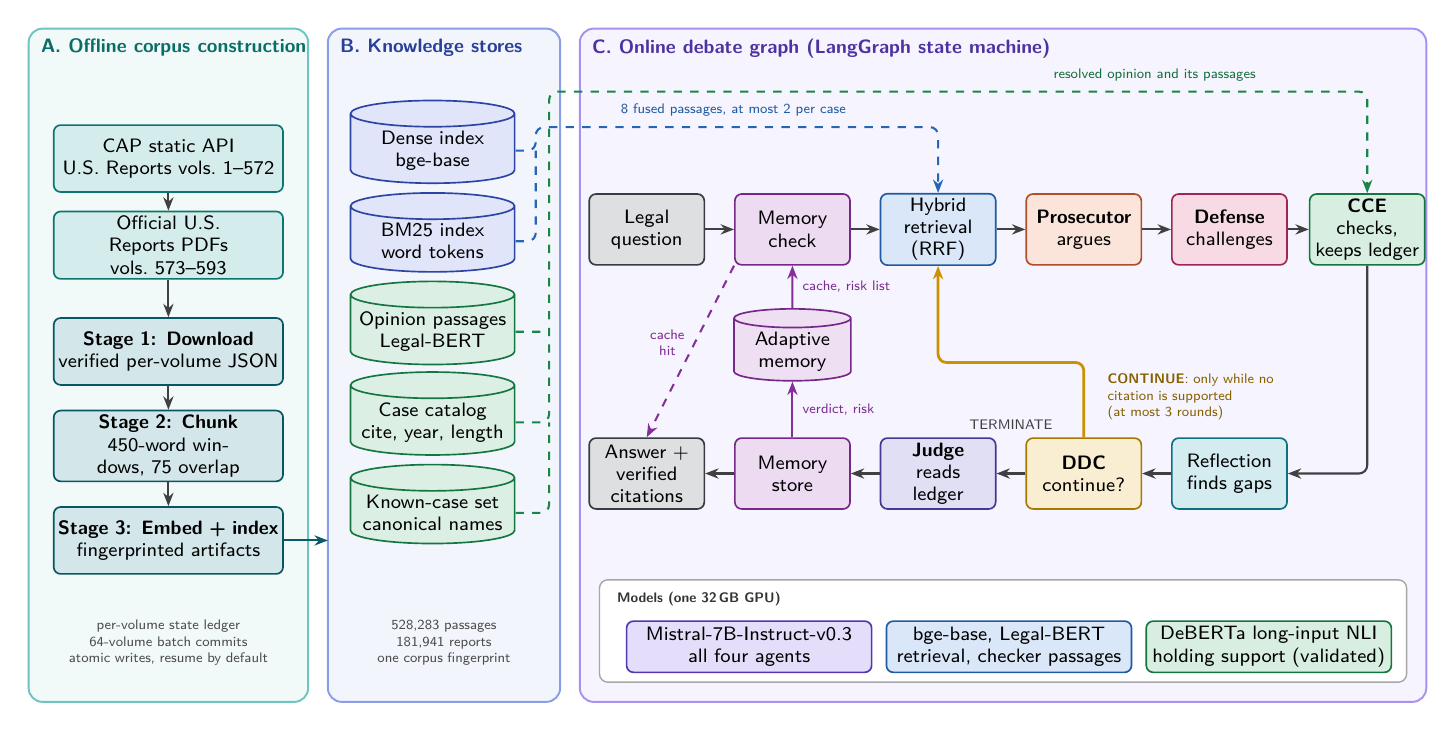
\begin{tikzpicture}[
    x=1cm, y=1cm,
    font=\sffamily\scriptsize,
    >={Stealth[length=1.7mm,width=1.3mm]},
    lane/.style={draw=#1!60, fill=#1!6, rounded corners=5pt, line width=0.7pt},
    lanetitle/.style={font=\sffamily\bfseries\scriptsize, text=#1!70!black, anchor=north west, inner sep=2pt},
    blk/.style={draw=#1!75!black, fill=#1!18, rounded corners=2.5pt, align=center, line width=0.6pt,
                minimum height=9mm, inner sep=1.6pt, text width=13.5mm},
    wide/.style={blk=#1, text width=28mm, minimum height=8.5mm},
    store/.style={cylinder, shape border rotate=90, aspect=0.16, draw=#1!75!black, fill=#1!16, line width=0.6pt,
                  align=center, text width=20mm, minimum height=10.5mm, inner sep=1.2pt},
    flow/.style={->, line width=0.75pt, draw=black!75},
    bus/.style={->, line width=0.75pt, draw=#1!85!black, dashed, rounded corners=3pt},
    note/.style={font=\sffamily\tiny, text=black!70, align=center},
]
% ── lanes ───────────────────────────────────────────────────────────────────
\draw[lane=cData]   (0.00,0.55) rectangle (3.55,9.10);
\draw[lane=cStore]  (3.80,0.55) rectangle (6.75,9.10);
\draw[lane=cAgent]  (7.00,0.55) rectangle (17.75,9.10);
\node[lanetitle=cData]  at (0.08,9.05) {A. Offline corpus construction};
\node[lanetitle=cStore] at (3.88,9.05) {B. Knowledge stores};
\node[lanetitle=cAgent] at (7.08,9.05) {C. Online debate graph (LangGraph state machine)};

% ── lane A ──────────────────────────────────────────────────────────────────
\node[wide=cData] (cap) at (1.775,7.45) {CAP static API\\U.S.\ Reports vols.\ 1--572};
\node[wide=cData] (pdf) at (1.775,6.35) {Official U.S.\ Reports PDFs\\vols.\ 573--593};
\node[wide=cPipe] (s1)  at (1.775,5.00) {\textbf{Stage 1: Download}\\verified per-volume JSON};
\node[wide=cPipe] (s2)  at (1.775,3.80) {\textbf{Stage 2: Chunk}\\450-word windows, 75 overlap};
\node[wide=cPipe] (s3)  at (1.775,2.60) {\textbf{Stage 3: Embed + index}\\fingerprinted artifacts};
\node[note, text width=31mm] at (1.775,1.30) {per-volume state ledger\\64-volume batch commits\\atomic writes, resume by default};
\draw[flow] (cap.south) -- (pdf.north);
\draw[flow] (pdf.south) -- (s1.north);
\draw[flow] (s1.south) -- (s2.north);
\draw[flow] (s2.south) -- (s3.north);

% ── lane B ──────────────────────────────────────────────────────────────────
\node[store=cStore, minimum height=9mm] (dense) at (5.13,7.55) {Dense index\\bge-base};
\node[store=cStore, minimum height=9mm] (bm25)  at (5.13,6.40) {BM25 index\\word tokens};
\node[store=cVerify, minimum height=9mm] (lb) at (5.13,5.25) {Opinion passages\\Legal-BERT};
\node[store=cVerify, minimum height=9mm] (cat)  at (5.13,4.10) {Case catalog\\cite, year, length};
\node[store=cVerify, minimum height=9mm] (known) at (5.13,2.95) {Known-case set\\canonical names};
\node[note, text width=26mm] at (5.275,1.30) {\ResCorpusChunks\ passages\\\ResCorpusReports\ reports\\one corpus fingerprint};
\draw[flow, draw=cPipe!80!black] (s3.east) -- (3.80,2.60);

% ── lane C: debate graph ────────────────────────────────────────────────────
\def\ra{6.55}\def\rb{3.45}
\node[blk=cUser]   (q)    at (7.85,\ra)  {Legal\\question};
\node[blk=cMemory] (mc)   at (9.70,\ra)  {Memory\\check};
\node[blk=cRetr]   (ret)  at (11.55,\ra) {Hybrid\\retrieval\\(RRF)};
\node[blk=cPros]   (pro)  at (13.40,\ra) {\textbf{Prosecutor}\\argues};
\node[blk=cDef]    (def)  at (15.25,\ra) {\textbf{Defense}\\challenges};
\node[blk=cVerify] (cce)  at (17.00,\ra) {\textbf{CCE}\\checks,\\keeps ledger};
\node[blk=cUser]   (ans)  at (7.85,\rb)  {Answer +\\verified\\citations};
\node[blk=cMemory] (ms)   at (9.70,\rb)  {Memory\\store};
\node[blk=cJudge]  (jud)  at (11.55,\rb) {\textbf{Judge}\\reads\\ledger};
\node[blk=cCtrl]   (ddc)  at (13.40,\rb) {\textbf{DDC}\\continue?};
\node[blk=cRefl]   (ref)  at (15.25,\rb) {Reflection\\finds gaps};
\node[store=cMemory, text width=14mm, minimum height=9mm] (mem) at (9.70,5.00) {Adaptive\\memory};

\draw[flow] (q) -- (mc);
\draw[flow] (mc) -- (ret);
\draw[flow] (ret) -- (pro);
\draw[flow] (pro) -- (def);
\draw[flow] (def) -- (cce);
\draw[flow, rounded corners=3pt] (cce.south) |- (ref.east);
\draw[flow] (ref) -- (ddc);
\draw[flow] (ddc) -- (jud);
\node[note, text=black!75] at (12.475,4.07) {TERMINATE};
\draw[flow] (jud) -- (ms);
\draw[flow] (ms) -- (ans);
\draw[flow, draw=cCtrl!90!black, line width=1pt, rounded corners=3pt] (ddc.north) -- ++(0,0.95) -| (ret.south);
\node[note, text=cCtrl!60!black, text width=30mm, align=left, anchor=west] at (13.58,4.42) {\textbf{CONTINUE}: only while no\\citation is supported\\(at most 3 rounds)};
\draw[flow, draw=cMemory!85!black] (mem) -- node[right, note, text=cMemory!80!black] {cache, risk list} (mc);
\draw[flow, draw=cMemory!85!black] (ms) -- node[right, note, text=cMemory!80!black] {verdict, risk} (mem);
\draw[flow, draw=cMemory!85!black, dashed] (mc.south west) -- node[left, note, text=cMemory!80!black, pos=0.45] {cache\\hit} (ans.north);

% ── data buses from the stores ──────────────────────────────────────────────
\draw[bus=cRetr]   (dense.east) -- (6.44,7.55) -- (6.44,7.85) -- (11.55,7.85) -- (ret.north);
\draw[bus=cRetr, -] (bm25.east) -- (6.44,6.40) -- (6.44,7.55);
\draw[bus=cVerify] (cat.east) -- (6.61,4.10) -- (6.61,8.30) -- (17.00,8.30) -- (cce.north);
\draw[bus=cVerify, -] (lb.east) -- (6.61,5.25);
\draw[bus=cVerify, -] (known.east) -- (6.61,2.95) -- (6.61,4.10);
\node[note, text=cRetr!75!black, anchor=south] at (8.95,7.86) {8 fused passages, at most 2 per case};
\node[note, text=cVerify!70!black, anchor=south] at (14.30,8.31) {resolved opinion and its passages};

% ── models strip ────────────────────────────────────────────────────────────
\draw[draw=black!35, fill=white, rounded corners=3pt, line width=0.5pt] (7.25,0.80) rectangle (17.50,2.10);
\node[note, anchor=west, text=black!80] at (7.35,1.85) {\textbf{Models (one 32\,GB GPU)}};
\node[blk=cAgent, text width=30mm, minimum height=6.5mm] at (9.15,1.25) {Mistral-7B-Instruct-v0.3\\all four agents};
\node[blk=cRetr,  text width=30mm, minimum height=6.5mm] at (12.45,1.25) {bge-base, Legal-BERT\\retrieval, checker passages};
\node[blk=cVerify,text width=30mm, minimum height=6.5mm] at (15.75,1.25) {DeBERTa long-input NLI\\holding support (validated)};
\end{tikzpicture}

\caption{Architecture of the final \sys\ system. Lane~A builds the corpus offline in three resumable stages. Lane~B holds the resulting stores. Lane~C is the debate graph: solid arrows are control flow, dashed arrows are data read from the stores, and the amber arrow is the loop taken when the controller requests another round.}\label{fig:arch}
\end{figure*}

% ════════════════════════════════════════════════════════════════════════════
\section{Related Work}\label{sec:related}

\subsection{Domain-Specific Legal Language Models}
Early mitigation relied on domain adaptation. DISC-LawLLM fine-tunes a general model on a supervised legal corpus built around syllogistic prompting and adds a retrieval module~\cite{disclawllm}; LawGPT injects Chinese legal knowledge through pre-training and instruction tuning~\cite{lawgpt}; Lawformer extends the context window for long legal documents~\cite{lawformer}. Progress is tracked by LegalBench~\cite{legalbench}, LawBench~\cite{lawbench}, LexGLUE~\cite{lexglue} and LegalAgentBench~\cite{legalagentbench}. Fine-tuning shifts the output distribution toward legally plausible phrasing. It does not add a mechanism that separates plausible text from verified text, and a fine-tuned model still completes a query at the edge of its training distribution with an authority that conforms to the style of the jurisdiction.

\subsection{Retrieval-Augmented Generation for Legal Text}
RAG conditions generation on passages retrieved from an external corpus~\cite{lewis2020}. Corrective RAG grades the retrieved documents and triggers corrective retrieval when their quality is insufficient~\cite{crag}; HyPA-RAG adapts retrieval parameters to query complexity for legal and policy text~\cite{hyparag}; agentic search extends retrieval into multi-step legal reasoning~\cite{lras}. Legal relevance is neither purely lexical nor purely semantic: a statute number or a party name must match exactly, whereas a controlling precedent may share no vocabulary with the question. Hybrid retrieval therefore combines BM25~\cite{bm25} with dense retrieval over legal embeddings such as Legal-BERT~\cite{legalbert}, and merges the two rankings by reciprocal rank fusion (RRF), which requires no score calibration~\cite{rrf}. Hybrid strategies are reported to outperform single-modality retrieval for legal case retrieval~\cite{sectionhybrid} and for graph-augmented legal question answering~\cite{leakgraphrag}. Measured hallucination rates of deployed legal RAG tools~\cite{magesh2025} nevertheless show that correct retrieval does not ensure correct use of the retrieved text.

\subsection{Post-Generation Detection and Symbolic Constraints}
SelfCheckGPT detects hallucination from the disagreement among stochastic samples of one model~\cite{selfcheckgpt}; Chain-of-Verification has the model draft and answer verification questions about its own output~\cite{cove}; Self-RAG trains a model to emit reflection tokens that trigger retrieval and self-critique~\cite{selfrag}. In each method the verifier shares its parameters with the generator, so a systematic error is reproduced consistently and passes the check. External structure removes that dependence. HalluGraph aligns knowledge graphs extracted from the context and from the response and reports entity grounding and relation preservation, with an area under the curve near 0.98 on structured control documents and near 0.89 on generative legal tasks~\cite{hallugraph}. Falkor-IRAC constrains generation with an issue-rule-analysis-conclusion graph of Indian judgments and gives a verifier agent authority to reject an output that has no supporting path~\cite{falkorirac}. Both systems audit a single generation pass; a rejected output is discarded, not refined.

\subsection{Multi-Agent Debate}
Debate among several model instances improves factuality and reasoning~\cite{du2024}. Agents with conflicting roles counteract premature consensus, termed degeneration of thought~\cite{liang2024}, although the gains depend strongly on the debate configuration~\cite{smit2024}. General frameworks such as MetaGPT~\cite{metagpt} and AutoGen~\cite{autogen} provide cooperative role orchestration. In the legal domain, ChatLaw routes a query through cooperating specialised agents over a knowledge-graph-enhanced mixture of experts~\cite{chatlaw}; no agent is assigned to contest another agent's claims. AgentCourt simulates court proceedings with adversarial lawyer agents that evolve through accumulated experience~\cite{agentcourt}. PROClaim casts claim verification as courtroom deliberation with progressive retrieval during the debate and reports 81.7\% accuracy on Check-COVID, of which progressive retrieval contributes 7.5 percentage points~\cite{proclaim}; it targets biomedical claims, uses proprietary models, and keeps no state between queries.

\subsection{Positioning}
Table~\ref{tab:related} summarises the structural properties of the most closely related systems. Role specialisation, entity-level verification against a corpus, and adversarial debate with iterative retrieval have each been demonstrated separately. As far as we could find, no existing system verifies citations inside the debate loop, and none keeps citation-level memory across queries. We designed \sys\ to fill that gap using open models and commodity hardware.

\begin{table}[t]
\caption{Structural comparison with related systems}\label{tab:related}
\centering
\footnotesize
\setlength{\tabcolsep}{2.6pt}
\begin{tabular}{@{}lccccc@{}}
\toprule
System & \shortstack{Adversarial\\debate} & \shortstack{In-loop\\citation\\check} & \shortstack{Hybrid\\retrieval} & \shortstack{Cross-\\query\\memory} & \shortstack{Open\\models} \\
\midrule
ChatLaw~\cite{chatlaw}            & \no  & \no & \yes      & \no       & \yes \\
HalluGraph~\cite{hallugraph}      & \no  & \no & \no       & \no       & \yes \\
LeAK-GraphRAG~\cite{leakgraphrag} & \no  & \no & \yes      & \no       & \yes \\
Falkor-IRAC~\cite{falkorirac}     & \no  & \no & \no       & \no       & \yes \\
AgentCourt~\cite{agentcourt}      & \yes & \no & \no       & \partialy & \yes \\
PROClaim~\cite{proclaim}          & \yes & \no & \partialy & \no       & \no  \\
\midrule
\textbf{\sys\ (this work)}        & \yes & \yes & \yes     & \yes      & \yes \\
\bottomrule
\end{tabular}
\end{table}

% ════════════════════════════════════════════════════════════════════════════
\section{System Overview}
Fig.~\ref{fig:arch} shows the architecture of the final system. An offline pipeline (lane A) turns the source volumes into the knowledge stores of lane B: the retrieval indexes, a case catalog and a set of canonical case names, all tied to a single corpus fingerprint. At query time a LangGraph state machine (lane C) runs the debate. A state object carries the question, the retrieved passages, the arguments and citations of both sides, the citation report, the reflection output and the controller's decision. Each node reads the state and returns an update.

A query first passes a memory check. If the memory already holds a verdict for the same question, that verdict is returned without a debate; otherwise the citations previously found unreliable are attached to the state. Hybrid retrieval then supplies passages. The prosecutor argues for an answer, and the defense challenges it using counter-evidence that it retrieves independently. The Citation Confidence Engine (CCE) checks every citation from both sides. A reflection agent lists the gaps that remain and proposes follow-up queries, and the Dynamic Debate Controller (DDC) either starts another round with those queries or hands over to the judge. The judge may rest its answer only on citations the CCE marked as supported. Finally, the verdict and the citation risk observed during the debate are written to memory. Several of these components changed between our first and our final system: the rule for matching a stored verdict, the support test of the CCE, the way verified citations are kept across rounds, the controller's stopping rule, and the retriever. Section~\ref{sec:method} describes the original design, and Sections~\ref{sec:repairs} and~\ref{sec:remaining} describe each change and the reason for it.

% ════════════════════════════════════════════════════════════════════════════
\section{Corpus Construction}

\subsection{Sources}
Our primary source is the Caselaw Access Project (CAP)~\cite{cap}, which publishes the United States Reports as one metadata file and one JSON document per case for each volume. We targeted volumes 1 to \ResCorpusVolumesTarget. CAP covers volumes 1 to \ResCorpusVolumesCap. For volumes 573 to 593 we extracted the opinions ourselves from the bound volumes and preliminary prints published by the Supreme Court~\cite{usreports}. Our parser reads each PDF page by page, classifies running heads to locate case boundaries, restores ligatures from glyph identifiers, and moves footnotes to the end of the opinion. We validated it against CAP on volume 572, where it found all 27 opinions at the same starting page. Volumes 594 to \ResCorpusVolumesTarget\ have no published opinion text in either source. We record them as unavailable instead of skipping them silently.

\subsection{Staged, Resumable Ingestion}
We split ingestion into three stages that share no in-memory state. Stage~1 only downloads, Stage~2 only chunks and never touches the network, and Stage~3 only embeds and indexes. Each stage keeps a ledger with one state per volume (Fig.~\ref{fig:pipeline}) and commits a positional checkpoint after every \ResCorpusCheckpointInterval\ volumes. Ledgers and artifacts are written atomically: the content goes to a temporary file, is flushed to disk, and is then renamed over the target. A stage resumes by default. On every run it re-reads each artifact, checks its schema version, status and content hash, and reprocesses only the volumes whose artifact is missing or invalid. A chunk file also records the hash of the raw volume it was derived from, so it is invalidated whenever that hash changes.

Stage~3 computes a fingerprint over the ordered chunk identifiers and metadata. The corpus file, the lexical index, the known-case set, the case catalog and the embedding checkpoint each store that fingerprint, so an index built from one corpus cannot be combined with another by mistake. If the corpus grows and the previous corpus is an unchanged prefix, only the new passages are embedded. We never delete existing data without an explicit overwrite instruction.

\begin{figure}[t]
\centering
% Fig. 2 - per-volume state machine of the staged ingestion pipeline (column width, drawn at natural size).
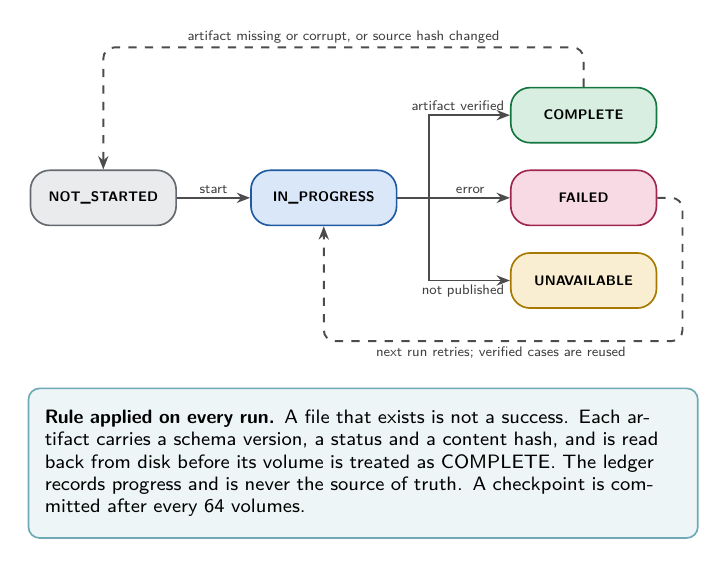
\begin{tikzpicture}[
    x=1cm, y=1cm,
    font=\sffamily\scriptsize,
    >={Stealth[length=1.7mm,width=1.3mm]},
    st/.style={draw=#1!75!black, fill=#1!18, rounded corners=7pt, align=center, line width=0.6pt,
               minimum height=7mm, minimum width=18.5mm, inner sep=2pt, font=\sffamily\tiny\bfseries},
    tr/.style={->, line width=0.7pt, draw=black!70},
    lbl/.style={font=\sffamily\tiny, text=black!75, align=center, inner sep=1.2pt},
]
\node[st=cNeutral] (ns) at (0.00,2.60) {NOT\_STARTED};
\node[st=cRetr]    (ip) at (2.80,2.60) {IN\_PROGRESS};
\node[st=cVerify]  (ok) at (6.10,3.65) {COMPLETE};
\node[st=cDef]     (fl) at (6.10,2.60) {FAILED};
\node[st=cCtrl]    (na) at (6.10,1.55) {UNAVAILABLE};

\draw[tr] (ns) -- node[lbl, above] {start} (ip);
\draw[tr] (ip.east) -- ++(0.40,0) |- (ok.west);
\draw[tr] (ip) -- (fl);
\draw[tr] (ip.east) -- ++(0.40,0) |- (na.west);
\node[lbl, anchor=south east] at (5.14,3.66) {artifact verified};
\node[lbl, anchor=south] at (4.66,2.61) {error};
\node[lbl, anchor=north east] at (5.14,1.54) {not published};
% between runs: an invalid artifact sends a COMPLETE volume back; a FAILED volume is retried
\draw[tr, dashed, rounded corners=4pt] (ok.north) -- ++(0,0.50) -| (ns.north);
\node[lbl, anchor=south] at (3.05,4.51) {artifact missing or corrupt, or source hash changed};
\draw[tr, dashed, rounded corners=4pt] (fl.east) -- ++(0.32,0) -- ++(0,-1.82) -| (ip.south);
\node[lbl, anchor=north] at (5.05,0.76) {next run retries; verified cases are reused};

\draw[draw=cPipe!60, fill=cPipe!7, rounded corners=4pt, line width=0.6pt] (-0.95,-1.72) rectangle (7.55,0.18);
\node[font=\sffamily\scriptsize, align=left, anchor=west, text width=80mm, inner sep=0pt] at (-0.75,-0.77) {%
\textbf{Rule applied on every run.} A file that exists is not a success. Each artifact carries a schema version, a status and a content hash, and is read back from disk before its volume is treated as COMPLETE. The ledger records progress and is never the source of truth. A checkpoint is committed after every \ResCorpusCheckpointInterval\ volumes.};
\end{tikzpicture}

\caption{State of one volume in a pipeline stage. Dashed transitions occur between runs.}\label{fig:pipeline}
\end{figure}

\subsection{Chunking, Indexing and the Case Catalog}
We split each case into windows of 450 words with an overlap of 75 words. A chunk inherits the case name, year, court, volume, reporter and first page of its parent, and it records the parent identifier and its word offsets. We embed the passages with Legal-BERT~\cite{legalbert} and store them in a persistent ChromaDB collection~\cite{chroma}, and we build a BM25 index over the same passages.

The case catalog lists every report in the corpus with its name, reporter citation, year, number of chunks and number of words. We classify a report of fewer than 300 words as an order entry (for example, a one-line denial of certiorari) and do not treat it as an opinion. The verifier needs this distinction, because the name of a landmark decision usually also appears in several order entries, while a holding can only be checked against the opinion. Table~\ref{tab:corpus} gives the corpus statistics.

\begin{table}[t]
\caption{Corpus statistics}\label{tab:corpus}
\centering
\footnotesize
\begin{tabular}{@{}lr@{}}
\toprule
Quantity & Value \\
\midrule
Target volumes of the United States Reports & \ResCorpusVolumesTarget \\
Volumes indexed & \ResCorpusVolumes \\
\quad from the CAP static API & \ResCorpusVolumesCap \\
\quad from official Supreme Court PDFs & \ResCorpusVolumesPdf \\
Volumes without published opinion text & \ResCorpusVolumesUnavailable \\
Volumes failed & \ResCorpusFailedVolumes \\
Case documents (CAP / official PDFs) & \ResCorpusCasesCap\ / \ResCorpusCasesPdf \\
Reports in the case catalog & \ResCorpusReports \\
\quad opinions ($\geq 300$ words) & \ResCorpusOpinions \\
\quad order entries ($< 300$ words) & \ResCorpusOrders \\
Passages (450 words, 75 overlap) & \ResCorpusChunks \\
Decision years & \ResCorpusYearFirst--\ResCorpusYearLast \\
Dense index on disk & \ResCorpusIndexGB\ GB \\
\bottomrule
\end{tabular}
\end{table}

% ════════════════════════════════════════════════════════════════════════════
\section{Method}\label{sec:method}

\subsection{Hybrid Retrieval}
This section describes the system as we first built it; the later changes are described where they were made. For a query $q$, the dense retriever returns the four passages nearest to the Legal-BERT embedding of $q$, and the lexical retriever returns the four passages with the highest BM25 score. The two rankings are merged by reciprocal rank fusion~\cite{rrf}:
\begin{equation}
\mathrm{RRF}(d) = \sum_{m \in \{\mathrm{dense},\,\mathrm{BM25}\}} \frac{1}{k + \mathrm{rank}_m(d)}, \qquad k = 60,
\end{equation}
and at most eight fused passages are passed to the debate. An entity map from case names and reporter citations to the retrieved passages is built for each round. In rounds after the first, the query is extended with up to two follow-up queries issued by the reflection agent, so that the evidence pool changes while the debate is in progress.

\subsection{Debate Agents}
All agents are instances of Mistral-7B-Instruct-v0.3~\cite{mistral7b} with role-specific system prompts and are required to return a JSON object.

The \emph{prosecutor} argues an answer to the question from the retrieved passages. Its prompt restricts citations to cases present in the retrieved context and lists the citations that memory marks as high risk. Each citation is returned with a case name, a reporter cite and the holding it is cited for.

The \emph{defense} is evidence-disjoint. Counter-queries are generated deterministically from the question and from the prosecutor's citations and holdings, and the passages they retrieve exclude every passage the prosecutor received. The defense returns challenges, a counter-argument, its own citations, a challenge strength in $[0,1]$ and a concession flag. The share of defense citations that merely repeat the prosecutor's evidence is recorded as the evidence overlap ratio.

The \emph{reflection} agent reads the exchange, lists propositions that neither side has supported, and emits follow-up queries.

The \emph{judge} receives the debate and the citation confidence report of the last round and returns a verdict, the citations relied on, the citations considered uncertain and a self-assessed confidence. A citation named by the judge that the CCE did not mark as supported is removed from the verified list by the program, not by the prompt.

\subsection{Citation Confidence Engine}\label{sec:cce}
The CCE scores each citation $c = (n, r, h)$, where $n$ is the case name, $r$ the reporter cite and $h$ the asserted holding, in the order shown in Fig.~\ref{fig:cce}.

\emph{Existence.} $E(c) = 1$ if $n$ equals a canonical name in the corpus. Otherwise $E$ is the best fuzzy similarity between $n$ and a canonical name. In a catalog of this size a loose match exists for almost any name, so a fuzzy match is retained only if both party names agree with the candidate or the character-level similarity is at least 0.85.

\emph{Resolution.} The pair $(n, r)$ is resolved to one report in the case catalog. If the report printed at the cited volume and page carries the cited name, the cite is confirmed and $E = 1$. If the name only resembles a real case and the cite belongs to a different case, the citation as given does not exist and $E = 0$. When several reports share the name, the opinion is preferred over order entries.

\emph{Verdict without support.} If $E < 0.85$ the citation is labelled \textsc{fabricated} when the cited volume lies within the corpus, and \textsc{unverifiable} otherwise. A real case whose opinion text is not in the corpus is \textsc{unverifiable}. No support score is computed in these cases.

\emph{Support.} For an existing case with an opinion, the three passages of \emph{that opinion} most similar to the embedding of $h$ are selected through a metadata filter on the parent document. The selected text is divided into units $w_1,\dots,w_J$ and scored by a cross-encoder for natural-language inference:
\begin{align}
S(c) &= \max_{1 \leq j \leq J} \; P_{\mathrm{NLI}}\!\left(\text{entailment} \mid w_j,\, h\right), \\
\mathrm{CCS}(c) &= E(c) \cdot S(c).
\end{align}

\emph{First version.} In our first evaluation the units were overlapping windows of 450 characters, the model was a small DeBERTa-v3 cross-encoder~\cite{debertav3}, and the tier was \textsc{supported} if $S \geq 0.70$, \textsc{uncertain} if $0.40 \leq S < 0.70$, and \textsc{misattributed} if $S < 0.40$. We had validated neither the model nor the thresholds on labelled citations.

\emph{Repaired version.} The repaired checker (Fig.~\ref{fig:cce}) reports two verdicts for each citation. The existence verdict is one of \emph{exists}, \emph{not found} and \emph{not in corpus}. The support verdict is computed by a model, a passage selection and a threshold $\tau_g$ that are named in a gate file. The gate file is written by a validation experiment (Section~\ref{sec:validation}) and opens the gate only if the selected model separates correct from incorrect holdings on held-out citations with an area under the ROC curve of at least \ResGateRequiredAUC. With the gate open, a citation is \textsc{supported} if $S \geq \tau_g$, \textsc{misattributed} if the model assigns a contradiction probability of at least 0.90 to one of the units, and \textsc{not shown} otherwise. The last tier states that the passages read do not show the holding; it does not state that the citation is wrong. With the gate closed, an existing citation is labelled \textsc{verified} with $\mathrm{CCS} = E$, and no support verdict reaches the judge, the controller or the memory. In both versions a citation whose holding is supported but whose reporter cite belongs to another case is capped at \textsc{uncertain}.

The order of these steps is the central design decision. A verifier that retrieves evidence by case name alone compares the holding with whichever passage happens to carry that name, and in this corpus that is often an order entry or an unrelated passage. Resolving the citation to its opinion first removes that failure. We measure its effect in Section~\ref{sec:stress}.

\begin{figure}[t]
\centering
% Fig. 3 - decision procedure of the Citation Confidence Engine (column width, drawn at natural size).
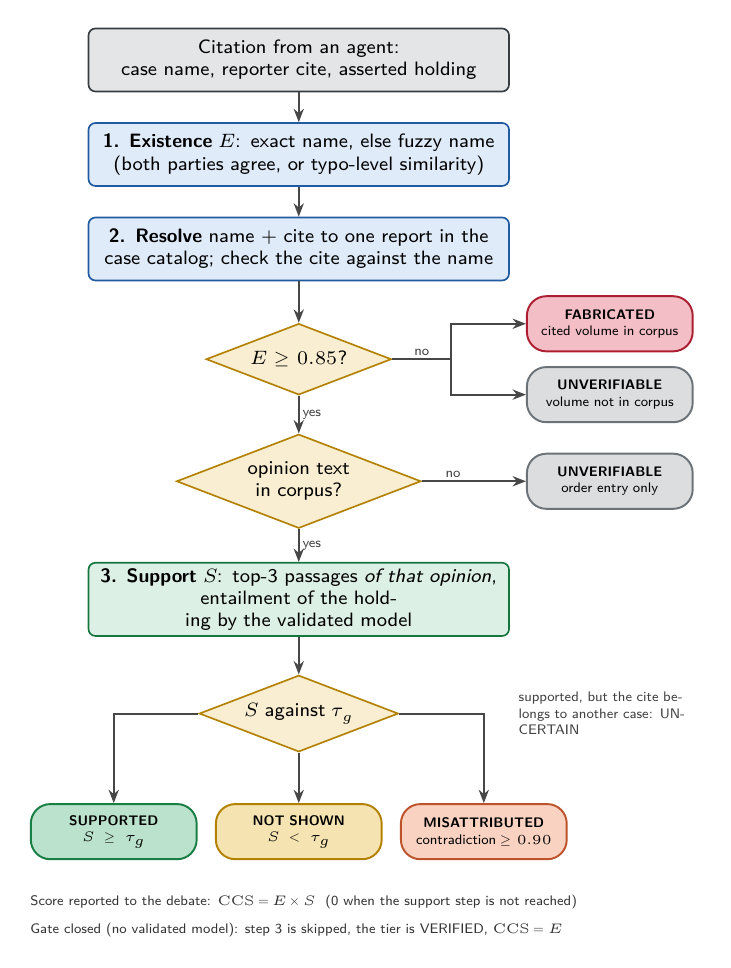
\begin{tikzpicture}[
    x=1cm, y=1cm,
    font=\sffamily\scriptsize,
    >={Stealth[length=1.7mm,width=1.3mm]},
    proc/.style={draw=#1!75!black, fill=#1!15, rounded corners=2.5pt, align=center, line width=0.6pt,
                 minimum height=8mm, text width=52mm, inner sep=2pt},
    test/.style={draw=cCtrl!80!black, fill=cCtrl!18, diamond, aspect=2.6, align=center, line width=0.6pt, inner sep=0.5pt, text width=17mm},
    out/.style={draw=#1!80!black, fill=#1!30, rounded corners=7pt, align=center, line width=0.7pt,
                minimum height=7mm, text width=20mm, inner sep=1.5pt, font=\sffamily\tiny},
    fl/.style={->, line width=0.7pt, draw=black!72},
    lbl/.style={font=\sffamily\tiny, text=black!75, inner sep=1pt},
]
\node[proc=cUser]   (in)  at (-0.90,9.75) {Citation from an agent:\\case name, reporter cite, asserted holding};
\node[proc=cRetr]   (ex)  at (-0.90,8.55) {\textbf{1. Existence} $E$: exact name, else fuzzy name\\(both parties agree, or typo-level similarity)};
\node[proc=cRetr]   (rs)  at (-0.90,7.35) {\textbf{2. Resolve} name + cite to one report in the\\case catalog; check the cite against the name};
\node[test]         (t1)  at (-0.90,5.95) {$E \geq 0.85$?};
\node[test]         (t2)  at (-0.90,4.40) {opinion text\\in corpus?};
\node[proc=cVerify] (nli) at (-0.90,2.90) {\textbf{3. Support} $S$: top-3 passages \emph{of that opinion},\\entailment of the holding by the validated model};
\node[test]         (t3)  at (-0.90,1.45) {$S$ against $\tau_g$};

\node[out=cFab]     (fab) at (3.05,6.40) {\textbf{FABRICATED}\\cited volume in corpus};
\node[out=cNeutral] (unv) at (3.05,5.50) {\textbf{UNVERIFIABLE}\\volume not in corpus};
\node[out=cNeutral] (un2) at (3.05,4.40) {\textbf{UNVERIFIABLE}\\order entry only};
\node[out=cVerify]  (sup) at (-3.25,-0.05) {\textbf{SUPPORTED}\\$S \geq \tau_g$};
\node[out=cCtrl]    (unc) at (-0.90,-0.05) {\textbf{NOT SHOWN}\\$S < \tau_g$};
\node[out=cPros]    (mis) at (1.45,-0.05) {\textbf{MISATTRIBUTED}\\contradiction $\geq 0.90$};

\draw[fl] (in) -- (ex);
\draw[fl] (ex) -- (rs);
\draw[fl] (rs) -- (t1);
\draw[fl] (t1) -- node[lbl, right] {yes} (t2);
\draw[fl] (t2) -- node[lbl, right] {yes} (nli);
\draw[fl] (nli) -- (t3);
\draw[fl] (t1.east) -- node[lbl, above, pos=0.5] {no} ++(0.75,0) |- (fab.west);
\draw[fl] (t1.east) -- ++(0.75,0) |- (unv.west);
\draw[fl] (t2.east) -- node[lbl, above, pos=0.3] {no} (un2.west);
\draw[fl] (t3.south) -- (unc.north);
\draw[fl] (t3.west) -| (sup.north);
\draw[fl] (t3.east) -| (mis.north);
\node[lbl, text width=23mm, align=left, anchor=west, text=black!75] at (1.85,1.45) {supported, but the cite belongs to another case: UNCERTAIN};
\node[lbl, anchor=west, text=black!80] at (-4.35,-0.95) {Score reported to the debate: $\mathrm{CCS} = E \times S$ \ (0 when the support step is not reached)};
\node[lbl, anchor=west, text=black!80] at (-4.35,-1.30) {Gate closed (no validated model): step 3 is skipped, the tier is VERIFIED, $\mathrm{CCS} = E$};
\end{tikzpicture}

\caption{Decision procedure of the repaired Citation Confidence Engine. Existence and cite resolution precede the support test, support is computed only against the opinion the citation resolves to, and the support test is used only when a support model has passed validation.}\label{fig:cce}
\end{figure}

\subsection{Dynamic Debate Controller}
After each round $t$ the controller reads the mean score $\overline{\mathrm{CCS}}_t$, the minimum score $\mathrm{CCS}^{\min}_t$, the gap list $G_t$ of the reflection agent, the challenge strength $\sigma_t$ and the concession flag. With $W_t = [\overline{\mathrm{CCS}}_t < 0.60] \lor [\mathrm{CCS}^{\min}_t < 0.40]$ denoting weak citations, the debate continues if and only if
\begin{equation}
t < T_{\max} \;\land\; \lnot\,\mathrm{concede}_t \;\land\; |G_t| \geq 1 \;\land\; \bigl(W_t \lor \sigma_t > 0.5\bigr),
\end{equation}
with $T_{\max} = 3$ rounds. The minimum is included so that a single unsupported citation cannot be hidden by a favourable mean. Weak citations without any identified gap terminate the debate, since no follow-up query is available.

\subsection{Adaptive Memory}\label{sec:memory}
Memory consists of two vector collections keyed by Legal-BERT embeddings. The \emph{verdict cache} stores the final answer of each debate. In the first version a new query whose cosine similarity to a stored query exceeds 0.92 is answered from the cache, and only the answer text is restored. In the repaired version a stored verdict is returned only for the same question, compared after lower-casing and removal of punctuation and surplus white space, and the citations and the confidence of the stored verdict are restored with the answer. The \emph{citation-risk index} stores, for every citation labelled \textsc{fabricated}, \textsc{misattributed} or \textsc{unverifiable}, a running mean of its CCS. At the start of a debate the five risk entries nearest to the query are retrieved, and those with a mean score below 0.45 are passed to the prosecutor and the defense as citations to avoid.

\subsection{Verification-Grounded Confidence}
We tie the confidence reported with a verdict to the verification outcome, and not to the judge's self-assessment alone. Let $V$ be the set of verified citations the judge relies on, $U$ the set of citations it lists as uncertain, $\overline{\mathrm{CCS}}_V$ the mean score over $V$, and $\gamma$ the self-assessed confidence. Then
\begin{equation}
\mathrm{conf} =
\begin{cases}
0.7\,\overline{\mathrm{CCS}}_V + 0.3\,\gamma, & |V| > 0,\\
\min(\gamma,\, 0.35), & |V| = 0,\ |U| > 0,\\
\min(\gamma,\, 0.20), & |V| = |U| = 0.
\end{cases}
\end{equation}
As a result, an answer that rests on no verified citation cannot be reported with high confidence, however the model rates itself.

% ════════════════════════════════════════════════════════════════════════════
\section{First Evaluation}\label{sec:first}
This section reports our first evaluation exactly as we ran and recorded it. Section~\ref{sec:audit} then explains which of these results do not mean what they appear to mean.

\subsection{Implementation}
We implemented the system in Python with LangGraph~\cite{langgraph}, ChromaDB and PyTorch, and ran all experiments on one workstation with an Intel Core Ultra~9 285K processor, 127\,GB of memory and one NVIDIA RTX~5090 GPU with 32\,GB of memory. The generator is loaded in 16-bit floating point and sampled at temperature 0.1 with at most 1024 new tokens. Table~\ref{tab:params} lists the parameters.

\begin{table}[t]
\caption{Parameters. Rows marked ``first'', ``repaired'' and ``second step'' differ between the versions of the system; all other rows are fixed.}\label{tab:params}
\centering
\footnotesize
\begin{tabular}{@{}llr@{}}
\toprule
Component & Parameter & Value \\
\midrule
Chunking & window / overlap (words) & 450 / 75 \\
Retrieval & dense top-$k$ / BM25 top-$k$ & 4 / 4 \\
\quad second step & candidates per ranking / per-case limit & 8 / 2 \\
 & RRF constant $k$ & 60 \\
CCE & existence threshold & 0.85 \\
 & passages of the opinion read & 3 \\
\quad first & supported / uncertain from & 0.70 / 0.40 \\
 & NLI window / stride (characters) & 450 / 350 \\
\quad repaired & validation area required to open the gate & \ResGateRequiredAUC \\
 & support threshold $\tau_g$ (from the gate file) & \ResGateThreshold \\
 & contradiction probability for misattributed & 0.90 \\
DDC & maximum rounds $T_{\max}$ & 3 \\
 & mean / minimum CCS to continue & 0.60 / 0.40 \\
 & challenge-strength threshold & 0.5 \\
\quad second step & stop once a citation is supported & yes \\
Memory & high-risk mean CCS & 0.45 \\
\quad first & verdict cache: cosine similarity above & 0.92 \\
\quad repaired & verdict cache: same question & exact \\
Generator & temperature / new tokens & 0.1 / 1024 \\
\bottomrule
\end{tabular}
\end{table}

\subsection{Test Set}
Our benchmark consists of \ResTestCasesAll\ questions on United States constitutional and federal law, each paired with a target decision and a reference holding. We keep a question only if the corpus contains enough source text of its target decision to evaluate an answer, which we define as the target resolving in the case catalog to an opinion of at least 500 words. \ResTestCasesExcluded\ questions do not meet this condition and are excluded, which leaves \ResTestCases. One of the excluded targets is represented in the corpus only by order entries, because its volume is incomplete at the source; the other three were decided in volumes that have no published opinion text. A question may draw on opinions from any number of volumes. Only the absence of the target opinion excludes it.

\subsection{Baseline}
The baseline is a single-agent RAG system that uses the same generator, the same hybrid retriever and the same corpus. The four highest-ranked passages, each truncated to 300 characters, are placed in one prompt and the model is asked for an answer with case citations. No defense, verification, controller or memory is present.

\subsection{Measures of the First Evaluation}
All measures are computed per question and averaged. Let $C$ be the set of distinct case names cited by any agent in a debate.
\begin{itemize}
\item \emph{Fabricated-name rate} (HR): the fraction of $C$ with no canonical name in the corpus at fuzzy similarity of at least 85.
\item \emph{Answer semantic similarity} (ASS): cosine similarity between the Legal-BERT embeddings of the final answer and the reference holding.
\item \emph{Authority recall} (AR): 1 if the target decision is in $C$, else 0. \emph{Authority precision} (AP): AR divided by $|C|$.
\item \emph{Misattribution rate} (MAR) and \emph{holding-attribution accuracy} (HAA): the fractions of scored citations labelled \textsc{misattributed} and \textsc{supported} by the CCE.
\item \emph{Unsupported-claim rate} (UCR): the fraction of citations the judge rejected.
\item \emph{Debate convergence rate} (DCR): the fraction of debates that end in a concession or with confidence of at least 0.70.
\end{itemize}
We test differences between the two systems with a paired bootstrap over questions ($10^4$ resamples), and we report proportions in the stress test with 95\% Wilson intervals.

\subsection{Design of the Citation Stress Test}
We test the verifier in isolation on \ResStressTotal\ citations with known labels: (i) the \ResStressCorrectN\ target decisions with their reference holdings (\emph{correct}); (ii) the same decisions with the holding of a different benchmark question (\emph{holding swapped}); (iii) \ResStressCaseholdN\ of the target decisions paired with hand-written false statements of law that contradict settled doctrine (\emph{false-holding distractors}); (iv) \ResStressFabCiteN\ invented case names with a reporter cite inside the corpus; (v) \ResStressFabNoCiteN\ invented names without a cite; and (vi) the \ResStressOffCorpusN\ real decisions whose opinions are outside the corpus. Only type (i) should be accepted. A citation counts as accepted when its tier is \textsc{supported}.

\subsection{Ablation Variants}
Four variants each remove one component from the graph: A1 removes the defense node; A2 removes the CCE, so that the judge relies on its own citations and its own confidence; A3 removes the memory nodes; A4 replaces the controller by termination after one round. Each variant is run on all \ResTestCases\ questions with a separate, initially empty memory.

\subsection{Debate System Against the Baseline, as Recorded}
Table~\ref{tab:main} gives the recorded comparison. The fabricated-name rate is \ResLexHR\% for \sys\ and \ResBaseHR\% for the baseline; the difference of \ResDiffHR\pp\ (interval [\ResDiffHRLow, \ResDiffHRHigh]\pp) is not significant. \ResLexFlagged\ of \ResLexCites\ distinct citations were flagged for \sys\ and \ResBaseFlagged\ of \ResBaseCites\ for the baseline. Manual inspection shows that the measure over-counts: all three names flagged for the baseline, and one of the three flagged for \sys, are real decisions written with additional text such as an appended reporter cite.

The baseline is recorded as significantly better on answer similarity (\ResDiffASS, interval [\ResDiffASSLow, \ResDiffASSHigh]) and on authority precision (\ResDiffAP\pp, interval [\ResDiffAPLow, \ResDiffAPHigh]\pp); the difference in authority recall (\ResDiffAR\pp, interval [\ResDiffARLow, \ResDiffARHigh]\pp) is not significant. \sys\ returned an answer without any citation in \ResLexNoCiteAnswers\ of \ResTestCases\ cases against \ResBaseNoCiteAnswers\ for the baseline. Of the \ResTestCases\ debates, \ResLexRoundsOne\ are recorded with one round and \ResLexRoundsMax\ with the maximum of \ResLexMaxRounds; the judge's confidence is bimodal, with \ResLexConfLow\ debates at or below 0.20 and \ResLexConfHigh\ at or above 0.70, and a mean of \ResLexConf.

\begin{table}[t]
\caption{First evaluation, as recorded: debate system against the single-agent baseline on \ResTestCases\ questions. $\Delta$ is \sys\ minus baseline with a 95\% paired-bootstrap interval. Section~\ref{sec:audit} qualifies every row.}\label{tab:main}
\centering
\footnotesize
\setlength{\tabcolsep}{3.2pt}
\begin{tabular}{@{}lrrrl@{}}
\toprule
Measure & \sys & Baseline & $\Delta$ & 95\% interval \\
\midrule
HR (\%) $\downarrow$ & \ResLexHR & \ResBaseHR & \ResDiffHR\ResDiffHRMark & [\ResDiffHRLow, \ResDiffHRHigh] \\
ASS $\uparrow$ & \ResLexASS & \ResBaseASS & \ResDiffASS\ResDiffASSMark & [\ResDiffASSLow, \ResDiffASSHigh] \\
AR (\%) $\uparrow$ & \ResLexAR & \ResBaseAR & \ResDiffAR\ResDiffARMark & [\ResDiffARLow, \ResDiffARHigh] \\
AP (\%) $\uparrow$ & \ResLexAP & \ResBaseAP & \ResDiffAP\ResDiffAPMark & [\ResDiffAPLow, \ResDiffAPHigh] \\
Citations per answer & \ResLexCitesPerAnswer & \ResBaseCitesPerAnswer & & \\
Answers without citation & \ResLexNoCiteAnswers & \ResBaseNoCiteAnswers & & \\
\midrule
\multicolumn{5}{@{}l}{\emph{Measures defined only for the debate}} \\
MAR (\%) & \ResLexMAR & & & \\
HAA (\%) & \ResLexHAA & & & \\
UCR (\%) & \ResLexUCR & & & \\
Mean judge confidence & \ResLexConf & & & \\
DCR (\%) & \ResLexDCR & & & \\
Mean rounds per debate & \ResLexRoundsMean & & & \\
\bottomrule
\multicolumn{5}{@{}l}{$^{\ast}$ interval excludes zero.}
\end{tabular}
\end{table}

\subsection{Results of the Citation Stress Test}\label{sec:stress}
Table~\ref{tab:stress} and Fig.~\ref{fig:stress} report the behaviour of the first version of the CCE on labelled citations. The test does not involve the debate, and the audit leaves its results unchanged. No invented citation was accepted. Every invented citation with a reporter cite inside the corpus was labelled \textsc{fabricated}, and every invented citation without a cite, like every real decision outside the corpus, was labelled \textsc{unverifiable}; the verifier does not call a decision fabricated when it lacks the means to check it. Of the citations whose holding was swapped, \ResStressMisattrAccepted\ of \ResStressMisattrN\ (\ResStressMisattrAcceptedPct\%) were accepted, and none of the false-holding distractors. In total \ResStressFalseAccepts\ of \ResStressWrongTotal\ incorrect citations were accepted, a rejection rate of \ResStressWrongRejectedPct\%.

The cost is recall. Only \ResStressCorrectAccepted\ of \ResStressCorrectN\ correct citations (\ResStressCorrectAcceptedPct\%, interval [\ResStressCorrectAcceptedLow, \ResStressCorrectAcceptedHigh]\%) were accepted, and \ResStressCorrectMisattributed\ were labelled \textsc{misattributed}. The support score separates correct from swapped holdings with an area under the ROC curve of \ResStressAUC.

\emph{Effect of opinion resolution.} Table~\ref{tab:cceorder} compares the verifier with its predecessor, which retrieved evidence by case name without resolving the citation to a report. Resolution raised the acceptance of correct citations from \ResStressOldCorrectAcceptedPct\% to \ResStressCorrectAcceptedPct\%, raised the share of invented citations with a cite that are labelled \textsc{fabricated} from \ResStressOldFabCiteFabricated\ of \ResStressOldFabCiteN\ to \ResStressFabCiteFabricated\ of \ResStressFabCiteN, and removed the acceptance of invented names without a cite (\ResStressOldFabNoCiteAccepted\ of \ResStressOldFabNoCiteN\ before, \ResStressFabNoCiteAccepted\ after).

\emph{Evidence selection.} To locate the cause of the low recall, we repeated the support step on the correct and the swapped citations with different selections of passages from the resolved opinion: the nearest passages in embedding space, the passages with the highest BM25 score within the opinion, a rank fusion of both, and the entire opinion.
\ifnum\ResEvidenceComplete=0
\textbf{[The evidence-selection study has not been run.]}
\fi
With three or five passages, between \ResEvFewCorrectMin\ and \ResEvFewCorrectMax\ of the \ResEvCorrectTotal\ correct citations are accepted, whichever ranking selects the passages, and between \ResEvFewSwappedMin\ and \ResEvFewSwappedMax\ of the swapped ones. Reading the entire opinion raises acceptance of correct citations to \ResEvWholeCorrect\ (\ResEvWholeCorrectPct\%), but \ResEvWholeSwapped\ swapped holdings (\ResEvWholeSwappedPct\%) are then accepted as well. With this entailment model, recall is obtained only together with false acceptance; the choice of passages does not remove the limit. Section~\ref{sec:validation} shows that the choice of model does.

\begin{table}[t]
\caption{Citation stress test of the first checker: tier assigned, by citation type}\label{tab:stress}
\centering
\footnotesize
\setlength{\tabcolsep}{2.4pt}
\begin{tabular}{@{}lrrrrrrr@{}}
\toprule
Citation type & $n$ & \rotatebox{70}{Supported} & \rotatebox{70}{Uncertain} & \rotatebox{70}{Misattrib.} & \rotatebox{70}{Fabricated} & \rotatebox{70}{Unverif.} & \shortstack{Accepted\\(\%)} \\
\midrule
Correct & \ResStressCorrectN & \ResStressCorrectSupported & \ResStressCorrectUncertain & \ResStressCorrectMisattributed & \ResStressCorrectFabricated & \ResStressCorrectUnverifiable & \ResStressCorrectAcceptedPct \\
Holding swapped & \ResStressMisattrN & \ResStressMisattrSupported & \ResStressMisattrUncertain & \ResStressMisattrMisattributed & \ResStressMisattrFabricated & \ResStressMisattrUnverifiable & \ResStressMisattrAcceptedPct \\
False-holding distractor & \ResStressCaseholdN & \ResStressCaseholdSupported & \ResStressCaseholdUncertain & \ResStressCaseholdMisattributed & \ResStressCaseholdFabricated & \ResStressCaseholdUnverifiable & \ResStressCaseholdAcceptedPct \\
Invented, with cite & \ResStressFabCiteN & \ResStressFabCiteSupported & \ResStressFabCiteUncertain & \ResStressFabCiteMisattributed & \ResStressFabCiteFabricated & \ResStressFabCiteUnverifiable & \ResStressFabCiteAcceptedPct \\
Invented, no cite & \ResStressFabNoCiteN & \ResStressFabNoCiteSupported & \ResStressFabNoCiteUncertain & \ResStressFabNoCiteMisattributed & \ResStressFabNoCiteFabricated & \ResStressFabNoCiteUnverifiable & \ResStressFabNoCiteAcceptedPct \\
Real, outside corpus & \ResStressOffCorpusN & \ResStressOffCorpusSupported & \ResStressOffCorpusUncertain & \ResStressOffCorpusMisattributed & \ResStressOffCorpusFabricated & \ResStressOffCorpusUnverifiable & \ResStressOffCorpusAcceptedPct \\
\bottomrule
\end{tabular}
\end{table}

\begin{table}[t]
\caption{Effect of resolving the citation to its opinion before the support test}\label{tab:cceorder}
\centering
\footnotesize
\setlength{\tabcolsep}{3.5pt}
\begin{tabular}{@{}lrr@{}}
\toprule
Outcome & \shortstack{Evidence by\\case name} & \shortstack{Evidence from the\\resolved opinion} \\
\midrule
Correct citations accepted & \ResStressOldCorrectAccepted/\ResStressOldCorrectN & \ResStressCorrectAccepted/\ResStressCorrectN \\
Swapped holdings accepted & \ResStressOldMisattrAccepted/\ResStressOldMisattrN & \ResStressMisattrAccepted/\ResStressMisattrN \\
Invented with cite, labelled fabricated & \ResStressOldFabCiteFabricated/\ResStressOldFabCiteN & \ResStressFabCiteFabricated/\ResStressFabCiteN \\
Invented without cite, accepted & \ResStressOldFabNoCiteAccepted/\ResStressOldFabNoCiteN & \ResStressFabNoCiteAccepted/\ResStressFabNoCiteN \\
\bottomrule
\end{tabular}
\end{table}

\begin{figure}[t]
\centering
% Fig. 5 - verdicts of the citation checker by citation type (column width).
\begin{tikzpicture}
\begin{axis}[
    xbar stacked, width=0.74\columnwidth, height=5.4cm,
    bar width=8pt, enlarge y limits=0.11,
    xmin=0, xmax=100, xtick={0,25,50,75,100},
    xlabel={share of citations of that type (\%)},
    ytick={0,1,2,3,4,5}, y dir=reverse,
    yticklabels={{Correct ($n$=\ResStressCorrectN)},{Holding swapped ($n$=\ResStressMisattrN)},{False-holding distractor ($n$=\ResStressCaseholdN)},{Invented, with cite ($n$=\ResStressFabCiteN)},{Invented, no cite ($n$=\ResStressFabNoCiteN)},{Real, outside corpus ($n$=\ResStressOffCorpusN)}},
    y tick label style={font=\sffamily\scriptsize, align=right},
    x tick label style={font=\sffamily\scriptsize}, xlabel style={font=\sffamily\scriptsize},
    xmajorgrids, grid style={black!12}, axis line style={black!45}, tick style={black!45},
    legend style={font=\sffamily\tiny, draw=none, fill=none, at={(0.20,1.03)}, anchor=south, legend columns=3, /tikz/every even column/.append style={column sep=5pt}},
    legend image code/.code={\draw[#1, draw=none] (0cm,-0.08cm) rectangle (0.24cm,0.10cm);},
]
\addplot[fill=cVerify,  draw=white, line width=0.5pt] table[x=supported,     y=row] {generated/stress_verdicts.dat};
\addplot[fill=cCtrl,    draw=white, line width=0.5pt] table[x=uncertain,     y=row] {generated/stress_verdicts.dat};
\addplot[fill=cPros,    draw=white, line width=0.5pt] table[x=misattributed, y=row] {generated/stress_verdicts.dat};
\addplot[fill=cFab,     draw=white, line width=0.5pt] table[x=fabricated,    y=row] {generated/stress_verdicts.dat};
\addplot[fill=cNeutral, draw=white, line width=0.5pt] table[x=unverifiable,  y=row] {generated/stress_verdicts.dat};
\legend{Supported,Uncertain,Misattributed,Fabricated,Unverifiable}
\end{axis}
\end{tikzpicture}

\caption{Tier assigned by the first version of the CCE to each type of citation in the stress test. Only citations of the first type should be labelled supported.}\label{fig:stress}
\end{figure}

\subsection{Ablation, as Recorded}
\ifnum\ResAblationComplete=0
\textbf{[The ablation summary on disk covers \ResAblationCases\ cases per variant; the values below are not final.]}
\fi
Table~\ref{tab:ablation} gives the recorded ablation. The runner saved one mean per measure and variant, so no interval is available. Removing memory (A3) raised mean confidence from \ResAblFullConf\ to \ResAblAThreeConf, and terminating after one round (A4) left confidence (\ResAblAFourConf) and answer similarity (\ResAblAFourASS) at the level of the full system at \ResAblAFourMinutes\ instead of \ResAblFullMinutes\ minutes. The fabricated-name rates of all variants lie between \ResAblHRMin\% and \ResAblHRMax\%. The last column of the table is taken from the audit and is explained in the next section.

\begin{table}[t]
\caption{First ablation, as recorded, on \ResAblationCases\ questions per variant. The last column, from the audit of the run logs, counts the questions that were answered from the verdict cache without a debate.}\label{tab:ablation}
\centering
\footnotesize
\setlength{\tabcolsep}{3.0pt}
\begin{tabular}{@{}llrrrrr@{}}
\toprule
 & Removed & \shortstack{Fabr.\\name\\rate (\%)} & \shortstack{Answer\\simi-\\larity} & \shortstack{Judge\\confi-\\dence} & \shortstack{Run\\time\\(min)} & \shortstack{Debates\\skipped} \\
\midrule
Full & none & \ResAblFullHR & \ResAblFullASS & \ResAblFullConf & \ResAblFullMinutes & \ResAudCacheAblFull \\
A1 & defense agent & \ResAblAOneHR & \ResAblAOneASS & \ResAblAOneConf & \ResAblAOneMinutes & \ResAudCacheAblAOne \\
A2 & verifier (CCE) & \ResAblATwoHR & \ResAblATwoASS & \ResAblATwoConf & \ResAblATwoMinutes & \ResAudCacheAblATwo \\
A3 & adaptive memory & \ResAblAThreeHR & \ResAblAThreeASS & \ResAblAThreeConf & \ResAblAThreeMinutes & \ResAudCacheAblAThree \\
A4 & controller (one round) & \ResAblAFourHR & \ResAblAFourASS & \ResAblAFourConf & \ResAblAFourMinutes & \ResAudCacheAblAFour \\
\bottomrule
\end{tabular}
\end{table}

% ════════════════════════════════════════════════════════════════════════════
\section{Audit of the First Evaluation}\label{sec:audit}
Taken at face value, the first evaluation says that the debate adds cost and no benefit. Before accepting that conclusion we went back through the saved result files, the run logs and the code. We did not repeat any experiment or change any result file. Where a question could not be answered from the files alone, we added a deterministic diagnostic that makes no call to the generator. The audit produced five findings.

\subsection{The Verdict Cache Replaced a Third of the Debates}
The first thing we noticed was a pattern in the benchmark run. \ResAudCacheBench\ of the \ResTestCases\ cases show the signature of a debate that never happened: a confidence of 0, a single round and no citation. They are exactly the \ResLexNoCiteAnswers\ answers recorded without a citation, and exactly the \ResLexRoundsOne\ debates recorded with one round. The logs of the ablation runs show the cause directly. In each variant with memory, between \ResAudCacheAblMin\ and \ResAudCacheAblMax\ questions were answered from the verdict cache, and in the variant without memory none were (Table~\ref{tab:ablation}).

Our benchmark contains no repeated question, so every one of these cache hits returned the answer to a different question. The reason is that Legal-BERT was never trained for sentence similarity, and its embeddings of legal questions sit very close to one another. Of the \ResAudCollisionPairsTotal\ pairs of benchmark questions, \ResAudCollisionPairs\ exceed our threshold of 0.92, and \ResAudCollisionQuestions\ questions have an earlier question above it. Separating all of them would have required a threshold of \ResAudNoCollisionThreshold. We were able to reproduce each of the \ResAudCacheAblFull\ hits in the logged run of the full system from the question embeddings alone, and the two questions shared a target decision in \ResAudCacheSameTarget\ of them. A cache hit restored only the answer text, which is why the confidence stayed at zero and the citation list stayed empty.

This single defect accounts for several of the results in Section~\ref{sec:first}: every answer without a citation, every ``one-round'' debate, \ResAudCacheBench\ of the \ResLexConfLow\ debates with a confidence at or below 0.20, and the recorded deficit in authority recall. It also explains what had looked like an effect of removing memory. Removing memory simply removed the skipped debates. Over the debates that actually took place, the mean confidence is \ResAudImpliedConfFull\ in the full system and \ResAudImpliedConfAThree\ without memory.

\subsection{The Debated Cases Tell a Different Story}
If we look only at the \ResAudDebated\ cases that were actually debated, the picture reverses. There \sys\ cited the target decision in \ResAudDebatedLexAR\% of cases, against \ResAudDebatedBaseAR\% for the baseline (interval of the difference [\ResAudDebatedARLow, \ResAudDebatedARHigh]\pp, \ResAudDebatedARP). We treat this number with caution. The subset is not a random sample, since a case is skipped precisely when its question lies close to an earlier one, so the figure is an indication and not an estimate. It was, however, the reason we decided to measure the debate again without the cache (Section~\ref{sec:postaudit}).

\subsection{Two Measures Do Not Measure What They Name}
Authority precision, as we had defined it, is simply authority recall divided by the number of citations. We checked that this identity holds for every case of both systems. The measure therefore drops whenever an answer cites more than one case, and it can never detect an incorrect citation. The deficit recorded for the debate reflects nothing more than the fact that it cites more cases per answer.

Answer semantic similarity turned out to have almost no usable range. When we score the reference holding of a \emph{different} benchmark case with the same Legal-BERT embeddings, it obtains \ResAudSimFloor\ on average, and the question itself, returned as if it were the answer, obtains \ResAudSimQuestion. The recorded values of \ResLexASS\ and \ResBaseASS\ therefore sit in a narrow band that starts at \ResAudSimFloor, and simply restating the question scores about as well as answering it.

\subsection{The Verifier Was Not Validated, and the Debate Depends on It}
The support score of our first checker separates correct from swapped holdings with an AUC of only \ResStressAUC, and it rejects most correct citations (Section~\ref{sec:stress}). This matters because three other components act on its verdict. The judge may rely only on supported citations, so a correct citation that the checker rejects can never appear in the answer. The controller keeps a debate going while citation scores are weak, which is why all \ResAudDebatedAtMaxRounds\ debated cases of the benchmark run went to the maximum number of rounds. The risk index of the memory stores rejected citations as citations to avoid. On top of this, each round overwrites the citations and the citation report of the round before it. In the variant without memory, \ResAudAThreeSupportedAny\ of \ResAudAThreeDebates\ debates contained a supported citation in some round, but in \ResAudAThreeSupportLost\ of them no supported citation was left by the final round, which is the only one the judge reads.

\subsection{The Protocol Could Not Support Its Conclusions}
Finally, the protocol itself left little room for checking anything. Generation was sampled, and we had set no seed. The benchmark run saved one scorecard per case and the ablation saved one mean per variant. We kept no answers, citation lists or retrieved passages, so no result could be inspected afterwards. The baseline issued a different dense query from the debate (the question alone instead of the question with its jurisdiction) and read four passages of 300 characters, whereas the prosecutor reads eight of 500. In the first ablation run, the switch that disables the checker had not been declared in the state schema of the graph, and the framework silently dropped it. The A2 row of Table~\ref{tab:ablation} comes from the run we repeated after fixing this, and we keep the invalid result in the archive.

% ════════════════════════════════════════════════════════════════════════════
\section{Repairs}\label{sec:repairs}
We made the repairs in two steps. The first step consists of four repairs. Each one addresses a specific finding of the audit, and we did not choose any of them for its effect on the benchmark scores.
\begin{enumerate}
\item \emph{Seeded, traced runs.} Question $i$ of a run with seed $s$ is generated with seed $100003\,s + i$. For every question we now save the retrieved passages, the parsed and the raw output of every agent in every round, the citation report of every round, the controller's decisions, the judge's output, and whether the cache answered. A run resumes after an interruption and never overwrites a saved case.
\item \emph{Same-question verdict cache.} The cache answers only when the normalised question is the same, and it restores the citations and the confidence together with the answer (Section~\ref{sec:memory}). In the evaluation runs it is either switched off or, in the run that fills the memory for Section~\ref{sec:cachetest}, unable to answer because the questions are distinct. No debate was skipped in any post-audit run.
\item \emph{Measures that state what they count.} The measures of Section~\ref{sec:postaudit} replace authority precision and Legal-BERT similarity. A skipped debate is treated as a category of its own and is never scored as an answer.
\item \emph{Existence and support reported separately, behind a gate.} The checker of Section~\ref{sec:cce} now states whether a citation exists independently of whether its holding is supported. The support verdict steers the judge, the controller and the memory only if a support model has passed validation.
\end{enumerate}
We left the other defects found by the audit untouched in this first step: the risk index of the memory, the overwriting of citations and reports from round to round together with the judge's restriction to the last report, the continuation rule of the controller, and the Legal-BERT retriever. They are therefore part of what the runs of Section~\ref{sec:postaudit} measure. Those runs then told us which of these defects were worth repairing in a second step (Section~\ref{sec:remaining}).

% ════════════════════════════════════════════════════════════════════════════
\section{Evaluation of the Repaired System}\label{sec:postaudit}

\subsection{Protocol}
\emph{Configurations.} We run eight configurations on the \ResTestCases\ questions in this section and five more in Section~\ref{sec:remaining}. Two are baselines that differ only in context: four passages of 300 characters, as in the first evaluation, and eight passages of 500 characters, which is what the prosecutor receives. Both issue the same dense query as the debate. The \emph{first debate, cache off} is the system of the first evaluation with its original checker and with memory removed, so that no debate is skipped. It provides the measurement that the first evaluation could not. The \emph{repaired debate} uses the validated checker. Variants A1 to A4 each remove one component from the repaired debate. We ran the baselines and the first debate with three seeds. The repaired debate has two seeds and its variants one, because we stopped their remaining repeats once the second step of repairs had turned the repaired debate into an intermediate system. Every table states the number of seeds behind its values.

\emph{Correction of the baseline's citations.} We ask the baseline to return its citations as a list of objects. In \ResParseBaseFourChanged\ of \ResParseBaseFourAnswers\ four-passage answers and in \ResParseBaseEightChanged\ of \ResParseBaseEightAnswers\ eight-passage answers, the model returned a list of plain strings instead. Our parser, which we had carried over from the first evaluation, kept only objects, so each of those answers was recorded as citing nothing. We found the error after all runs were complete, when we traced the surprisingly high share of eight-passage answers without a citation back to the raw outputs. Because every run saves the model's raw output, we could read the citations again from it without repeating a run, and we keep the files as originally saved. The correction raises the share of baseline answers that rest on the target from \ResParseBaseFourTargetAsSaved\% to \ResPaBaseFourTargetAnswer\% with four passages and from \ResParseBaseEightTargetAsSaved\% to \ResPaBaseEightTargetAnswer\% with eight. All baseline values reported after Table~\ref{tab:ablation} use the corrected reading. The baseline of the first evaluation (Table~\ref{tab:main}) was scored with the same parser and is understated by an amount we cannot determine, since its outputs were not saved. The debate agents wrote objects in every call we examined, so the debate values are unaffected.

\emph{Measures.} We resolve every citation through the case catalog. \emph{Target cited by the answer} is 1 if a citation that the final answer rests on resolves to the target decision. For the debate these are the citations the judge relies on, and for the baseline they are the citations of its answer. \emph{Target cited by any agent} is 1 if any citation made by any agent in any round resolves to the target. We report the \emph{number of citations} next to these measures and never divide it into them. An \emph{answer on no existing authority} rests on no citation that resolves to a report. A \emph{citation to a non-existent case} names a case that is not in the catalog even though the cited volume is in the corpus. \emph{Support shown} is the share of checked citations of the final round that are labelled \textsc{supported}. \emph{Answer similarity} is the cosine similarity between sentence embeddings~\cite{sbert} of the answer and of the reference holding, computed with a model trained for sentence similarity (all-mpnet-base-v2~\cite{mpnet}). As reference points, the holding of a different case obtains \ResPaSimFloor\ on average and the question itself obtains \ResPaSimQuestion.

\emph{Statistics.} All comparisons are paired by question. When a configuration has several seeds, the value of a question is its mean over the seeds. We report 95\% percentile intervals from $10^4$ bootstrap resamples of questions and $p$-values from a two-sided sign-flip permutation test with $10^4$ permutations. We call a difference significant only if $p < 0.05$ and the interval excludes zero. We apply no correction for multiple comparisons. The comparisons are few, and we report all of them.

\subsection{Validation of the Support Model}\label{sec:validation}
We split the labelled citations of the stress test (\ResStressCorrectN\ correct, \ResStressMisattrN\ with a swapped holding and \ResStressCaseholdN\ with a false holding) once, with a fixed seed, into a development half and a test half. The test half holds \ResGateTestSetCorrect, \ResGateTestSetSwapped\ and \ResGateTestSetFalse\ citations of the three kinds. We then scored \ResGateCandidates\ candidates: five entailment cross-encoders, each with windows of 450 characters and with whole passages as units, and the generator itself asked for a yes-or-no judgement on whole passages, each combined with three ways of selecting passages from the cited opinion. We fixed the selection rule before looking at any score. The candidate with the highest development AUC is selected, its threshold is the one that maximises the difference between true and false acceptance on the development half, and the gate opens only if that candidate reaches an AUC of at least \ResGateRequiredAUC\ on the test half.

Table~\ref{tab:verifier} lists the best candidate of each model. The four cross-encoders trained on sentence-level inference data reach test AUCs between \ResGateOtherTestAUCMin\ and \ResGateOtherTestAUCMax, and the model and configuration of our first evaluation reach \ResGateFirstModelTestAUC. The rule selected a cross-encoder trained for long inputs~\cite{tasksource} that reads whole passages. Its development AUC is \ResGateDevAUC\ and its test AUC is \ResGateTestAUC\ (interval [\ResGateTestAUCLow, \ResGateTestAUCHigh]). On the test half it accepted \ResGateTestCorrect\ correct citations, \ResGateTestSwapped\ swapped holdings and \ResGateTestFalse\ false holdings. The gate therefore opened, with $\tau_g = \ResGateThreshold$. The generator used as a verifier reached the same development AUC, and the rule resolved the tie in favour of the cross-encoder, which had been scored first. We would not have adopted the generator in any case. The checker cannot yet load it as a support model, and this test cannot tell us whether its judgement on a landmark decision comes from the passage or from what the model already knows about the case.

\emph{Near-miss holdings.} The swapped holdings in this test come from arbitrary other cases, which makes them relatively easy to reject. As a harder probe, which we ran after the gate was fixed and which had no influence on it, we paired each target decision with the reference holding of the \emph{most similar} other benchmark case. The validated model accepted \ResProbeCorrect\ of \ResProbeN\ correct holdings, \ResProbeUnrelated\ holdings of unrelated cases and \ResProbeNearMiss\ near-miss holdings (\ResProbeNearMissPct\%). The last figure is an upper bound on the error, because an opinion often restates the holding of a closely related case. It still shows that a \textsc{supported} verdict does not rule out a holding that really belongs to a neighbouring decision.

\begin{table}[t]
\caption{Validation of the support model: best candidate of each model by development area. Acceptance is on the test half (\ResGateTestSetCorrect\ correct, \ResGateTestSetSwapped\ swapped, \ResGateTestSetFalse\ false holdings). Bold: the candidate selected by the fixed rule.}\label{tab:verifier}
\centering
\footnotesize
\setlength{\tabcolsep}{2.4pt}
\begin{tabular}{@{}>{\raggedright\arraybackslash}p{2.35cm}>{\raggedright\arraybackslash}p{1.35cm}rrrrr@{}}
\toprule
Model & Units; passages & \shortstack{Dev.\\area} & \shortstack{Test\\area} & \shortstack{Correct\\acc.} & \shortstack{Swapped\\acc.} & \shortstack{False\\acc.} \\
\midrule
\ResRowsVerifier
\bottomrule
\end{tabular}
\end{table}

\subsection{Retrieval}
Table~\ref{tab:retrieval} reports, for each retriever on its own and for two fusions, how many of the \ResRetQuestions\ questions have a passage of the target opinion among the first one, four and eight results. The dense retriever of our system places the target among its four results for only \ResRetDenseTopFour\ questions (\ResRetDenseTopFourPct\%), whereas the lexical retriever does so for \ResRetLexicalTopFour\ (\ResRetLexicalTopFourPct\%). A general-purpose embedding model trained for retrieval~\cite{bge} reaches \ResRetBgeTopFour. In hindsight this is not surprising: Legal-BERT is a masked language model with no retrieval objective, yet it supplies half of the eight passages a debate receives. The deployed fusion contains the target among its eight passages for \ResRetSystemTopEight\ questions and ranks it first for \ResRetSystemRankOne; the best fusion we tested reaches \ResRetBestTopEight\ and \ResRetBestRankOne. Since we picked that fusion on the same questions, the finding here is the ranking of the configurations and not its best number. We did not change retrieval for the repaired debate of this section, so for \ResRetSystemMissEight\ of the \ResRetQuestions\ questions the target opinion is missing from the first-round passages.

\begin{table}[t]
\caption{Retrieval: number of the \ResRetQuestions\ questions with a passage of the target opinion among the first $k$ results}\label{tab:retrieval}
\centering
\footnotesize
\setlength{\tabcolsep}{3.5pt}
\begin{tabular}{@{}>{\raggedright\arraybackslash}p{5.2cm}rrr@{}}
\toprule
Retriever & $k=1$ & $k=4$ & $k=8$ \\
\midrule
\ResRowsRetrieval
\bottomrule
\end{tabular}
\end{table}

\subsection{Debate Against the Baselines}
Table~\ref{tab:pamain} and Fig.~\ref{fig:pamain} give the measures, and Table~\ref{tab:padiff} gives the paired differences.

\emph{The first debate without the cache.} Once no debate is skipped, the first system cites the target decision somewhere in the debate in \ResPaOldTargetAny\% of cases, compared with \ResPaBaseFourTargetAny\% for the four-passage baseline (\cmp{OldBaseFour}{TargetAny}{\pp}). Its answers, however, rest on the target in only \ResPaOldTargetAnswer\% of cases (\cmp{OldBaseFour}{TargetAnswer}{\pp}), and \ResPaOldNoAuthority\% of them rest on no existing authority at all. The gap of \ResPaOldFoundNotUsed\ percentage points between what the agents cite and what the answer uses is the effect of the first checker on the judge.

\emph{The repaired debate.} With the validated checker, the answers rest on the target in \ResPaFullTargetAnswer\% of cases (\cmp{FullOld}{TargetAnswer}{\pp}), and the share of answers on no existing authority falls to \ResPaFullNoAuthority\% (\cmp{FullOld}{NoAuthority}{\pp}). How often the target is cited somewhere in the debate does not change (\ResPaFullTargetAny\% against \ResPaOldTargetAny\%, \ResCmpFullOldTargetAnyP). In other words, the repair changes what the judge is allowed to use, not what the agents find.

\emph{Against the baselines.} The repair does not carry the debate past a single agent. In answers resting on the target, the difference between the repaired debate and the four-passage baseline is \cmpword{FullBaseFour}{TargetAnswer} (\cmp{FullBaseFour}{TargetAnswer}{\pp}). Against the eight-passage baseline, which reads the same context as the prosecutor, the debate is behind (\cmp{FullBaseEight}{TargetAnswer}{\pp}). The two baselines do not differ significantly from each other (\cmp{BaseEightBaseFour}{TargetAnswer}{\pp}, eight passages minus four). The debate also leaves more answers on no existing authority than the four-passage baseline (\cmp{FullBaseFour}{NoAuthority}{\pp}), and the answers of both debate configurations are less similar to the reference holding than those of both baselines (repaired debate against four passages: \cmp{FullBaseFour}{Sim}{}). We note that the similarity measure remains coarse, since a restatement of the question would score \ResPaSimQuestion. What the debate does retain is breadth. Its agents cite the target somewhere more often than the four-passage baseline does (\cmp{FullBaseFour}{TargetAny}{\pp}).

\emph{Existence and cost.} No citation that a debate answer rests on names a non-existent case. The agents of the first debate did cite \ResPaOldNotFound\ such cases among \ResPaOldCitationsMade\ citations, but the checker kept them out of the answers. The four-passage baseline cited none. The eight-passage baseline cited \ResPaBaseEightNotFoundAnswerCount\ among \ResPaBaseEightAnswerCitations, and all of them appear in its answers (Table~\ref{tab:pamain}). In the final round of the repaired debate, \ResPaFullSupportShown\% of the \ResPaFullSupportChecked\ checked citations are labelled \textsc{supported}. A repaired debate takes \ResPaFullSecondsPerCase\,s per question, against \ResPaBaseFourSecondsPerCase\,s for a baseline, which is about \ResPaFullTimeRatio\ times as long, and every debate ran the maximum number of rounds (mean \ResPaFullRounds).

\begin{table}[t]
\caption{Post-audit runs on \ResTestCases\ questions, earlier retrieval: mean over the seeds of each configuration. Baseline citations as read from the raw outputs. ``No authority'' abbreviates no existing authority.}\label{tab:pamain}
\centering
\footnotesize
\setlength{\tabcolsep}{2.6pt}
\begin{tabular}{@{}lrrrr@{}}
\toprule
Measure & \shortstack{Baseline\\4 pass.} & \shortstack{Baseline\\8 pass.} & \shortstack{First\\debate,\\cache off} & \shortstack{Repaired\\debate} \\
\midrule
Seeds completed & \ResPaBaseFourSeeds & \ResPaBaseEightSeeds & \ResPaOldSeeds & \ResPaFullSeeds \\
Target cited by the answer (\%) & \ResPaBaseFourTargetAnswer & \ResPaBaseEightTargetAnswer & \ResPaOldTargetAnswer & \ResPaFullTargetAnswer \\
Target cited by any agent (\%) & \ResPaBaseFourTargetAny & \ResPaBaseEightTargetAny & \ResPaOldTargetAny & \ResPaFullTargetAny \\
Citations the answer rests on & \ResPaBaseFourCitesAnswer & \ResPaBaseEightCitesAnswer & \ResPaOldCitesAnswer & \ResPaFullCitesAnswer \\
Citations made by all agents & \ResPaBaseFourCitesAll & \ResPaBaseEightCitesAll & \ResPaOldCitesAll & \ResPaFullCitesAll \\
Answers on no authority (\%) & \ResPaBaseFourNoAuthority & \ResPaBaseEightNoAuthority & \ResPaOldNoAuthority & \ResPaFullNoAuthority \\
Citations to non-existent cases & \ResPaBaseFourNotFound & \ResPaBaseEightNotFound & \ResPaOldNotFound & \ResPaFullNotFound \\
\quad of these, in a final answer & \ResPaBaseFourNotFoundAnswer & \ResPaBaseEightNotFoundAnswer & \ResPaOldNotFoundAnswer & \ResPaFullNotFoundAnswer \\
\quad of citations made, all seeds & \ResPaBaseFourCitationsMade & \ResPaBaseEightCitationsMade & \ResPaOldCitationsMade & \ResPaFullCitationsMade \\
Answer similarity & \ResPaBaseFourSim & \ResPaBaseEightSim & \ResPaOldSim & \ResPaFullSim \\
Support shown (\%) & \ResPaBaseFourSupportShown & \ResPaBaseEightSupportShown & \ResPaOldSupportShown$^{\dagger}$ & \ResPaFullSupportShown \\
Mean confidence & \ResPaBaseFourConf & \ResPaBaseEightConf & \ResPaOldConf & \ResPaFullConf \\
Mean rounds & \ResPaBaseFourRounds & \ResPaBaseEightRounds & \ResPaOldRounds & \ResPaFullRounds \\
Seconds per question & \ResPaBaseFourSecondsPerCase & \ResPaBaseEightSecondsPerCase & \ResPaOldSecondsPerCase & \ResPaFullSecondsPerCase \\
\bottomrule
\multicolumn{5}{@{}l}{$^{\dagger}$ verdict of the first, unvalidated checker.}
\end{tabular}
\end{table}

\begin{table}[t]
\caption{Paired differences of the repaired debate from the other configurations (percentage points for the first three measures of each block)}\label{tab:padiff}
\centering
\footnotesize
\setlength{\tabcolsep}{3.0pt}
\begin{tabular}{@{}lrll@{}}
\toprule
Measure & $\Delta$ & 95\% interval & Test \\
\midrule
\multicolumn{4}{@{}l}{\emph{Repaired debate minus baseline with 4 passages}} \\
\cmprow{Target cited by the answer}{FullBaseFour}{TargetAnswer}
\cmprow{Target cited by any agent}{FullBaseFour}{TargetAny}
\cmprow{Answers on no existing authority}{FullBaseFour}{NoAuthority}
\cmprow{Answer similarity}{FullBaseFour}{Sim}
\midrule
\multicolumn{4}{@{}l}{\emph{Repaired debate minus baseline with 8 passages}} \\
\cmprow{Target cited by the answer}{FullBaseEight}{TargetAnswer}
\cmprow{Target cited by any agent}{FullBaseEight}{TargetAny}
\cmprow{Answers on no existing authority}{FullBaseEight}{NoAuthority}
\cmprow{Answer similarity}{FullBaseEight}{Sim}
\midrule
\multicolumn{4}{@{}l}{\emph{Repaired debate minus first debate, cache off}} \\
\cmprow{Target cited by the answer}{FullOld}{TargetAnswer}
\cmprow{Target cited by any agent}{FullOld}{TargetAny}
\cmprow{Answers on no existing authority}{FullOld}{NoAuthority}
\cmprow{Answer similarity}{FullOld}{Sim}
\bottomrule
\multicolumn{4}{@{}l}{$^{\ast}$ $p < 0.05$ and the interval excludes zero.}
\end{tabular}
\end{table}

\begin{figure}[t]
\centering
% Fig. 5 - post-audit runs: how often the target decision is cited, by system (column width).
% Upper four: earlier retrieval. Lower three: retrieval trained for retrieval.
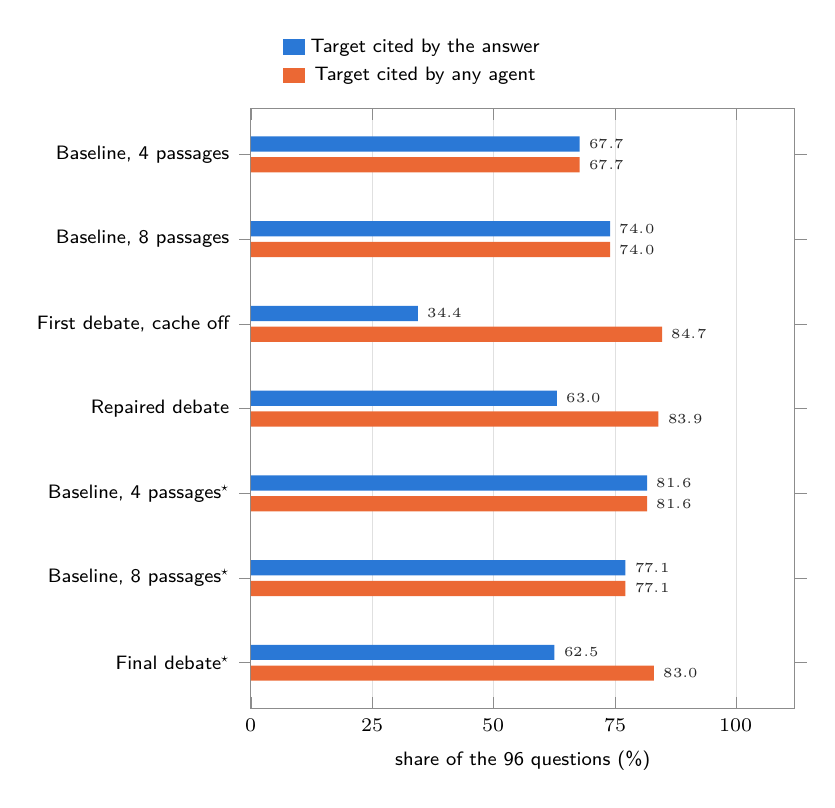
\begin{tikzpicture}
\begin{axis}[
    xbar, width=0.70\columnwidth, height=9.2cm,
    bar width=5.5pt, enlarge y limits=0.09,
    xmin=0, xmax=112, xtick={0,25,50,75,100},
    xlabel={share of the \ResTestCases\ questions (\%)},
    symbolic y coords={G,F,E,D,C,B,A},
    ytick={G,F,E,D,C,B,A},
    yticklabels={{Final debate$^{\star}$},{Baseline, 8 passages$^{\star}$},{Baseline, 4 passages$^{\star}$},{Repaired debate},{First debate, cache off},{Baseline, 8 passages},{Baseline, 4 passages}},
    y tick label style={font=\sffamily\scriptsize, align=right},
    x tick label style={font=\sffamily\scriptsize}, xlabel style={font=\sffamily\scriptsize},
    xmajorgrids, grid style={black!12}, axis line style={black!45}, tick style={black!45},
    nodes near coords, nodes near coords style={font=\sffamily\tiny, text=black!85, /pgf/number format/.cd, fixed, fixed zerofill, precision=1},
    legend style={font=\sffamily\scriptsize, draw=none, fill=none, at={(0.30,1.02)}, anchor=south, legend columns=1},
    legend image code/.code={\draw[#1, draw=none] (0cm,-0.09cm) rectangle (0.28cm,0.11cm);},
    reverse legend,
]
\addplot[fill=cPros, draw=none] coordinates {(\ResPaFinalTargetAny,G) (\ResPaBaseEightRTargetAny,F) (\ResPaBaseFourRTargetAny,E) (\ResPaFullTargetAny,D) (\ResPaOldTargetAny,C) (\ResPaBaseEightTargetAny,B) (\ResPaBaseFourTargetAny,A)};
\addlegendentry{Target cited by any agent}
\addplot[fill=cRetr, draw=none] coordinates {(\ResPaFinalTargetAnswer,G) (\ResPaBaseEightRTargetAnswer,F) (\ResPaBaseFourRTargetAnswer,E) (\ResPaFullTargetAnswer,D) (\ResPaOldTargetAnswer,C) (\ResPaBaseEightTargetAnswer,B) (\ResPaBaseFourTargetAnswer,A)};
\addlegendentry{Target cited by the answer}
\end{axis}
\end{tikzpicture}

\caption{Share of questions for which the target decision is cited by the final answer and by any agent, for the configurations on the earlier retrieval (upper four) and, marked $\star$, on the retrieval trained for retrieval (Section~\ref{sec:remaining}). For a baseline the two coincide. Every debate finds the target more often than its answer uses it.}\label{fig:pamain}
\end{figure}

\subsection{Ablation of the Repaired System}
Table~\ref{tab:paablation} and Fig.~\ref{fig:paablation} report the variants. In answers resting on the target, none of them differs significantly from the full system.

\emph{Defense (A1).} Without the defense, the share of answers resting on the target is the highest of all variants (\ResPaAOneTargetAnswer\% against \ResPaFullTargetAnswer\%; \cmp{FullAOne}{TargetAnswer}{\pp}, full system minus variant). The run also takes \ResPaAOneMinutes\ instead of \ResPaFullMinutes\ minutes, because the controller then ends a debate after \ResPaAOneRounds\ rounds on average. We could not measure any benefit of the defense, although none of our measures asks whether an unsupported claim was challenged.

\emph{Checker (A2).} Without the checker, the judge relies on its own citations and reports its own confidence (\ResPaATwoConf\ against \ResPaFullConf). With the checker, \ResPaFullNoAuthority\% of the answers rest on no existing authority, against \ResPaATwoNoAuthority\% without it (\cmp{FullATwo}{NoAuthority}{\pp}; \cmpword{FullATwo}{NoAuthority}), because the judge loses the citations whose holding the checker does not find shown. Of the \ResPaATwoCitationsMade\ citations made by the agents of this variant, \ResPaATwoNotFound\ name a non-existent case. The first debate, where a checker is active, produced \ResPaOldNotFound\ among \ResPaOldCitationsMade, so we cannot attribute these citations to the missing checker. In neither configuration did such a citation reach an answer.

\emph{Memory (A3).} Removing the memory changes no measure significantly. We expected this under the repaired cache rule, which cannot answer distinct questions. What is left of the memory in the full system is the risk index.

\emph{Later rounds (A4).} A debate limited to one round cites the target somewhere in \ResPaAFourTargetAny\% of cases, against \ResPaFullTargetAny\% for the full system (\ResCmpFullAFourTargetAnyP, \cmpword{FullAFour}{TargetAny}), yet its answers rest on the target just as often (\cmp{FullAFour}{TargetAnswer}{\pp}), in \ResPaAFourMinutes\ instead of \ResPaFullMinutes\ minutes. Whatever the later rounds find does not reach the answer. This is consistent with the overwriting of citations described in Section~\ref{sec:audit}.

\begin{table}[t]
\caption{Ablation of the repaired system (full system: \ResPaFullSeedsWord\ seeds; each variant: \ResPaAOneSeedsWord\ seed). An asterisk marks a significant paired difference from the full system.}\label{tab:paablation}
\centering
\footnotesize
\setlength{\tabcolsep}{2.4pt}
\begin{tabular}{@{}llrrrrrr@{}}
\toprule
 & Removed & \shortstack{Target\\in the\\answer\\(\%)} & \shortstack{Target\\by any\\agent\\(\%)} & \shortstack{No\\existing\\authority\\(\%)} & \shortstack{Confi-\\dence} & Rounds & \shortstack{Time\\(min)} \\
\midrule
Full & none & \ResPaFullTargetAnswer & \ResPaFullTargetAny & \ResPaFullNoAuthority & \ResPaFullConf & \ResPaFullRounds & \ResPaFullMinutes \\
A1 & defense & \ResPaAOneTargetAnswer\ResCmpFullAOneTargetAnswerMark & \ResPaAOneTargetAny\ResCmpFullAOneTargetAnyMark & \ResPaAOneNoAuthority\ResCmpFullAOneNoAuthorityMark & \ResPaAOneConf & \ResPaAOneRounds & \ResPaAOneMinutes \\
A2 & checker & \ResPaATwoTargetAnswer\ResCmpFullATwoTargetAnswerMark & \ResPaATwoTargetAny\ResCmpFullATwoTargetAnyMark & \ResPaATwoNoAuthority\ResCmpFullATwoNoAuthorityMark & \ResPaATwoConf & \ResPaATwoRounds & \ResPaATwoMinutes \\
A3 & memory & \ResPaAThreeTargetAnswer\ResCmpFullAThreeTargetAnswerMark & \ResPaAThreeTargetAny\ResCmpFullAThreeTargetAnyMark & \ResPaAThreeNoAuthority\ResCmpFullAThreeNoAuthorityMark & \ResPaAThreeConf & \ResPaAThreeRounds & \ResPaAThreeMinutes \\
A4 & later rounds & \ResPaAFourTargetAnswer\ResCmpFullAFourTargetAnswerMark & \ResPaAFourTargetAny\ResCmpFullAFourTargetAnyMark & \ResPaAFourNoAuthority\ResCmpFullAFourNoAuthorityMark & \ResPaAFourConf & \ResPaAFourRounds & \ResPaAFourMinutes \\
\bottomrule
\end{tabular}
\end{table}

\begin{figure*}[t]
\centering
% Fig. 6 - ablation of the repaired system, one panel per measure (full text width).
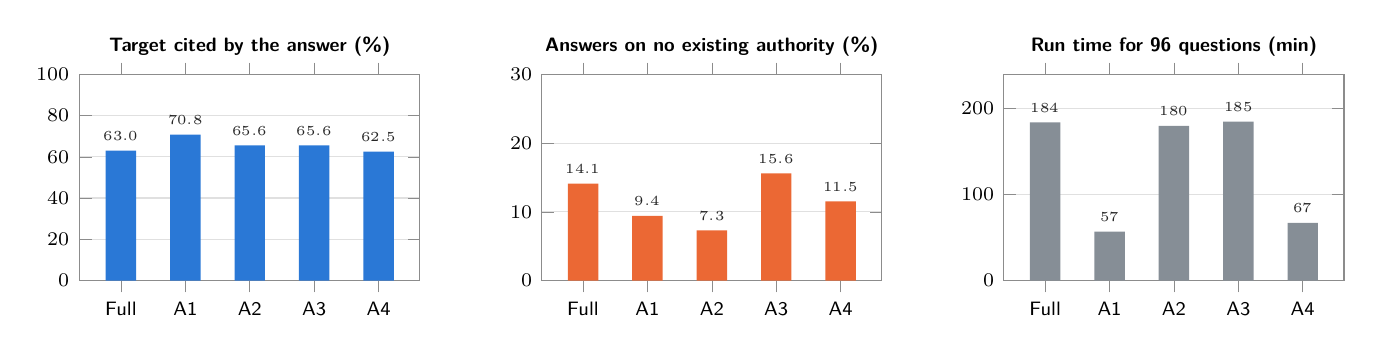
\begin{tikzpicture}
\begin{groupplot}[
    group style={group size=3 by 1, horizontal sep=1.55cm},
    ybar, width=5.9cm, height=4.2cm, /pgf/bar width=11pt,
    symbolic x coords={Full,A1,A2,A3,A4}, xtick=data, enlarge x limits=0.16,
    ymin=0,
    x tick label style={font=\sffamily\scriptsize}, y tick label style={font=\sffamily\scriptsize},
    title style={font=\sffamily\scriptsize\bfseries, yshift=-3pt},
    ymajorgrids, grid style={black!12}, axis line style={black!45}, tick style={black!45},
    nodes near coords, nodes near coords style={font=\sffamily\tiny, text=black!85},
]
\nextgroupplot[title={Target cited by the answer (\%)}, ymax=100,
    nodes near coords style={/pgf/number format/.cd, fixed, fixed zerofill, precision=1}]
\addplot[fill=cRetr, draw=none] coordinates {(Full,\ResPaFullTargetAnswer) (A1,\ResPaAOneTargetAnswer) (A2,\ResPaATwoTargetAnswer) (A3,\ResPaAThreeTargetAnswer) (A4,\ResPaAFourTargetAnswer)};
\nextgroupplot[title={Answers on no existing authority (\%)}, ymax=30,
    nodes near coords style={/pgf/number format/.cd, fixed, fixed zerofill, precision=1}]
\addplot[fill=cPros, draw=none] coordinates {(Full,\ResPaFullNoAuthority) (A1,\ResPaAOneNoAuthority) (A2,\ResPaATwoNoAuthority) (A3,\ResPaAThreeNoAuthority) (A4,\ResPaAFourNoAuthority)};
\nextgroupplot[title={Run time for \ResTestCases\ questions (min)}, ymax=240,
    nodes near coords style={/pgf/number format/.cd, fixed, precision=0}]
\addplot[fill=cNeutral, draw=none] coordinates {(Full,\ResPaFullMinutes) (A1,\ResPaAOneMinutes) (A2,\ResPaATwoMinutes) (A3,\ResPaAThreeMinutes) (A4,\ResPaAFourMinutes)};
\end{groupplot}
\end{tikzpicture}

\caption{Ablation of the repaired system. Each panel shows one measure for the full system and for the four variants that each remove one component (A1 defense, A2 citation checker, A3 memory, A4 rounds after the first).}\label{fig:paablation}
\end{figure*}

\subsection{Verdict Cache on a Workload With Repeats}\label{sec:cachetest}
The benchmark contains no repeated question, so it cannot show what a cache is for. We therefore built a workload with repeats. It consists of one pass of the repaired system, which stored \ResMemStored\ verdicts, followed by exact repeats of all questions, by variants that differ in case, punctuation and spacing, and by paraphrases written by the generator. Table~\ref{tab:memory} applies both cache rules to it. On the first pass the similarity rule returns a stored answer for \ResMemFirstPassOldWrong\ of \ResMemFirstPassQueries\ distinct questions, and every one of those answers belongs to another question. The same-question rule returns none on the first pass, serves all \ResMemRepeatNewCorrect\ stored verdicts on exact repeats and on format variants, and returns no wrong answer in any workload. It does not recognise paraphrases, which is the price of the rule. We could not measure how often a rejected citation recurs in a later session, because no citation failed the existence check in the first pass and so there was nothing to recur.

\begin{table}[t]
\caption{Verdict cache: hits of the two rules on four workloads. A hit is correct only if the stored answer was written for the same benchmark case.}\label{tab:memory}
\centering
\footnotesize
\setlength{\tabcolsep}{2.6pt}
\begin{tabular}{@{}lrrrrrrr@{}}
\toprule
 & & \multicolumn{3}{c}{Cosine $>0.92$} & \multicolumn{3}{c}{Same question} \\
\cmidrule(lr){3-5}\cmidrule(l){6-8}
Workload & Queries & Hits & Right & Wrong & Hits & Right & Wrong \\
\midrule
\ResRowsMemory
\bottomrule
\end{tabular}
\end{table}

% ════════════════════════════════════════════════════════════════════════════
\section{Remaining Repairs}\label{sec:remaining}
The repairs of Section~\ref{sec:repairs} left several defects of the audit in place. The traces saved by the repaired system allowed us to decide which of them mattered before making any further run.

\subsection{Evidence From the Traces}
In the first seed of the repaired debate, \ResLossLost\ of \ResLossCases\ debates cited the target decision and still returned an answer that does not rest on it. In \ResLossSupportedEarlierOnly\ of these, the target had been labelled \textsc{supported} in an earlier round but was no longer supported, or no longer cited, in the last round, which is the only round the judge reads. In \ResLossSupportedLastNotUsed\ it was supported in the last round and the judge did not list it, and in \ResLossNeverSupported\ it was never supported. Independently of the target, \ResLossAnswersEmptyAlthoughSupported\ answers rest on no citation even though the last round contained a supported one. We see two causes. First, the judge's instructions set score thresholds (0.75 for a citation it may rely on) that do not correspond to the checker's verdicts: \ResLossSupportedBelowJudgeThreshold\% of the \ResLossSupportedCitations\ citations labelled \textsc{supported} have a score below that value. Second, the controller never stops. The challenge strength that the defense reports for itself exceeded the threshold in \ResLossChallengeAboveThreshold\ of \ResLossRounds\ rounds, so every debate ran to the maximum and overwrote its own earlier results twice.

The risk index of the memory is a different matter. It handed a list to \ResLossAvoidDebates\ debates, but the lists contained only \ResLossAvoidNames\ distinct names in total, and the target of the question appeared on them in \ResLossAvoidOwnTarget\ cases. Removing the memory changed no measure (Section~\ref{sec:postaudit}), so we left it as it was. Retrieval, finally, limits every configuration from the outside: for \ResRetSystemMissEight\ of \ResRetQuestions\ questions the target opinion is not among the first-round passages.

\subsection{Ledger Protocol}
The second step of repairs changes how citations are handled across rounds.

\emph{Ledger.} For every decision cited in any round, a ledger keeps the best verdict it has received together with the passage that supported it. Entries are keyed by the report the citation resolves to, so two spellings of the same decision share one entry. A later, worse verdict never replaces an earlier, better one.

\emph{Judge.} The judge now reads the ledger of all rounds. Each verdict is given in words, each supported decision comes with its supporting passage, and the instructions refer to these verdicts instead of score thresholds. The program still decides what an answer rests on: a decision named by the judge counts only if the ledger holds it as \textsc{supported}. If the judge relied on a decision whose holding was not shown, we report that decision as uncertain instead of dropping it. A name written by the judge is matched to a ledger entry only when both parties agree. The earlier rule accepted any two shared words, which meant that one ``United States v.'' decision could stand in for another.

\emph{Controller.} A further round starts only if there is no supported citation yet, a gap remains, and the last round produced a new passage or a newly supported citation. The mean and minimum scores no longer force a round once a supported citation exists, and the self-reported challenge strength is no longer sufficient on its own:
\begin{equation}
\begin{aligned}
\text{continue} \iff\; & t < T_{\max} \;\land\; \lnot\,\mathrm{concede}_t \;\land\; |G_t| \geq 1 \\
& \land\; \lnot\,\mathrm{supported}_t \;\land\; \mathrm{new}_t .
\end{aligned}
\end{equation}

The audit had proposed letting the judge rely on any citation that exists and merely annotating missing support. We kept the stricter rule, so that an answer rests on supported citations only and the measure \emph{target cited by the answer} keeps the same meaning across all configurations.

\subsection{Retrieval Trained for Retrieval}
We replaced the dense retriever with an embedding model trained for retrieval (bge-base-en-v1.5~\cite{bge}), applied to the question alone, and we now compute BM25 over word tokens instead of whitespace tokens. As before, the first eight results of each ranking are fused. At most two passages of one decision are kept, and a list shortened by that limit is filled from deeper results under the same limit. We fixed the depth and the limit on design grounds and did not select them from the rows of Table~\ref{tab:retrieval}. The Legal-BERT index remains in place, because the support model was validated with it and the checker continues to use it. Table~\ref{tab:standard} gives the retrieval measures of both retrievers. Since a better retriever also helps a single agent, we ran the baselines again on the new retriever, and it is those baselines that the final system is compared with.

\subsection{Results of the Final System}
Table~\ref{tab:final} reports the final system, which carries both repairs, the two baselines on the same retriever, and two runs that carry one repair each. Table~\ref{tab:finaldiff} gives the paired differences, and Fig.~\ref{fig:pamain} shows all configurations side by side.

\emph{Retrieval.} The new retriever places a passage of the target opinion among its eight passages for \ResStdFinalHitEight\% of the questions (\ResStdFullHitEight\% before) and at the first rank for \ResStdFinalHitOne\% (\ResStdFullHitOne\% before). On its own, this lifts the four-passage baseline from \ResPaBaseFourTargetAnswer\% to \ResPaBaseFourRTargetAnswer\% of answers resting on the target (\cmp{BaseFourRBaseFour}{TargetAnswer}{\pp}).

\emph{The final debate.} The answers of the final system rest on the target in \ResPaFinalTargetAnswer\% of cases (\ResPaFinalTargetAnswerMin\% to \ResPaFinalTargetAnswerMax\% across the three seeds). This is no different from the repaired debate of Section~\ref{sec:postaudit} (\cmp{FinalFull}{TargetAnswer}{\pp}), and it is below both baselines on the same retriever: the four-passage baseline (\cmp{FinalBaseFourR}{TargetAnswer}{\pp}) and the eight-passage baseline (\cmp{FinalBaseEightR}{TargetAnswer}{\pp}). The agents cite the target somewhere in \ResPaFinalTargetAny\% of the debates, which is no longer more than a single agent cites (\cmp{FinalBaseFourR}{TargetAny}{\pp}). What the second step of repairs does deliver is a lower cost. A debate now ends after \ResPaFinalRounds\ rounds on average and takes \ResPaFinalSecondsPerCase\,s instead of \ResPaFullSecondsPerCase\,s, with an outcome that is statistically unchanged.

\emph{Attribution.} To see what each repair contributes, we ran each one alone. With the ledger protocol alone, on the earlier retriever, the answers rest on the target in \ResPaLedgerOnlyTargetAnswer\% of cases (\cmp{LedgerOnlyFull}{TargetAnswer}{\pp} against the repaired debate; \cmpword{LedgerOnlyFull}{TargetAnswer}). The target is cited somewhere less often (\ResPaLedgerOnlyTargetAny\%; \cmp{LedgerOnlyFull}{TargetAny}{\pp}), because two rounds of search are no longer run. With the new retriever alone, under the earlier protocol, the agents cite the target in \ResPaRetrievalOnlyTargetAny\% of the debates (\cmp{RetrievalOnlyFull}{TargetAny}{\pp}), while the answers rest on it in \ResPaRetrievalOnlyTargetAnswer\% (\cmp{RetrievalOnlyFull}{TargetAnswer}{\pp}; \cmpword{RetrievalOnlyFull}{TargetAnswer}). Better retrieval reaches the agents, but it does not reach the answer.

\emph{Where the loss occurs now.} Across the \ResFinalLossCases\ debates of the final system, an agent cites the target in \ResFinalLossCited\ and the answer rests on it in \ResFinalLossInAnswer. That leaves \ResFinalLossLost\ debates in which the target was cited and then lost. In \ResFinalLossLostSupported\ of them the ledger held the target as \textsc{supported}; the judge relied on a different supported decision in \ResFinalLossLostSupportedOtherCase\ of those and on none in \ResFinalLossLostSupportedNothing. In the remaining \ResFinalLossLostNotSupported, the passages read did not show the holding for which the agent had cited the target. On average a ledger holds \ResFinalLossSupportedPerDebate\ supported decisions per debate, and \ResFinalLossEmptyAlthoughSupported\ answers rest on nothing although one was available. The loss has therefore moved. It no longer comes from the bookkeeping, which the ledger repaired, but from the choice the judge makes among supported decisions and from the holdings that agents attach to the right case.

\begin{table}[t]
\caption{Second step of repairs, on the retrieval trained for retrieval unless stated: mean over the seeds of each configuration}\label{tab:final}
\centering
\footnotesize
\setlength{\tabcolsep}{2.3pt}
\begin{tabular}{@{}lrrrrr@{}}
\toprule
Measure & \shortstack{Base-\\line\\4 pass.} & \shortstack{Base-\\line\\8 pass.} & \shortstack{Ledger\\only$^{\ddagger}$} & \shortstack{Retrie-\\val\\only} & \shortstack{Final\\debate} \\
\midrule
Seeds & \ResPaBaseFourRSeeds & \ResPaBaseEightRSeeds & \ResPaLedgerOnlySeeds & \ResPaRetrievalOnlySeeds & \ResPaFinalSeeds \\
Target cited by the answer (\%) & \ResPaBaseFourRTargetAnswer & \ResPaBaseEightRTargetAnswer & \ResPaLedgerOnlyTargetAnswer & \ResPaRetrievalOnlyTargetAnswer & \ResPaFinalTargetAnswer \\
Target cited by any agent (\%) & \ResPaBaseFourRTargetAny & \ResPaBaseEightRTargetAny & \ResPaLedgerOnlyTargetAny & \ResPaRetrievalOnlyTargetAny & \ResPaFinalTargetAny \\
Citations the answer rests on & \ResPaBaseFourRCitesAnswer & \ResPaBaseEightRCitesAnswer & \ResPaLedgerOnlyCitesAnswer & \ResPaRetrievalOnlyCitesAnswer & \ResPaFinalCitesAnswer \\
Answers on no authority (\%) & \ResPaBaseFourRNoAuthority & \ResPaBaseEightRNoAuthority & \ResPaLedgerOnlyNoAuthority & \ResPaRetrievalOnlyNoAuthority & \ResPaFinalNoAuthority \\
Non-existent cases in answers & \ResPaBaseFourRNotFoundAnswer & \ResPaBaseEightRNotFoundAnswer & \ResPaLedgerOnlyNotFoundAnswer & \ResPaRetrievalOnlyNotFoundAnswer & \ResPaFinalNotFoundAnswer \\
Answer similarity & \ResPaBaseFourRSim & \ResPaBaseEightRSim & \ResPaLedgerOnlySim & \ResPaRetrievalOnlySim & \ResPaFinalSim \\
Mean confidence & \ResPaBaseFourRConf & \ResPaBaseEightRConf & \ResPaLedgerOnlyConf & \ResPaRetrievalOnlyConf & \ResPaFinalConf \\
Mean rounds & \ResPaBaseFourRRounds & \ResPaBaseEightRRounds & \ResPaLedgerOnlyRounds & \ResPaRetrievalOnlyRounds & \ResPaFinalRounds \\
Seconds per question & \ResPaBaseFourRSecondsPerCase & \ResPaBaseEightRSecondsPerCase & \ResPaLedgerOnlySecondsPerCase & \ResPaRetrievalOnlySecondsPerCase & \ResPaFinalSecondsPerCase \\
\bottomrule
\multicolumn{6}{@{}l}{$^{\ddagger}$ on the earlier retrieval.}
\end{tabular}
\end{table}

\begin{table}[t]
\caption{Paired differences of the final debate from the other configurations (percentage points for the first three measures of each block)}\label{tab:finaldiff}
\centering
\footnotesize
\setlength{\tabcolsep}{3.0pt}
\begin{tabular}{@{}lrll@{}}
\toprule
Measure & $\Delta$ & 95\% interval & Test \\
\midrule
\multicolumn{4}{@{}l}{\emph{Final debate minus baseline with 4 passages, same retrieval}} \\
\cmprow{Target cited by the answer}{FinalBaseFourR}{TargetAnswer}
\cmprow{Target cited by any agent}{FinalBaseFourR}{TargetAny}
\cmprow{Answers on no existing authority}{FinalBaseFourR}{NoAuthority}
\cmprow{Answer similarity}{FinalBaseFourR}{Sim}
\midrule
\multicolumn{4}{@{}l}{\emph{Final debate minus baseline with 8 passages, same retrieval}} \\
\cmprow{Target cited by the answer}{FinalBaseEightR}{TargetAnswer}
\cmprow{Target cited by any agent}{FinalBaseEightR}{TargetAny}
\cmprow{Answers on no existing authority}{FinalBaseEightR}{NoAuthority}
\cmprow{Answer similarity}{FinalBaseEightR}{Sim}
\midrule
\multicolumn{4}{@{}l}{\emph{Final debate minus repaired debate}} \\
\cmprow{Target cited by the answer}{FinalFull}{TargetAnswer}
\cmprow{Target cited by any agent}{FinalFull}{TargetAny}
\cmprow{Answers on no existing authority}{FinalFull}{NoAuthority}
\cmprow{Answer similarity}{FinalFull}{Sim}
\bottomrule
\multicolumn{4}{@{}l}{$^{\ast}$ $p < 0.05$ and the interval excludes zero.}
\end{tabular}
\end{table}

% ════════════════════════════════════════════════════════════════════════════
\section{Standard Measures and Comparison With Related Work}\label{sec:comparison}
We designed the measures used so far to state exactly what our system does. To set the results beside other work, we also scored every run with measures that other studies report, computed in the same way for the baseline and for the debate from the saved answers.

\subsection{Measures}
\emph{Retrieval.} Hit@$k$ is the share of questions for which a passage of the target opinion is among the first $k$ passages of the first retrieval; with one relevant opinion per question it equals Recall@$k$. MRR is the mean reciprocal rank of the first such passage among eight.

\emph{Fabricated citations.} Following the existence test of Dahl \emph{et al.}~\cite{dahl2024}, the share of citations, and of answers, that name a case which does not exist.

\emph{Citation recall and precision.} We apply the definitions of ALCE~\cite{alce} to case citations. Recall is the share of the sentences of the final answer that at least one cited opinion supports. Precision is the share of citations that support at least one sentence of the answer. Support is judged by the support model that passed the validation of Section~\ref{sec:validation}, at its validated threshold, on the three passages of the cited opinion closest to the sentence. Citations to real decisions outside the corpus cannot be checked, and we leave them out of precision.

\emph{Grounding outcome.} Following the classification of Magesh \emph{et al.}~\cite{magesh2025}, we call an answer \emph{grounded} if it cites at least one authority and every checkable citation exists and supports one of its sentences, \emph{misgrounded} if it cites a case that does not exist or that supports none of its sentences, and \emph{without authority} otherwise. The classification is automatic and says nothing about whether the answer is legally correct.

\emph{Answer overlap.} ROUGE-L, BERTScore (roberta-large) and token F1 of the final answer against the reference holding. \emph{Authority accuracy} is the share of answers that rest on the target decision.

\subsection{Results}
Table~\ref{tab:standard} reports the seven main configurations, and Fig.~\ref{fig:standard} shows the four measures of authority and grounding for the configurations on the new retriever. On the same retriever, the final debate trails the four-passage baseline in authority accuracy (\ResStdFinalAuthorityAccuracy\% against \ResStdBaseFourRAuthorityAccuracy\%), citation precision (\ResStdFinalCitationPrecision\% against \ResStdBaseFourRCitationPrecision\%), citation recall (\ResStdFinalCitationRecall\% against \ResStdBaseFourRCitationRecall\%), grounded answers (\ResStdFinalGrounded\% against \ResStdBaseFourRGrounded\%; \ResStdCmpFinalBaseFourRGroundedDiff\pp, \ResStdCmpFinalBaseFourRGroundedP), ROUGE-L (\ResStdFinalRougeL\ against \ResStdBaseFourRRougeL; \ResStdCmpFinalBaseFourRRougeLP) and BERTScore (\ResStdFinalBertScore\ against \ResStdBaseFourRBertScore; \ResStdCmpFinalBaseFourRBertScoreP). The lower citation precision is worth noting, because every citation a debate answer rests on had already been labelled \textsc{supported}. The explanation is that the checker verifies the holding an agent asserted, whereas the answer the judge writes afterwards is a different text.

Against the debate first evaluated, the final debate has a much higher authority accuracy (\ResStdCmpFinalOldAuthorityAccuracyDiff\pp, \ResStdCmpFinalOldAuthorityAccuracyP) and more grounded answers (\ResStdCmpFinalOldGroundedDiff\pp, \ResStdCmpFinalOldGroundedP). It also has more misgrounded answers (\ResStdCmpFinalOldMisgroundedDiff\pp), simply because answers that used to cite nothing now cite something. The one measure on which a debate is ahead of a single agent is existence. No answer of any debate cites a non-existent case, whereas \ResStdBaseEightRAnswersFabricated\% of the eight-passage baseline answers on the same retriever do (\ResStdBaseEightRFabricatedCount\ of \ResStdBaseEightRCitations\ citations). With so few events, however, the difference is \ResStdCmpFinalBaseEightRAnswersFabricatedWord\ (\ResStdCmpFinalBaseEightRAnswersFabricatedP).

\begin{table*}[t]
\caption{Standard measures, computed in the same way for every configuration (mean over seeds). Support is judged by the validated support model. Rates in per cent.}\label{tab:standard}
\centering
\footnotesize
\setlength{\tabcolsep}{5pt}
\begin{tabular}{@{}lrrrrrrr@{}}
\toprule
 & \multicolumn{4}{c}{Earlier retrieval (Legal-BERT + BM25)} & \multicolumn{3}{c}{Retrieval trained for retrieval} \\
\cmidrule(lr){2-5}\cmidrule(l){6-8}
Measure & \shortstack{Baseline\\4 passages} & \shortstack{Baseline\\8 passages} & \shortstack{First debate,\\cache off} & \shortstack{Repaired\\debate} & \shortstack{Baseline\\4 passages} & \shortstack{Baseline\\8 passages} & \shortstack{Final\\debate} \\
\midrule
\ResRowsStandard
\bottomrule
\end{tabular}
\end{table*}

\begin{figure}[t]
\centering
% Fig. 7 - standard measures of authority and grounding on the retrieval trained for retrieval (column width).
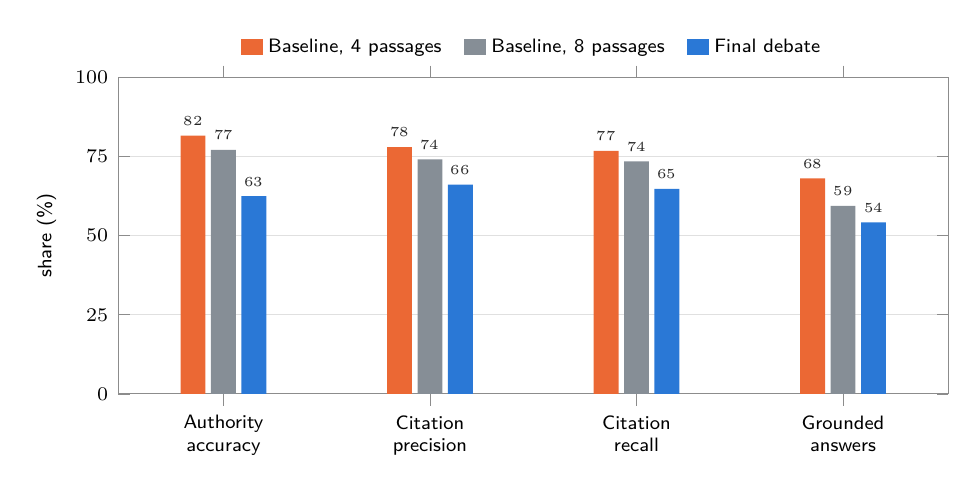
\begin{tikzpicture}
\begin{axis}[
    ybar, width=\columnwidth, height=5.6cm,
    /pgf/bar width=9pt, enlarge x limits=0.17,
    ymin=0, ymax=100, ytick={0,25,50,75,100},
    ylabel={share (\%)}, ylabel style={font=\sffamily\scriptsize},
    symbolic x coords={A,P,R,G},
    xtick={A,P,R,G},
    xticklabels={{Authority\\accuracy},{Citation\\precision},{Citation\\recall},{Grounded\\answers}},
    x tick label style={font=\sffamily\scriptsize, align=center}, y tick label style={font=\sffamily\scriptsize},
    ymajorgrids, grid style={black!12}, axis line style={black!45}, tick style={black!45},
    nodes near coords, nodes near coords style={font=\sffamily\tiny, text=black!85, /pgf/number format/.cd, fixed, precision=0},
    legend style={font=\sffamily\scriptsize, draw=none, fill=none, at={(0.5,1.03)}, anchor=south, legend columns=3, /tikz/every even column/.append style={column sep=6pt}},
    legend image code/.code={\draw[#1, draw=none] (0cm,-0.09cm) rectangle (0.28cm,0.11cm);},
]
\addplot[fill=cPros, draw=none] coordinates {(A,\ResStdBaseFourRAuthorityAccuracy) (P,\ResStdBaseFourRCitationPrecision) (R,\ResStdBaseFourRCitationRecall) (G,\ResStdBaseFourRGrounded)};
\addlegendentry{Baseline, 4 passages}
\addplot[fill=cNeutral, draw=none] coordinates {(A,\ResStdBaseEightRAuthorityAccuracy) (P,\ResStdBaseEightRCitationPrecision) (R,\ResStdBaseEightRCitationRecall) (G,\ResStdBaseEightRGrounded)};
\addlegendentry{Baseline, 8 passages}
\addplot[fill=cRetr, draw=none] coordinates {(A,\ResStdFinalAuthorityAccuracy) (P,\ResStdFinalCitationPrecision) (R,\ResStdFinalCitationRecall) (G,\ResStdFinalGrounded)};
\addlegendentry{Final debate}
\end{axis}
\end{tikzpicture}

\caption{Standard measures of authority and grounding on the retrieval trained for retrieval. The single agent is ahead of the final debate on all four; exact values are in Table~\ref{tab:standard}.}\label{fig:standard}
\end{figure}

\subsection{Comparison With Results Reported in Related Work}
Table~\ref{tab:reported} places our results next to the figures reported by the most closely related studies. The entries are not directly comparable. Each study uses its own task, data, model and definition of error, and we quote the values as the authors report them. Four observations can still be made.

\emph{Hallucination rates.} General-purpose models hallucinate in 58\% to 88\% of verifiable questions about federal cases~\cite{dahl2024}, and commercial retrieval-augmented research tools do so in 17\% to 33\% of queries~\cite{magesh2025}. In our runs, fabricated case citations are rare in every configuration (at most \ResStdBaseEightRCitationsFabricated\% of citations) and absent from the answers of the debates. We attribute this mainly to retrieval grounding on a closed corpus, and only to a small extent to the debate. The measure closer to that of Magesh \emph{et al.}, who count misgrounded statements, is our share of misgrounded answers: \ResStdFinalMisgrounded\% for the final debate and \ResStdBaseFourRMisgrounded\% for the four-passage baseline. Both are near or above the upper end of the range those authors report for commercial tools, although our definition is automatic and counts every citation that supports no sentence of the answer.

\emph{Citation quality.} Gao \emph{et al.} report that even the best systems they evaluate lack complete citation support for half of their answers on one of their datasets~\cite{alce}. Under our adapted definitions, a cited opinion supports \ResStdBaseFourRCitationRecall\% of the answer sentences of the baseline and \ResStdFinalCitationRecall\% of those of the final debate.

\emph{Verification.} HalluGraph reports an AUC of 0.979 on structured control documents and 0.89 on generative legal tasks for detecting unfaithful output~\cite{hallugraph}. Our first checker reached \ResStressAUC. The validated support model reaches \ResGateTestAUC\ on held-out citations, but on a test whose incorrect holdings come from unrelated cases, and it still accepts \ResProbeNearMissPct\% of near-miss holdings.

\emph{Gains from debate.} PROClaim reports a gain of 10.0 percentage points in accuracy over standard multi-agent debate on claim verification~\cite{proclaim}, AgentCourt a 12.1\% improvement of its evolved lawyer agents~\cite{agentcourt}, and ChatLaw and LRAS report gains over single-model baselines~\cite{chatlaw,lras}. We obtained no such gain. On the same retriever, the authority accuracy of the final debate differs from that of its single-agent baseline by \ResCmpFinalBaseFourRTargetAnswerDiff\pp.

\begin{table*}[t]
\caption{Results reported by related work and the corresponding results of this work. Values are quoted as reported; tasks, data and error definitions differ, so rows are not directly comparable.}\label{tab:reported}
\centering
\footnotesize
\setlength{\tabcolsep}{4pt}
\begin{tabular}{@{}p{0.19\textwidth}p{0.31\textwidth}p{0.25\textwidth}p{0.18\textwidth}@{}}
\toprule
Work & Task and data & Measure & Result \\
\midrule
\multicolumn{4}{@{}l}{\emph{Hallucination in legal question answering}} \\
Dahl \emph{et al.}~\cite{dahl2024} & General-purpose LLMs; verifiable questions about random U.S. federal court cases & Hallucination rate & 58\% (GPT-4) to 88\% (Llama~2) \\
Magesh \emph{et al.}~\cite{magesh2025} & Commercial legal research tools built on RAG (Lexis+ AI, Westlaw AI-Assisted Research, Ask Practical Law AI) & Hallucination rate (false or misgrounded) & 17\% to 33\% \\
\textbf{This work}, single-agent RAG, 4 passages & \ResTestCases\ questions on U.S. Supreme Court decisions; Mistral-7B, retrieval trained for retrieval & Answers citing a non-existent case; answers misgrounded & \ResStdBaseFourRAnswersFabricated\%; \ResStdBaseFourRMisgrounded\% \\
\textbf{This work}, single-agent RAG, 8 passages & Same & Same & \ResStdBaseEightRAnswersFabricated\%; \ResStdBaseEightRMisgrounded\% \\
\textbf{This work}, final \sys & Same questions; debate with validated checker and ledger & Same & \ResStdFinalAnswersFabricated\%; \ResStdFinalMisgrounded\% \\
\midrule
\multicolumn{4}{@{}l}{\emph{Citation quality}} \\
ALCE, Gao \emph{et al.}~\cite{alce} & Question answering with citations; ELI5 & Answers lacking complete citation support, best systems & 50\% \\
\textbf{This work}, single-agent RAG, 4 passages & As above & Citation recall; citation precision (ALCE definitions, validated support model) & \ResStdBaseFourRCitationRecall\%; \ResStdBaseFourRCitationPrecision\% \\
\textbf{This work}, final \sys & As above & Same & \ResStdFinalCitationRecall\%; \ResStdFinalCitationPrecision\% \\
\midrule
\multicolumn{4}{@{}l}{\emph{Verification and hallucination detection}} \\
HalluGraph~\cite{hallugraph} & Detection of unfaithful output in legal RAG by knowledge-graph alignment & Area under the ROC curve & 0.979 (structured control documents); 0.89 (generative legal tasks) \\
\textbf{This work}, first checker & \ResStressTotal\ labelled citations (correct, swapped holding, false holding, invented, outside corpus) & Invented citations rejected; correct citations accepted; area, correct against swapped holdings & 100\%; \ResStressCorrectAcceptedPct\%; \ResStressAUC \\
\textbf{This work}, validated support model & Held-out half of the correct, swapped and false holdings; near-miss probe & Area, correct against incorrect holdings; correct accepted; near-miss holdings accepted & \ResGateTestAUC; \ResProbeCorrectPct\%; \ResProbeNearMissPct\% \\
\midrule
\multicolumn{4}{@{}l}{\emph{Multi-agent and agentic systems}} \\
PROClaim~\cite{proclaim} & Courtroom-style debate with progressive retrieval; claim verification on Check-COVID & Accuracy; gain over standard multi-agent debate & 81.7\%; +10.0\pp \\
AgentCourt~\cite{agentcourt} & Adversarially evolved lawyer agents; CourtBench, after 1{,}000 simulated civil cases & Improvement of evolved over original agents & +12.1\% \\
ChatLaw~\cite{chatlaw} & Cooperative multi-agent assistant for Chinese law; LawBench and the Unified Qualification Exam for Legal Professionals & Gain over GPT-4 & +7.73\% accuracy; +11 points \\
LRAS~\cite{lras} & Legal reasoning with agentic search & Gain over state-of-the-art baselines & 8.2\% to 32\% \\
\textbf{This work}, final \sys\ against single-agent RAG on the same retrieval & \ResTestCases\ questions on U.S. Supreme Court decisions & Authority accuracy; difference from the 4-passage and the 8-passage baseline & \ResStdFinalAuthorityAccuracy\%; \ResCmpFinalBaseFourRTargetAnswerDiff\pp\ and \ResCmpFinalBaseEightRTargetAnswerDiff\pp \\
\bottomrule
\end{tabular}
\end{table*}

% ════════════════════════════════════════════════════════════════════════════
\section{Discussion and Limitations}

\emph{What the audit changes.} In effect, our first evaluation measured its own cache. A third of its debates never took place, and the two measures on which the baseline was recorded as better do not measure what their names suggest. The stress test of the verifier is the one part of that evaluation that stands unchanged, and it was the part that led us to the next defect.

\emph{The corrected evaluation was wrong as well.} The runs we made after the audit reproduced an error from the first evaluation that the audit had missed: the baseline parser discarded citations written as strings. Until we corrected it, the eight-passage baseline appeared to cite the target in \ResParseBaseEightTargetAsSaved\% of its answers when it actually did so in \ResPaBaseEightTargetAnswer\%, and the debate appeared to be level with the single agent when it was in fact behind. This error favoured the method under study, just as the cache had worked against it. We found it only because an implausible number made us go back to the raw outputs, and we could correct it without a new run only because the first repair saves those outputs. We take two practical lessons from this. A run that saves only parsed fields and aggregate scores cannot be audited. And an audit has to cover the baseline as carefully as the system under study.

\emph{What the repairs achieve.} The repairs roughly double the share of debate answers that rest on the target decision, from \ResPaOldTargetAnswer\% to \ResPaFinalTargetAnswer\%. They reduce answers without authority from \ResPaOldNoAuthority\% to \ResPaFinalNoAuthority\% and shorten a debate from \ResPaOldSecondsPerCase\ to \ResPaFinalSecondsPerCase\ seconds. The support model chosen by validation separates correct from incorrect holdings, which the default model could not do, and no debate answer rests on a non-existent case.

\emph{What the debate does not achieve.} On no measure of the final answer other than existence is the debate ahead of a single agent with the same retriever, and on most it is significantly behind. More of the single agent's answers rest on the target, more of its sentences are supported by what it cites, its answers overlap more with the reference holdings, and it answers about \ResPaFinalTimeRatio\ times faster. This holds at both context sizes. None of the ablation variants differs significantly from the full system, so we cannot show that any single component contributes. The agents of a debate still cite the target in \ResPaFinalTargetAny\% of cases, but a single agent with four passages does so in \ResPaBaseFourRTargetAny\%, and its answer keeps what it cites.

\emph{Why.} We can offer three observations on the cause, none of which settles it. First, the answer of a debate rests on \ResPaFinalCitesAnswer\ decisions on average, which the judge selects from a ledger holding \ResFinalLossSupportedPerDebate\ supported ones, while a single agent names every decision it used (\ResPaBaseFourRCitesAnswer\ per answer). The target is lost in that selection in \ResFinalLossLostSupported\ of \ResFinalLossCases\ debates. Second, the checker verifies the holding that an agent attached to a citation, not the answer that is finally given, so verified citations do not add up to a verified answer. This is visible in the citation precision of debate answers, which is lower than that of the baseline. Third, the generator is a 7-billion-parameter model that has to play four roles in sequence. We did not test whether a stronger generator would make better use of the debate.

\emph{Limitations.} Our benchmark contains \ResTestCases\ questions on United States Supreme Court decisions with one target decision each. The conclusions do not extend to other courts, jurisdictions or question types, and we do not measure the relevance of citations other than the target. A measure that asks whether an answer names the target favours answers that name several decisions, which is why we also report citation precision. The final system, the first debate and all baselines have three seeds, the repaired debate has two, and its ablation variants and the two attribution runs have one. Between seeds, the share of answers resting on the target has a standard deviation of \ResPaFinalTargetAnswerSD\ percentage points for the final debate, \ResPaOldTargetAnswerSD\ for the first debate and \ResPaBaseFourRTargetAnswerSD\ for the four-passage baseline. We evaluated one generator at one temperature. The support model was validated on citations built from the reference holdings of the same benchmark, with incorrect holdings taken from unrelated cases, and it accepts \ResProbeNearMissPct\% of near-miss holdings. The same model judges citation support in the standard measures, for the baseline and the debate alike. None of our measures scores the legal correctness of an answer. The baseline of the first evaluation cannot be corrected. Finally, volumes 573 to 593 contain opinions extracted from PDF without order entries, and the most recent of them is partial.

\emph{Implications.} One design decision held up throughout: separating the question of whether a citation exists from the question of whether it supports the claim. Both versions of the checker answered the existence question reliably, and the support question became answerable once we chose the model by validation. The debate built around the checker did not hold up on this benchmark. The natural next system is a single agent followed by the checker, which would keep the answer of the stronger configuration and remove the citations that do not exist or do not support it. The runs reported here already contain what is needed to estimate it. Whether adversarial debate helps with a stronger generator, with questions that have no single landmark answer, or with a judge that reads the checked answer instead of only checked citations, remains an open question.

% ════════════════════════════════════════════════════════════════════════════
\section{Conclusion}
We presented \sys, a multi-agent debate framework for legal question answering in which citation verification, debate control and memory operate inside the debate loop, together with a resumable pipeline that builds a \ResCorpusVolumes-volume corpus of the United States Reports. We also audited our own evaluation of that framework twice. The first evaluation was distorted by a similarity-keyed verdict cache that replaced \ResAudCacheBench\ of \ResTestCases\ debates with answers to other questions, by measures that did not measure what they named, and by an entailment model that had not been validated. The second was distorted by a baseline parser that discarded citations written as strings. After six repairs to the system and corrections to both evaluations, the debate is a much better debate than the one we started with. \ResPaFinalTargetAnswer\% of its answers rest on the target decision instead of \ResPaOldTargetAnswer\%, in \ResPaFinalSecondsPerCase\ seconds instead of \ResPaOldSecondsPerCase, with a support model that passed a held-out validation at an AUC of \ResGateTestAUC\ and with no non-existent case in any answer. It is nevertheless not a better system than a single agent. On the same retriever, the single-agent baseline rests on the target in \ResPaBaseFourRTargetAnswer\% of its answers, scores higher on citation recall, citation precision, grounded answers, ROUGE-L and BERTScore, and needs \ResPaBaseFourRSecondsPerCase\ seconds. For this benchmark and a 7-billion-parameter generator, the only contribution of adversarial debate with in-loop verification that we could measure is the exclusion of non-existent citations. In future work we plan to apply the validated checker to the single agent's answer, to test the debate with a stronger generator and on questions without a single landmark answer, and to extend the benchmark beyond one jurisdiction.

\balance
\bibliographystyle{IEEEtran}
\begin{thebibliography}{00}
\bibitem{dahl2024} M.~Dahl, V.~Magesh, M.~Suzgun, and D.~E.~Ho, ``Large legal fictions: Profiling legal hallucinations in large language models,'' \emph{J. Legal Anal.}, vol.~16, no.~1, pp.~64--93, 2024.
\bibitem{magesh2025} V.~Magesh, F.~Surani, M.~Dahl, M.~Suzgun, C.~D.~Manning, and D.~E.~Ho, ``Hallucination-free? Assessing the reliability of leading AI legal research tools,'' \emph{J. Empirical Legal Stud.}, vol.~22, pp.~216--242, 2025.
\bibitem{mata2023} \emph{Mata v.\ Avianca, Inc.}, 678 F.~Supp.~3d 443 (S.D.N.Y. 2023).
\bibitem{sciwhitepaper2025} Centre for Research and Planning, Supreme Court of India, ``White paper on artificial intelligence and judiciary,'' New Delhi, India, Nov. 2025.
\bibitem{disclawllm} S.~Yue \emph{et al.}, ``DISC-LawLLM: Fine-tuning large language models for intelligent legal services,'' arXiv:2309.11325, 2023.
\bibitem{lawgpt} Z.~Zhou \emph{et al.}, ``LawGPT: A Chinese legal knowledge-enhanced large language model,'' arXiv:2406.04614, 2024.
\bibitem{lawformer} C.~Xiao, X.~Hu, Z.~Liu, C.~Tu, and M.~Sun, ``Lawformer: A pre-trained language model for Chinese legal long documents,'' \emph{AI Open}, vol.~2, pp.~79--84, 2021.
\bibitem{legalbench} N.~Guha \emph{et al.}, ``LegalBench: A collaboratively built benchmark for measuring legal reasoning in large language models,'' in \emph{Proc. Adv. Neural Inf. Process. Syst. (NeurIPS), Datasets and Benchmarks Track}, 2023.
\bibitem{lawbench} Z.~Fei \emph{et al.}, ``LawBench: Benchmarking legal knowledge of large language models,'' in \emph{Proc. Conf. Empirical Methods Natural Lang. Process. (EMNLP)}, 2024.
\bibitem{lexglue} I.~Chalkidis \emph{et al.}, ``LexGLUE: A benchmark dataset for legal language understanding in English,'' in \emph{Proc. Annu. Meeting Assoc. Comput. Linguistics (ACL)}, 2022, pp.~4310--4330.
\bibitem{legalagentbench} H.~Li \emph{et al.}, ``LegalAgentBench: Evaluating LLM agents in legal domain,'' arXiv:2412.17259, 2024.
\bibitem{lewis2020} P.~Lewis \emph{et al.}, ``Retrieval-augmented generation for knowledge-intensive NLP tasks,'' in \emph{Proc. Adv. Neural Inf. Process. Syst. (NeurIPS)}, 2020.
\bibitem{crag} S.-Q.~Yan, J.-C.~Gu, Y.~Zhu, and Z.-H.~Ling, ``Corrective retrieval augmented generation,'' arXiv:2401.15884, 2024.
\bibitem{hyparag} R.~Kalra \emph{et al.}, ``HyPA-RAG: A hybrid parameter adaptive retrieval-augmented generation system for AI legal and policy applications,'' arXiv:2409.09046, 2024.
\bibitem{lras} Y.~Zhou \emph{et al.}, ``LRAS: Advanced legal reasoning with agentic search,'' arXiv:2601.07296, 2026.
\bibitem{bm25} S.~Robertson and H.~Zaragoza, ``The probabilistic relevance framework: BM25 and beyond,'' \emph{Found. Trends Inf. Retr.}, vol.~3, no.~4, pp.~333--389, 2009.
\bibitem{legalbert} I.~Chalkidis, M.~Fergadiotis, P.~Malakasiotis, N.~Aletras, and I.~Androutsopoulos, ``LEGAL-BERT: The muppets straight out of law school,'' in \emph{Findings Assoc. Comput. Linguistics: EMNLP}, 2020, pp.~2898--2904.
\bibitem{rrf} G.~V.~Cormack, C.~L.~A.~Clarke, and S.~B\"uttcher, ``Reciprocal rank fusion outperforms Condorcet and individual rank learning methods,'' in \emph{Proc. Int. ACM SIGIR Conf. Res. Develop. Inf. Retr.}, 2009, pp.~758--759.
\bibitem{sectionhybrid} R.~Arulanandam and N.~de~Silva, ``Section-weighted hybrid approach for legal case retrieval,'' arXiv:2606.03138, 2026.
\bibitem{leakgraphrag} J.~Liu and J.~Tang, ``LeAK-GraphRAG: A legal academic knowledge GraphRAG framework with hybrid retrieval for mitigating hallucinations,'' in \emph{Legal Knowledge and Information Systems}, ser. Frontiers in Artificial Intelligence and Applications. IOS Press, 2025, doi: 10.3233/FAIA251624.
\bibitem{selfcheckgpt} P.~Manakul, A.~Liusie, and M.~J.~F.~Gales, ``SelfCheckGPT: Zero-resource black-box hallucination detection for generative large language models,'' in \emph{Proc. Conf. Empirical Methods Natural Lang. Process. (EMNLP)}, 2023, pp.~9004--9017.
\bibitem{cove} S.~Dhuliawala \emph{et al.}, ``Chain-of-verification reduces hallucination in large language models,'' in \emph{Findings Assoc. Comput. Linguistics: ACL}, 2024, pp.~3563--3578.
\bibitem{selfrag} A.~Asai, Z.~Wu, Y.~Wang, A.~Sil, and H.~Hajishirzi, ``Self-RAG: Learning to retrieve, generate, and critique through self-reflection,'' in \emph{Proc. Int. Conf. Learn. Represent. (ICLR)}, 2024.
\bibitem{hallugraph} V.~No\"el, E.~Y.~Seidou, C.~K.~Capo-Chichi, and G.~Amari, ``HalluGraph: Auditable hallucination detection for legal RAG systems via knowledge graph alignment,'' arXiv:2512.01659, 2025.
\bibitem{falkorirac} J.~Bose, ``Falkor-IRAC: Graph-constrained generation for verified legal reasoning in Indian judicial AI,'' arXiv:2605.14665, 2026.
\bibitem{du2024} Y.~Du, S.~Li, A.~Torralba, J.~B.~Tenenbaum, and I.~Mordatch, ``Improving factuality and reasoning in language models through multiagent debate,'' in \emph{Proc. Int. Conf. Mach. Learn. (ICML)}, 2024.
\bibitem{liang2024} T.~Liang \emph{et al.}, ``Encouraging divergent thinking in large language models through multi-agent debate,'' in \emph{Proc. Conf. Empirical Methods Natural Lang. Process. (EMNLP)}, 2024.
\bibitem{smit2024} A.~Smit, N.~Grinsztajn, P.~Duckworth, T.~D.~Barrett, and A.~Pretorius, ``Should we be going MAD? A look at multi-agent debate strategies for LLMs,'' in \emph{Proc. Int. Conf. Mach. Learn. (ICML)}, 2024.
\bibitem{metagpt} S.~Hong \emph{et al.}, ``MetaGPT: Meta programming for a multi-agent collaborative framework,'' in \emph{Proc. Int. Conf. Learn. Represent. (ICLR)}, 2024.
\bibitem{autogen} Q.~Wu \emph{et al.}, ``AutoGen: Enabling next-gen LLM applications via multi-agent conversation,'' arXiv:2308.08155, 2023.
\bibitem{chatlaw} J.~Cui \emph{et al.}, ``ChatLaw: A multi-agent collaborative legal assistant with knowledge graph enhanced mixture-of-experts large language model,'' arXiv:2306.16092, 2023.
\bibitem{agentcourt} G.~Chen \emph{et al.}, ``AgentCourt: Simulating court with adversarial evolvable lawyer agents,'' arXiv:2408.08089, 2024.
\bibitem{proclaim} M.~N.~Chowdhury, N.~J.~Beg, U.~H.~Khan, S.~R.~Raiyan, M.~K.~Hasan, and H.~Mahmud, ``Courtroom-style multi-agent debate with progressive RAG and role-switching for controversial claim verification,'' arXiv:2603.28488, 2026.
\bibitem{cap} Harvard Law School Library Innovation Lab, ``Caselaw Access Project.'' [Online]. Available: https://case.law
\bibitem{usreports} Supreme Court of the United States, ``United States Reports: Bound volumes and preliminary prints.'' [Online]. Available: https://www.supremecourt.gov/opinions/USReports.aspx
\bibitem{chroma} Chroma, ``Chroma: The open-source embedding database.'' [Online]. Available: https://github.com/chroma-core/chroma
\bibitem{mistral7b} A.~Q.~Jiang \emph{et al.}, ``Mistral 7B,'' arXiv:2310.06825, 2023.
\bibitem{debertav3} P.~He, J.~Gao, and W.~Chen, ``DeBERTaV3: Improving DeBERTa using ELECTRA-style pre-training with gradient-disentangled embedding sharing,'' in \emph{Proc. Int. Conf. Learn. Represent. (ICLR)}, 2023.
\bibitem{langgraph} LangChain, Inc., ``LangGraph.'' [Online]. Available: https://github.com/langchain-ai/langgraph
\bibitem{alce} T.~Gao, H.~Yen, J.~Yu, and D.~Chen, ``Enabling large language models to generate text with citations,'' in \emph{Proc. Conf. Empirical Methods Natural Lang. Process. (EMNLP)}, 2023.
\bibitem{sbert} N.~Reimers and I.~Gurevych, ``Sentence-BERT: Sentence embeddings using Siamese BERT-networks,'' in \emph{Proc. Conf. Empirical Methods Natural Lang. Process. (EMNLP)}, 2019, pp.~3982--3992.
\bibitem{mpnet} K.~Song, X.~Tan, T.~Qin, J.~Lu, and T.-Y.~Liu, ``MPNet: Masked and permuted pre-training for language understanding,'' in \emph{Proc. Adv. Neural Inf. Process. Syst. (NeurIPS)}, 2020.
\bibitem{tasksource} D.~Sileo, ``tasksource: A dataset harmonization framework for streamlined NLP multi-task learning and evaluation,'' arXiv:2301.05948, 2023.
\bibitem{bge} S.~Xiao, Z.~Liu, P.~Zhang, N.~Muennighoff, D.~Lian, and J.-Y.~Nie, ``C-Pack: Packed resources for general Chinese embeddings,'' arXiv:2309.07597, 2023.
\end{thebibliography}

\end{document}
